\documentclass[twoside]{book}

% Packages required by doxygen
\usepackage{fixltx2e}
\usepackage{calc}
\usepackage{doxygen}
\usepackage[export]{adjustbox} % also loads graphicx
\usepackage{graphicx}
\usepackage[utf8]{inputenc}
\usepackage{makeidx}
\usepackage{multicol}
\usepackage{multirow}
\PassOptionsToPackage{warn}{textcomp}
\usepackage{textcomp}
\usepackage[nointegrals]{wasysym}
\usepackage[table]{xcolor}

% Font selection
\usepackage[T1]{fontenc}
\usepackage[scaled=.90]{helvet}
\usepackage{courier}
\usepackage{amssymb}
\usepackage{sectsty}
\renewcommand{\familydefault}{\sfdefault}
\allsectionsfont{%
  \fontseries{bc}\selectfont%
  \color{darkgray}%
}
\renewcommand{\DoxyLabelFont}{%
  \fontseries{bc}\selectfont%
  \color{darkgray}%
}
\newcommand{\+}{\discretionary{\mbox{\scriptsize$\hookleftarrow$}}{}{}}

% Page & text layout
\usepackage{geometry}
\geometry{%
  a4paper,%
  top=2.5cm,%
  bottom=2.5cm,%
  left=2.5cm,%
  right=2.5cm%
}
\tolerance=750
\hfuzz=15pt
\hbadness=750
\setlength{\emergencystretch}{15pt}
\setlength{\parindent}{0cm}
\setlength{\parskip}{3ex plus 2ex minus 2ex}
\makeatletter
\renewcommand{\paragraph}{%
  \@startsection{paragraph}{4}{0ex}{-1.0ex}{1.0ex}{%
    \normalfont\normalsize\bfseries\SS@parafont%
  }%
}
\renewcommand{\subparagraph}{%
  \@startsection{subparagraph}{5}{0ex}{-1.0ex}{1.0ex}{%
    \normalfont\normalsize\bfseries\SS@subparafont%
  }%
}
\makeatother

% Headers & footers
\usepackage{fancyhdr}
\pagestyle{fancyplain}
\fancyhead[LE]{\fancyplain{}{\bfseries\thepage}}
\fancyhead[CE]{\fancyplain{}{}}
\fancyhead[RE]{\fancyplain{}{\bfseries\leftmark}}
\fancyhead[LO]{\fancyplain{}{\bfseries\rightmark}}
\fancyhead[CO]{\fancyplain{}{}}
\fancyhead[RO]{\fancyplain{}{\bfseries\thepage}}
\fancyfoot[LE]{\fancyplain{}{}}
\fancyfoot[CE]{\fancyplain{}{}}
\fancyfoot[RE]{\fancyplain{}{\bfseries\scriptsize Generated by Doxygen }}
\fancyfoot[LO]{\fancyplain{}{\bfseries\scriptsize Generated by Doxygen }}
\fancyfoot[CO]{\fancyplain{}{}}
\fancyfoot[RO]{\fancyplain{}{}}
\renewcommand{\footrulewidth}{0.4pt}
\renewcommand{\chaptermark}[1]{%
  \markboth{#1}{}%
}
\renewcommand{\sectionmark}[1]{%
  \markright{\thesection\ #1}%
}

% Indices & bibliography
\usepackage{natbib}
\usepackage[titles]{tocloft}
\setcounter{tocdepth}{3}
\setcounter{secnumdepth}{5}
\makeindex

% Hyperlinks (required, but should be loaded last)
\usepackage{ifpdf}
\ifpdf
  \usepackage[pdftex,pagebackref=true]{hyperref}
\else
  \usepackage[ps2pdf,pagebackref=true]{hyperref}
\fi
\hypersetup{%
  colorlinks=true,%
  linkcolor=blue,%
  citecolor=blue,%
  unicode%
}

% Custom commands
\newcommand{\clearemptydoublepage}{%
  \newpage{\pagestyle{empty}\cleardoublepage}%
}

\usepackage{caption}
\captionsetup{labelsep=space,justification=centering,font={bf},singlelinecheck=off,skip=4pt,position=top}

%===== C O N T E N T S =====

\begin{document}

% Titlepage & ToC
\hypersetup{pageanchor=false,
             bookmarksnumbered=true,
             pdfencoding=unicode
            }
\pagenumbering{alph}
\begin{titlepage}
\vspace*{7cm}
\begin{center}%
{\Large Wood\+Box Framework }\\
\vspace*{1cm}
{\large Generated by Doxygen 1.8.14}\\
\end{center}
\end{titlepage}
\clearemptydoublepage
\pagenumbering{roman}
\tableofcontents
\clearemptydoublepage
\pagenumbering{arabic}
\hypersetup{pageanchor=true}

%--- Begin generated contents ---
\chapter{Wood\+Box Development Kit}
\label{index}\hypertarget{index}{}This repository holds the source code of the Wood\+Box Development Kit (Framework + examples + P\+C\+Bs and schematics).

\subsection*{What is Wood\+Box?}

Wood\+Box is a set of smart devices enabling to monitor a house\textquotesingle{}s environment and the possible effects on human health. A smartphone application communicating with sensing devices put into the house, enable the user to get advices, tips and solutions to potential problems, and to communicate with other members of Wood\+Box community, to be able to live better at home.

\subsection*{Installation and requirements to use this kit\+:}

This development kit requires some external libraries to be present on your environment. If you use Arduino, just download these into your \char`\"{}libraries\char`\"{} folder into your \char`\"{}\+Arduino\char`\"{} directory.

In the same way, to use this development kit, just download this repository in your \char`\"{}libraries\char`\"{} folder. Once all libraries are downloaded, just open the \char`\"{}\+Library manager\char`\"{} in the Arduino I\+DE for it to update your libraries list.

Usual locations of Arduino directory\+:
\begin{DoxyItemize}
\item Windows\+: Documents
\item Linux\+: $\sim$/\+Arduino (ie, in your home folder)
\item OS X\+: $\sim$/\+Arduino (ie, in your home folder)
\end{DoxyItemize}

Libraries required\+:
\begin{DoxyItemize}
\item Partial Arduino Core implementing interfaces Print, Printable and Stream -\/$>$ Used for generic interfaces and avoid duplicates between Arduino and non-\/\+Arduino projects
\item Arduino\+Json library, despite it\textquotesingle{}s name it\textquotesingle{}s fully portable\+: \href{https://github.com/bblanchon/ArduinoJson}{\tt https\+://github.\+com/bblanchon/\+Arduino\+Json}
\item Grove Light\+Sensor library\+: \href{https://github.com/Seeed-Studio/Grove_Digital_Light_Sensor}{\tt https\+://github.\+com/\+Seeed-\/\+Studio/\+Grove\+\_\+\+Digital\+\_\+\+Light\+\_\+\+Sensor}
\item Grove Air\+Quality library\+: \href{https://github.com/Seeed-Studio/Grove_Air_quality_Sensor}{\tt https\+://github.\+com/\+Seeed-\/\+Studio/\+Grove\+\_\+\+Air\+\_\+quality\+\_\+\+Sensor}
\item Grove Chainable\+L\+ED library\+: \href{https://github.com/pjpmarques/ChainableLED}{\tt https\+://github.\+com/pjpmarques/\+Chainable\+L\+ED}
\item Adafruit Neo\+Piel library\+: \href{https://github.com/adafruit/Adafruit_NeoPixel}{\tt https\+://github.\+com/adafruit/\+Adafruit\+\_\+\+Neo\+Pixel}
\item Task\+Scheduler library\+: \href{https://github.com/arkhipenko/TaskScheduler}{\tt https\+://github.\+com/arkhipenko/\+Task\+Scheduler}
\item Adafruit Sensor library\+: \href{https://github.com/adafruit/Adafruit_Sensor}{\tt https\+://github.\+com/adafruit/\+Adafruit\+\_\+\+Sensor}
\item Adafruit T\+S\+L2561 library\+: \href{https://github.com/adafruit/Adafruit_TSL2561}{\tt https\+://github.\+com/adafruit/\+Adafruit\+\_\+\+T\+S\+L2561}
\end{DoxyItemize}

\subsection*{Compatible environments\+:}

Here is the satatus of compatibility of this development kit with several commonly used environments\+:

\tabulinesep=1mm
\begin{longtabu} spread 0pt [c]{*{6}{|X[-1]}|}
\hline
\rowcolor{\tableheadbgcolor}\textbf{ Environment  }&\textbf{ Arduino  }&\textbf{ Energia  }&\textbf{ Mbed  }&\textbf{ Bare-\/\+Metal  }&\textbf{ Platform\+IO   }\\\cline{1-6}
\endfirsthead
\hline
\endfoot
\hline
\rowcolor{\tableheadbgcolor}\textbf{ Environment  }&\textbf{ Arduino  }&\textbf{ Energia  }&\textbf{ Mbed  }&\textbf{ Bare-\/\+Metal  }&\textbf{ Platform\+IO   }\\\cline{1-6}
\endhead
Support  &Y  &Y  &Not yet (not tested and need C++14 support in incoming release)  &Not yet  &Y (not tested)   \\\cline{1-6}
\end{longtabu}


\subsection*{Compatible architectures\+:}

Here is the status of compatibility of components available in this development kit with several common architectures of microcontrollers\+:

\tabulinesep=1mm
\begin{longtabu} spread 0pt [c]{*{9}{|X[-1]}|}
\hline
\rowcolor{\tableheadbgcolor}\textbf{ Component / Platform  }&\textbf{ A\+VR  }&\textbf{ A\+RM  }&\textbf{ M\+S\+P430  }&\textbf{ M\+S\+P432  }&\textbf{ P\+I\+C32  }&\textbf{ P\+I\+C18  }&\textbf{ E\+S\+P8266  }&\textbf{ E\+S\+P32   }\\\cline{1-9}
\endfirsthead
\hline
\endfoot
\hline
\rowcolor{\tableheadbgcolor}\textbf{ Component / Platform  }&\textbf{ A\+VR  }&\textbf{ A\+RM  }&\textbf{ M\+S\+P430  }&\textbf{ M\+S\+P432  }&\textbf{ P\+I\+C32  }&\textbf{ P\+I\+C18  }&\textbf{ E\+S\+P8266  }&\textbf{ E\+S\+P32   }\\\cline{1-9}
\endhead
Wood\+Box Core  &Y  &Y (not tested)  &Y (not tested)  &Y  &Y (not tested)  &?  &?  &?   \\\cline{1-9}
Wood\+Box Wi\+Fi Module  &Y  &Y (not tested)  &N  &Y  &Y  &?  &?  &?   \\\cline{1-9}
E\+S\+P8266 AT Firmware  &Y (not tested)  &Y (not tested)  &N  &Y  &Y (not tested)  &?  &?  &?   \\\cline{1-9}
Grove Chainable L\+ED  &Y  &Y (not tested)  &Y (not tested, need a small patch but I\textquotesingle{}m unable to check as I don\textquotesingle{}t have one)  &Y (not tested)  &Y (not tested)  &?  &?  &?   \\\cline{1-9}
Analog\+Sensor  &Y (not tested)  &Y (not tested)  &Y (not tested)  &Y  &Y (not tested)  &?  &?  &?   \\\cline{1-9}
Arduino\+E\+E\+P\+R\+OM  &Y  &N  &N  &N  &N  &?  &?  &?   \\\cline{1-9}
Common cathode R\+GB L\+ED  &Y (not tested)  &Y (not tested)  &Y (not tested)  &Y  &Y (not tested)  &?  &?  &?   \\\cline{1-9}
Grove Air Quality sensor  &Y (not all)  &N  &N  &N  &N  &?  &?  &?   \\\cline{1-9}
Grove Light Sensor (NI)  &N/A  &N/A  &N/A  &N/A  &N/A  &N/A  &N/A  &N/A   \\\cline{1-9}
M\+Q2 Gas sensor (NI)  &N/A  &N/A  &N/A  &N/A  &N/A  &N/A  &N/A  &N/A   \\\cline{1-9}
Neo\+Pixel  &Y  &Y (not all, not tested)  &N  &N  &N  &?  &?  &?   \\\cline{1-9}
Blynk (NI)  &N/A  &N/A  &N/A  &N/A  &N/A  &N/A  &N/A  &N/A   \\\cline{1-9}
\end{longtabu}


\subsection*{Low Power Mode}

For battery powered modules, here is the list of low power operation mode on several architectures and environment\+:

\tabulinesep=1mm
\begin{longtabu} spread 0pt [c]{*{9}{|X[-1]}|}
\hline
\rowcolor{\tableheadbgcolor}\textbf{ Environment / Architecture  }&\textbf{ A\+VR  }&\textbf{ A\+RM  }&\textbf{ M\+S\+P430  }&\textbf{ M\+S\+P432  }&\textbf{ P\+I\+C32  }&\textbf{ P\+I\+C18  }&\textbf{ E\+S\+P8266  }&\textbf{ E\+S\+P32   }\\\cline{1-9}
\endfirsthead
\hline
\endfoot
\hline
\rowcolor{\tableheadbgcolor}\textbf{ Environment / Architecture  }&\textbf{ A\+VR  }&\textbf{ A\+RM  }&\textbf{ M\+S\+P430  }&\textbf{ M\+S\+P432  }&\textbf{ P\+I\+C32  }&\textbf{ P\+I\+C18  }&\textbf{ E\+S\+P8266  }&\textbf{ E\+S\+P32   }\\\cline{1-9}
\endhead
Arduino (and Energia)  &Y  &N  &Not all  &Y  &N  &N  &N  &N   \\\cline{1-9}
Mbed  &N/A  &Y  &N/A  &N/A  &N/A  &N/A  &N/A  &N/A   \\\cline{1-9}
Bare-\/\+Metal  &N  &N  &N  &N  &N  &N  &N  &N   \\\cline{1-9}
\end{longtabu}

\chapter{Hierarchical Index}
\section{Class Hierarchy}
This inheritance list is sorted roughly, but not completely, alphabetically\+:\begin{DoxyCompactList}
\item \contentsline{section}{wood\+Box\+:\+:module\+:\+:A\+Base\+Module}{\pageref{classwood_box_1_1module_1_1_a_base_module}}{}
\begin{DoxyCompactList}
\item \contentsline{section}{wood\+Box\+:\+:module\+:\+:Wood\+Box\+Module$<$ T, n $>$}{\pageref{classwood_box_1_1module_1_1_wood_box_module}}{}
\begin{DoxyCompactList}
\item \contentsline{section}{wood\+Box\+:\+:module\+:\+:Wood\+Box\+Wi\+Fi\+Module$<$ T, n $>$}{\pageref{classwood_box_1_1module_1_1_wood_box_wi_fi_module}}{}
\end{DoxyCompactList}
\end{DoxyCompactList}
\item \contentsline{section}{wood\+Box\+:\+:utility\+:\+:A\+Iterable$<$ T $>$}{\pageref{classwood_box_1_1utility_1_1_a_iterable}}{}
\begin{DoxyCompactList}
\item \contentsline{section}{wood\+Box\+:\+:utility\+:\+:A\+List$<$ T $>$}{\pageref{classwood_box_1_1utility_1_1_a_list}}{}
\begin{DoxyCompactList}
\item \contentsline{section}{wood\+Box\+:\+:utility\+:\+:Queue$<$ T $>$}{\pageref{classwood_box_1_1utility_1_1_queue}}{}
\end{DoxyCompactList}
\end{DoxyCompactList}
\item \contentsline{section}{wood\+Box\+:\+:utility\+:\+:Buffer$<$ T, size $>$}{\pageref{classwood_box_1_1utility_1_1_buffer}}{}
\item \contentsline{section}{wood\+Box\+:\+:utility\+:\+:Buffer$<$ int, E\+S\+P8266\+\_\+\+B\+U\+F\+F\+E\+R\+\_\+\+S\+I\+ZE $>$}{\pageref{classwood_box_1_1utility_1_1_buffer}}{}
\item \contentsline{section}{wood\+Box\+:\+:display\+:\+:A\+R\+G\+B\+Led\+:\+:Color}{\pageref{structwood_box_1_1display_1_1_a_r_g_b_led_1_1_color}}{}
\item \contentsline{section}{wood\+Box\+:\+:display\+:\+:I\+Display}{\pageref{classwood_box_1_1display_1_1_i_display}}{}
\begin{DoxyCompactList}
\item \contentsline{section}{wood\+Box\+:\+:display\+:\+:A\+R\+G\+B\+Led}{\pageref{classwood_box_1_1display_1_1_a_r_g_b_led}}{}
\begin{DoxyCompactList}
\item \contentsline{section}{wood\+Box\+:\+:display\+:\+:Common\+Cathode\+R\+G\+B\+Led}{\pageref{classwood_box_1_1display_1_1_common_cathode_r_g_b_led}}{}
\item \contentsline{section}{wood\+Box\+:\+:display\+:\+:Grove\+Chainable\+L\+ED}{\pageref{classwood_box_1_1display_1_1_grove_chainable_l_e_d}}{}
\item \contentsline{section}{wood\+Box\+:\+:display\+:\+:Neo\+Pixel}{\pageref{classwood_box_1_1display_1_1_neo_pixel}}{}
\end{DoxyCompactList}
\end{DoxyCompactList}
\item \contentsline{section}{wood\+Box\+:\+:power\+:\+:I\+Power}{\pageref{classwood_box_1_1power_1_1_i_power}}{}
\item \contentsline{section}{wood\+Box\+:\+:sensor\+:\+:I\+Sensor}{\pageref{classwood_box_1_1sensor_1_1_i_sensor}}{}
\begin{DoxyCompactList}
\item \contentsline{section}{wood\+Box\+:\+:sensor\+:\+:Analog\+Sensor}{\pageref{classwood_box_1_1sensor_1_1_analog_sensor}}{}
\item \contentsline{section}{wood\+Box\+:\+:sensor\+:\+:Grove\+Air\+Quality\+Sensor}{\pageref{classwood_box_1_1sensor_1_1_grove_air_quality_sensor}}{}
\end{DoxyCompactList}
\item \contentsline{section}{wood\+Box\+:\+:storage\+:\+:I\+Storage}{\pageref{classwood_box_1_1storage_1_1_i_storage}}{}
\begin{DoxyCompactList}
\item \contentsline{section}{wood\+Box\+:\+:storage\+:\+:Arduino\+E\+E\+P\+R\+OM}{\pageref{classwood_box_1_1storage_1_1_arduino_e_e_p_r_o_m}}{}
\end{DoxyCompactList}
\item \contentsline{section}{wood\+Box\+:\+:display\+:\+:Grove\+Chainable\+L\+ED\+:\+:Pins}{\pageref{structwood_box_1_1display_1_1_grove_chainable_l_e_d_1_1_pins}}{}
\item \contentsline{section}{wood\+Box\+:\+:communication\+:\+:ip\+:\+:s\+\_\+host}{\pageref{structwood_box_1_1communication_1_1ip_1_1s__host}}{}
\item \contentsline{section}{wood\+Box\+:\+:communication\+:\+:wifi\+:\+:s\+\_\+wifi\+\_\+access\+\_\+point}{\pageref{structwood_box_1_1communication_1_1wifi_1_1s__wifi__access__point}}{}
\item \contentsline{section}{wood\+Box\+:\+:communication\+:\+:wifi\+:\+:s\+\_\+wifi\+\_\+client}{\pageref{structwood_box_1_1communication_1_1wifi_1_1s__wifi__client}}{}
\item Stream\begin{DoxyCompactList}
\item \contentsline{section}{wood\+Box\+:\+:communication\+:\+:wifi\+:\+:A\+Wi\+Fi\+Communicator}{\pageref{classwood_box_1_1communication_1_1wifi_1_1_a_wi_fi_communicator}}{}
\begin{DoxyCompactList}
\item \contentsline{section}{wood\+Box\+:\+:communication\+:\+:wifi\+:\+:E\+S\+P8266\+Wi\+Fi\+Communicator}{\pageref{classwood_box_1_1communication_1_1wifi_1_1_e_s_p8266_wi_fi_communicator}}{}
\end{DoxyCompactList}
\end{DoxyCompactList}
\end{DoxyCompactList}

\chapter{Class Index}
\section{Class List}
Here are the classes, structs, unions and interfaces with brief descriptions\+:\begin{DoxyCompactList}
\item\contentsline{section}{\mbox{\hyperlink{classwood_box_1_1module_1_1_a_base_module}{wood\+Box\+::module\+::\+A\+Base\+Module}} }{\pageref{classwood_box_1_1module_1_1_a_base_module}}{}
\item\contentsline{section}{\mbox{\hyperlink{classwood_box_1_1utility_1_1_a_iterable}{wood\+Box\+::utility\+::\+A\+Iterable$<$ T $>$}} }{\pageref{classwood_box_1_1utility_1_1_a_iterable}}{}
\item\contentsline{section}{\mbox{\hyperlink{classwood_box_1_1utility_1_1_a_list}{wood\+Box\+::utility\+::\+A\+List$<$ T $>$}} }{\pageref{classwood_box_1_1utility_1_1_a_list}}{}
\item\contentsline{section}{\mbox{\hyperlink{classwood_box_1_1sensor_1_1_analog_sensor}{wood\+Box\+::sensor\+::\+Analog\+Sensor}} }{\pageref{classwood_box_1_1sensor_1_1_analog_sensor}}{}
\item\contentsline{section}{\mbox{\hyperlink{classwood_box_1_1storage_1_1_arduino_e_e_p_r_o_m}{wood\+Box\+::storage\+::\+Arduino\+E\+E\+P\+R\+OM}} }{\pageref{classwood_box_1_1storage_1_1_arduino_e_e_p_r_o_m}}{}
\item\contentsline{section}{\mbox{\hyperlink{classwood_box_1_1display_1_1_a_r_g_b_led}{wood\+Box\+::display\+::\+A\+R\+G\+B\+Led}} }{\pageref{classwood_box_1_1display_1_1_a_r_g_b_led}}{}
\item\contentsline{section}{\mbox{\hyperlink{classwood_box_1_1communication_1_1wifi_1_1_a_wi_fi_communicator}{wood\+Box\+::communication\+::wifi\+::\+A\+Wi\+Fi\+Communicator}} }{\pageref{classwood_box_1_1communication_1_1wifi_1_1_a_wi_fi_communicator}}{}
\item\contentsline{section}{\mbox{\hyperlink{classwood_box_1_1utility_1_1_buffer}{wood\+Box\+::utility\+::\+Buffer$<$ T, size $>$}} }{\pageref{classwood_box_1_1utility_1_1_buffer}}{}
\item\contentsline{section}{\mbox{\hyperlink{structwood_box_1_1display_1_1_a_r_g_b_led_1_1_color}{wood\+Box\+::display\+::\+A\+R\+G\+B\+Led\+::\+Color}} }{\pageref{structwood_box_1_1display_1_1_a_r_g_b_led_1_1_color}}{}
\item\contentsline{section}{\mbox{\hyperlink{classwood_box_1_1display_1_1_common_cathode_r_g_b_led}{wood\+Box\+::display\+::\+Common\+Cathode\+R\+G\+B\+Led}} }{\pageref{classwood_box_1_1display_1_1_common_cathode_r_g_b_led}}{}
\item\contentsline{section}{\mbox{\hyperlink{classwood_box_1_1communication_1_1wifi_1_1_e_s_p8266_wi_fi_communicator}{wood\+Box\+::communication\+::wifi\+::\+E\+S\+P8266\+Wi\+Fi\+Communicator}} }{\pageref{classwood_box_1_1communication_1_1wifi_1_1_e_s_p8266_wi_fi_communicator}}{}
\item\contentsline{section}{\mbox{\hyperlink{classwood_box_1_1sensor_1_1_grove_air_quality_sensor}{wood\+Box\+::sensor\+::\+Grove\+Air\+Quality\+Sensor}} }{\pageref{classwood_box_1_1sensor_1_1_grove_air_quality_sensor}}{}
\item\contentsline{section}{\mbox{\hyperlink{classwood_box_1_1display_1_1_grove_chainable_l_e_d}{wood\+Box\+::display\+::\+Grove\+Chainable\+L\+ED}} }{\pageref{classwood_box_1_1display_1_1_grove_chainable_l_e_d}}{}
\item\contentsline{section}{\mbox{\hyperlink{classwood_box_1_1display_1_1_i_display}{wood\+Box\+::display\+::\+I\+Display}} }{\pageref{classwood_box_1_1display_1_1_i_display}}{}
\item\contentsline{section}{\mbox{\hyperlink{classwood_box_1_1power_1_1_i_power}{wood\+Box\+::power\+::\+I\+Power}} }{\pageref{classwood_box_1_1power_1_1_i_power}}{}
\item\contentsline{section}{\mbox{\hyperlink{classwood_box_1_1sensor_1_1_i_sensor}{wood\+Box\+::sensor\+::\+I\+Sensor}} }{\pageref{classwood_box_1_1sensor_1_1_i_sensor}}{}
\item\contentsline{section}{\mbox{\hyperlink{classwood_box_1_1storage_1_1_i_storage}{wood\+Box\+::storage\+::\+I\+Storage}} }{\pageref{classwood_box_1_1storage_1_1_i_storage}}{}
\item\contentsline{section}{\mbox{\hyperlink{classwood_box_1_1display_1_1_neo_pixel}{wood\+Box\+::display\+::\+Neo\+Pixel}} }{\pageref{classwood_box_1_1display_1_1_neo_pixel}}{}
\item\contentsline{section}{\mbox{\hyperlink{structwood_box_1_1display_1_1_grove_chainable_l_e_d_1_1_pins}{wood\+Box\+::display\+::\+Grove\+Chainable\+L\+E\+D\+::\+Pins}} }{\pageref{structwood_box_1_1display_1_1_grove_chainable_l_e_d_1_1_pins}}{}
\item\contentsline{section}{\mbox{\hyperlink{classwood_box_1_1utility_1_1_queue}{wood\+Box\+::utility\+::\+Queue$<$ T $>$}} }{\pageref{classwood_box_1_1utility_1_1_queue}}{}
\item\contentsline{section}{\mbox{\hyperlink{structwood_box_1_1communication_1_1ip_1_1s__host}{wood\+Box\+::communication\+::ip\+::s\+\_\+host}} }{\pageref{structwood_box_1_1communication_1_1ip_1_1s__host}}{}
\item\contentsline{section}{\mbox{\hyperlink{structwood_box_1_1communication_1_1wifi_1_1s__wifi__access__point}{wood\+Box\+::communication\+::wifi\+::s\+\_\+wifi\+\_\+access\+\_\+point}} }{\pageref{structwood_box_1_1communication_1_1wifi_1_1s__wifi__access__point}}{}
\item\contentsline{section}{\mbox{\hyperlink{structwood_box_1_1communication_1_1wifi_1_1s__wifi__client}{wood\+Box\+::communication\+::wifi\+::s\+\_\+wifi\+\_\+client}} }{\pageref{structwood_box_1_1communication_1_1wifi_1_1s__wifi__client}}{}
\item\contentsline{section}{\mbox{\hyperlink{classwood_box_1_1module_1_1_wood_box_module}{wood\+Box\+::module\+::\+Wood\+Box\+Module$<$ T, n $>$}} }{\pageref{classwood_box_1_1module_1_1_wood_box_module}}{}
\item\contentsline{section}{\mbox{\hyperlink{classwood_box_1_1module_1_1_wood_box_wi_fi_module}{wood\+Box\+::module\+::\+Wood\+Box\+Wi\+Fi\+Module$<$ T, n $>$}} }{\pageref{classwood_box_1_1module_1_1_wood_box_wi_fi_module}}{}
\end{DoxyCompactList}

\chapter{Class Documentation}
\hypertarget{classwood_box_1_1module_1_1_a_base_module}{}\section{wood\+Box\+:\+:module\+:\+:A\+Base\+Module Class Reference}
\label{classwood_box_1_1module_1_1_a_base_module}\index{wood\+Box\+::module\+::\+A\+Base\+Module@{wood\+Box\+::module\+::\+A\+Base\+Module}}


{\ttfamily \#include $<$A\+Base\+Module.\+hpp$>$}

Inheritance diagram for wood\+Box\+:\+:module\+:\+:A\+Base\+Module\+:\begin{figure}[H]
\begin{center}
\leavevmode
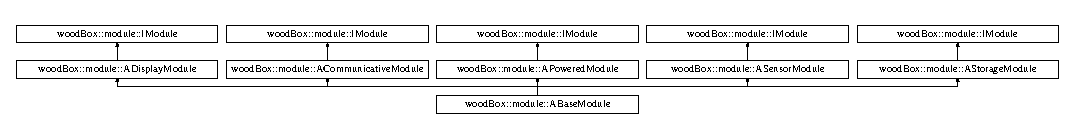
\includegraphics[height=3.000000cm]{classwood_box_1_1module_1_1_a_base_module}
\end{center}
\end{figure}
\subsection*{Public Member Functions}
\begin{DoxyCompactItemize}
\item 
\mbox{\Hypertarget{classwood_box_1_1module_1_1_a_base_module_a61e8f78a69b3ea735e70a13f6de8d662}\label{classwood_box_1_1module_1_1_a_base_module_a61e8f78a69b3ea735e70a13f6de8d662}} 
\mbox{\hyperlink{classwood_box_1_1module_1_1_a_base_module}{A\+Base\+Module}} \& {\bfseries operator=} (\mbox{\hyperlink{classwood_box_1_1module_1_1_a_base_module}{A\+Base\+Module}} \&)=delete
\item 
Stream $\ast$$\ast$ \mbox{\hyperlink{classwood_box_1_1module_1_1_a_base_module_ada9df5e73cb0aee0bada1de17de19a9c}{get\+Streams}} ()
\item 
void \mbox{\hyperlink{classwood_box_1_1module_1_1_a_base_module_a6e3b73bd36f668f5d621dee3070c131a}{set\+Streams}} (Stream $\ast$$\ast$)
\item 
\mbox{\hyperlink{classwood_box_1_1display_1_1_i_display}{display\+::\+I\+Display}} $\ast$ \mbox{\hyperlink{classwood_box_1_1module_1_1_a_base_module_afecd89a2ed85517a6d72ad2f03ea87c3}{get\+Display}} ()
\item 
void \mbox{\hyperlink{classwood_box_1_1module_1_1_a_base_module_a7e99b7d8d59953a8350e9859a475bc6a}{set\+Display}} (\mbox{\hyperlink{classwood_box_1_1display_1_1_i_display}{display\+::\+I\+Display}} $\ast$)
\item 
\mbox{\hyperlink{classwood_box_1_1power_1_1_i_power}{power\+::\+I\+Power}} $\ast$ \mbox{\hyperlink{classwood_box_1_1module_1_1_a_base_module_a1d67c7b9560b30774878e5b882c4bf0a}{get\+Power\+Source}} ()
\item 
void \mbox{\hyperlink{classwood_box_1_1module_1_1_a_base_module_a117ce9fbbcef048ccde38f0b6a11aa91}{set\+Power\+Source}} (\mbox{\hyperlink{classwood_box_1_1power_1_1_i_power}{power\+::\+I\+Power}} $\ast$)
\item 
\mbox{\hyperlink{classwood_box_1_1sensor_1_1_i_sensor}{sensor\+::\+I\+Sensor}} $\ast$ \mbox{\hyperlink{classwood_box_1_1module_1_1_a_base_module_acd7e95a20964a1f9ce2dbbbf629fe3dc}{get\+Sensor}} ()
\item 
void \mbox{\hyperlink{classwood_box_1_1module_1_1_a_base_module_ac3fd88feae532ca88b14642f76ef8def}{set\+Sensor}} (\mbox{\hyperlink{classwood_box_1_1sensor_1_1_i_sensor}{sensor\+::\+I\+Sensor}} $\ast$)
\item 
\mbox{\hyperlink{classwood_box_1_1storage_1_1_i_storage}{storage\+::\+I\+Storage}} $\ast$ \mbox{\hyperlink{classwood_box_1_1module_1_1_a_base_module_ad55a3509dc2bcb2fc5c8abc4a4db1cf1}{get\+Storage}} ()
\item 
void \mbox{\hyperlink{classwood_box_1_1module_1_1_a_base_module_af9e009af37d04062c2da7d977baded80}{set\+Storage}} (\mbox{\hyperlink{classwood_box_1_1storage_1_1_i_storage}{storage\+::\+I\+Storage}} $\ast$)
\end{DoxyCompactItemize}
\subsection*{Protected Member Functions}
\begin{DoxyCompactItemize}
\item 
\mbox{\Hypertarget{classwood_box_1_1module_1_1_a_base_module_a40edd799ba7342abfaf5cb06e60a4b04}\label{classwood_box_1_1module_1_1_a_base_module_a40edd799ba7342abfaf5cb06e60a4b04}} 
{\bfseries A\+Base\+Module} (\mbox{\hyperlink{classwood_box_1_1display_1_1_i_display}{display\+::\+I\+Display}} $\ast$=nullptr, Stream $\ast$$\ast$=nullptr, \mbox{\hyperlink{classwood_box_1_1power_1_1_i_power}{power\+::\+I\+Power}} $\ast$=nullptr, \mbox{\hyperlink{classwood_box_1_1sensor_1_1_i_sensor}{sensor\+::\+I\+Sensor}} $\ast$=nullptr, \mbox{\hyperlink{classwood_box_1_1storage_1_1_i_storage}{storage\+::\+I\+Storage}} $\ast$=nullptr)
\item 
\mbox{\Hypertarget{classwood_box_1_1module_1_1_a_base_module_a2ba8fdaace63960a0696b77bee60b64b}\label{classwood_box_1_1module_1_1_a_base_module_a2ba8fdaace63960a0696b77bee60b64b}} 
{\bfseries A\+Base\+Module} (\mbox{\hyperlink{classwood_box_1_1module_1_1_a_base_module}{A\+Base\+Module}} \&)=delete
\end{DoxyCompactItemize}
\subsection*{Protected Attributes}
\begin{DoxyCompactItemize}
\item 
\mbox{\Hypertarget{classwood_box_1_1module_1_1_a_base_module_a2550178f6fe0a97025e87da03a47d13f}\label{classwood_box_1_1module_1_1_a_base_module_a2550178f6fe0a97025e87da03a47d13f}} 
\mbox{\hyperlink{classwood_box_1_1display_1_1_i_display}{display\+::\+I\+Display}} $\ast$ {\bfseries \+\_\+display}
\item 
\mbox{\Hypertarget{classwood_box_1_1module_1_1_a_base_module_a851b365cdd36435e017297fcfdb8d5e8}\label{classwood_box_1_1module_1_1_a_base_module_a851b365cdd36435e017297fcfdb8d5e8}} 
Stream $\ast$$\ast$ {\bfseries \+\_\+streams}
\item 
\mbox{\Hypertarget{classwood_box_1_1module_1_1_a_base_module_a24c92fcd213167f9f917d6637a8df370}\label{classwood_box_1_1module_1_1_a_base_module_a24c92fcd213167f9f917d6637a8df370}} 
\mbox{\hyperlink{classwood_box_1_1power_1_1_i_power}{power\+::\+I\+Power}} $\ast$ {\bfseries \+\_\+power}
\item 
\mbox{\Hypertarget{classwood_box_1_1module_1_1_a_base_module_a9735d9e5169f0d26c2a9cf2fad3f12a5}\label{classwood_box_1_1module_1_1_a_base_module_a9735d9e5169f0d26c2a9cf2fad3f12a5}} 
\mbox{\hyperlink{classwood_box_1_1sensor_1_1_i_sensor}{sensor\+::\+I\+Sensor}} $\ast$ {\bfseries \+\_\+sensor}
\item 
\mbox{\Hypertarget{classwood_box_1_1module_1_1_a_base_module_aa187748e43497da9786e37c777948901}\label{classwood_box_1_1module_1_1_a_base_module_aa187748e43497da9786e37c777948901}} 
\mbox{\hyperlink{classwood_box_1_1storage_1_1_i_storage}{storage\+::\+I\+Storage}} $\ast$ {\bfseries \+\_\+storage}
\end{DoxyCompactItemize}


\subsection{Detailed Description}
Abstract base class for all Module classes, mainly handling low level logic and accessers to Module components 

\subsection{Member Function Documentation}
\mbox{\Hypertarget{classwood_box_1_1module_1_1_a_base_module_afecd89a2ed85517a6d72ad2f03ea87c3}\label{classwood_box_1_1module_1_1_a_base_module_afecd89a2ed85517a6d72ad2f03ea87c3}} 
\index{wood\+Box\+::module\+::\+A\+Base\+Module@{wood\+Box\+::module\+::\+A\+Base\+Module}!get\+Display@{get\+Display}}
\index{get\+Display@{get\+Display}!wood\+Box\+::module\+::\+A\+Base\+Module@{wood\+Box\+::module\+::\+A\+Base\+Module}}
\subsubsection{\texorpdfstring{get\+Display()}{getDisplay()}}
{\footnotesize\ttfamily \mbox{\hyperlink{classwood_box_1_1display_1_1_i_display}{display\+::\+I\+Display}} $\ast$ wood\+Box\+::module\+::\+A\+Base\+Module\+::get\+Display (\begin{DoxyParamCaption}{ }\end{DoxyParamCaption})}

Return a \mbox{\hyperlink{classwood_box_1_1display_1_1_i_display}{wood\+Box\+::display\+::\+I\+Display}} interface pointer on the display currently used by the module.

Warning\+: On some embedded targets there\textquotesingle{}s no C++ runtime (so no {\ttfamily dynamic\+\_\+cast} or {\ttfamily typeof}), the user will have to know and cast by himself this pointer to the correct type.

If there\textquotesingle{}s no display interface currently used by the module, this method returns {\ttfamily nullptr}. \mbox{\Hypertarget{classwood_box_1_1module_1_1_a_base_module_a1d67c7b9560b30774878e5b882c4bf0a}\label{classwood_box_1_1module_1_1_a_base_module_a1d67c7b9560b30774878e5b882c4bf0a}} 
\index{wood\+Box\+::module\+::\+A\+Base\+Module@{wood\+Box\+::module\+::\+A\+Base\+Module}!get\+Power\+Source@{get\+Power\+Source}}
\index{get\+Power\+Source@{get\+Power\+Source}!wood\+Box\+::module\+::\+A\+Base\+Module@{wood\+Box\+::module\+::\+A\+Base\+Module}}
\subsubsection{\texorpdfstring{get\+Power\+Source()}{getPowerSource()}}
{\footnotesize\ttfamily \mbox{\hyperlink{classwood_box_1_1power_1_1_i_power}{power\+::\+I\+Power}} $\ast$ wood\+Box\+::module\+::\+A\+Base\+Module\+::get\+Power\+Source (\begin{DoxyParamCaption}{ }\end{DoxyParamCaption})}

Return a \mbox{\hyperlink{classwood_box_1_1power_1_1_i_power}{wood\+Box\+::power\+::\+I\+Power}} interface pointer on the power supply currently used by the module.

Warning\+: On some embedded targets there\textquotesingle{}s no C++ runtime (so no {\ttfamily dynamic\+\_\+cast} or {\ttfamily typeof}), the user will have to know and cast by himself this pointer to the correct type.

If there\textquotesingle{}s no power interface currently used by the module, this method returns {\ttfamily nullptr}. \mbox{\Hypertarget{classwood_box_1_1module_1_1_a_base_module_acd7e95a20964a1f9ce2dbbbf629fe3dc}\label{classwood_box_1_1module_1_1_a_base_module_acd7e95a20964a1f9ce2dbbbf629fe3dc}} 
\index{wood\+Box\+::module\+::\+A\+Base\+Module@{wood\+Box\+::module\+::\+A\+Base\+Module}!get\+Sensor@{get\+Sensor}}
\index{get\+Sensor@{get\+Sensor}!wood\+Box\+::module\+::\+A\+Base\+Module@{wood\+Box\+::module\+::\+A\+Base\+Module}}
\subsubsection{\texorpdfstring{get\+Sensor()}{getSensor()}}
{\footnotesize\ttfamily \mbox{\hyperlink{classwood_box_1_1sensor_1_1_i_sensor}{sensor\+::\+I\+Sensor}} $\ast$ wood\+Box\+::module\+::\+A\+Base\+Module\+::get\+Sensor (\begin{DoxyParamCaption}{ }\end{DoxyParamCaption})}

Return a \mbox{\hyperlink{classwood_box_1_1sensor_1_1_i_sensor}{wood\+Box\+::sensor\+::\+I\+Sensor}} interface pointer on the sensor currently used by the module.

Warning\+: On some embedded targets there\textquotesingle{}s no C++ runtime (so no {\ttfamily dynamic\+\_\+cast} or {\ttfamily typeof}), the user will have to know and cast by himself this pointer to the correct type.

If there\textquotesingle{}s no sensor interface currently used by the module, this method returns {\ttfamily nullptr}. \mbox{\Hypertarget{classwood_box_1_1module_1_1_a_base_module_ad55a3509dc2bcb2fc5c8abc4a4db1cf1}\label{classwood_box_1_1module_1_1_a_base_module_ad55a3509dc2bcb2fc5c8abc4a4db1cf1}} 
\index{wood\+Box\+::module\+::\+A\+Base\+Module@{wood\+Box\+::module\+::\+A\+Base\+Module}!get\+Storage@{get\+Storage}}
\index{get\+Storage@{get\+Storage}!wood\+Box\+::module\+::\+A\+Base\+Module@{wood\+Box\+::module\+::\+A\+Base\+Module}}
\subsubsection{\texorpdfstring{get\+Storage()}{getStorage()}}
{\footnotesize\ttfamily \mbox{\hyperlink{classwood_box_1_1storage_1_1_i_storage}{storage\+::\+I\+Storage}} $\ast$ wood\+Box\+::module\+::\+A\+Base\+Module\+::get\+Storage (\begin{DoxyParamCaption}{ }\end{DoxyParamCaption})}

Return a \mbox{\hyperlink{classwood_box_1_1storage_1_1_i_storage}{wood\+Box\+::storage\+::\+I\+Storage}} interface pointer on the storage currently used by the module.

Warning\+: On some embedded targets there\textquotesingle{}s no C++ runtime (so no {\ttfamily dynamic\+\_\+cast} or {\ttfamily typeof}), the user will have to know and cast by himself this pointer to the correct type.

If there\textquotesingle{}s no storage interface currently used by the module, this method returns {\ttfamily nullptr}. \mbox{\Hypertarget{classwood_box_1_1module_1_1_a_base_module_ada9df5e73cb0aee0bada1de17de19a9c}\label{classwood_box_1_1module_1_1_a_base_module_ada9df5e73cb0aee0bada1de17de19a9c}} 
\index{wood\+Box\+::module\+::\+A\+Base\+Module@{wood\+Box\+::module\+::\+A\+Base\+Module}!get\+Streams@{get\+Streams}}
\index{get\+Streams@{get\+Streams}!wood\+Box\+::module\+::\+A\+Base\+Module@{wood\+Box\+::module\+::\+A\+Base\+Module}}
\subsubsection{\texorpdfstring{get\+Streams()}{getStreams()}}
{\footnotesize\ttfamily Stream $\ast$$\ast$ wood\+Box\+::module\+::\+A\+Base\+Module\+::get\+Streams (\begin{DoxyParamCaption}{ }\end{DoxyParamCaption})}

Return an array of pointers on {\ttfamily Stream} derived objects terminated by a {\ttfamily nullptr}.

For example, the array can be like this\+: {\ttfamily \{\&Serial, \&Serial1, \&\mbox{\hyperlink{classwood_box_1_1communication_1_1wifi_1_1_e_s_p8266_wi_fi_communicator}{wood\+Box\+::communication\+::wifi\+::\+E\+S\+P8266\+Wi\+Fi\+Communicator}}, nullptr\}}

If there\textquotesingle{}s no {\ttfamily Stream}s used by the module, this method returns {\ttfamily nullptr} \mbox{\Hypertarget{classwood_box_1_1module_1_1_a_base_module_a7e99b7d8d59953a8350e9859a475bc6a}\label{classwood_box_1_1module_1_1_a_base_module_a7e99b7d8d59953a8350e9859a475bc6a}} 
\index{wood\+Box\+::module\+::\+A\+Base\+Module@{wood\+Box\+::module\+::\+A\+Base\+Module}!set\+Display@{set\+Display}}
\index{set\+Display@{set\+Display}!wood\+Box\+::module\+::\+A\+Base\+Module@{wood\+Box\+::module\+::\+A\+Base\+Module}}
\subsubsection{\texorpdfstring{set\+Display()}{setDisplay()}}
{\footnotesize\ttfamily void wood\+Box\+::module\+::\+A\+Base\+Module\+::set\+Display (\begin{DoxyParamCaption}\item[{\mbox{\hyperlink{classwood_box_1_1display_1_1_i_display}{display\+::\+I\+Display}} $\ast$}]{display }\end{DoxyParamCaption})}

Set the pointer on the \mbox{\hyperlink{classwood_box_1_1display_1_1_i_display}{wood\+Box\+::display\+::\+I\+Display}} interface used by the module. \mbox{\Hypertarget{classwood_box_1_1module_1_1_a_base_module_a117ce9fbbcef048ccde38f0b6a11aa91}\label{classwood_box_1_1module_1_1_a_base_module_a117ce9fbbcef048ccde38f0b6a11aa91}} 
\index{wood\+Box\+::module\+::\+A\+Base\+Module@{wood\+Box\+::module\+::\+A\+Base\+Module}!set\+Power\+Source@{set\+Power\+Source}}
\index{set\+Power\+Source@{set\+Power\+Source}!wood\+Box\+::module\+::\+A\+Base\+Module@{wood\+Box\+::module\+::\+A\+Base\+Module}}
\subsubsection{\texorpdfstring{set\+Power\+Source()}{setPowerSource()}}
{\footnotesize\ttfamily void wood\+Box\+::module\+::\+A\+Base\+Module\+::set\+Power\+Source (\begin{DoxyParamCaption}\item[{\mbox{\hyperlink{classwood_box_1_1power_1_1_i_power}{power\+::\+I\+Power}} $\ast$}]{power }\end{DoxyParamCaption})}

Set the pointer on the \mbox{\hyperlink{classwood_box_1_1power_1_1_i_power}{wood\+Box\+::power\+::\+I\+Power}} interface used by the module. \mbox{\Hypertarget{classwood_box_1_1module_1_1_a_base_module_ac3fd88feae532ca88b14642f76ef8def}\label{classwood_box_1_1module_1_1_a_base_module_ac3fd88feae532ca88b14642f76ef8def}} 
\index{wood\+Box\+::module\+::\+A\+Base\+Module@{wood\+Box\+::module\+::\+A\+Base\+Module}!set\+Sensor@{set\+Sensor}}
\index{set\+Sensor@{set\+Sensor}!wood\+Box\+::module\+::\+A\+Base\+Module@{wood\+Box\+::module\+::\+A\+Base\+Module}}
\subsubsection{\texorpdfstring{set\+Sensor()}{setSensor()}}
{\footnotesize\ttfamily void wood\+Box\+::module\+::\+A\+Base\+Module\+::set\+Sensor (\begin{DoxyParamCaption}\item[{\mbox{\hyperlink{classwood_box_1_1sensor_1_1_i_sensor}{sensor\+::\+I\+Sensor}} $\ast$}]{sensor }\end{DoxyParamCaption})}

Set the pointer on the \mbox{\hyperlink{classwood_box_1_1sensor_1_1_i_sensor}{wood\+Box\+::sensor\+::\+I\+Sensor}} interface used by the module. \mbox{\Hypertarget{classwood_box_1_1module_1_1_a_base_module_af9e009af37d04062c2da7d977baded80}\label{classwood_box_1_1module_1_1_a_base_module_af9e009af37d04062c2da7d977baded80}} 
\index{wood\+Box\+::module\+::\+A\+Base\+Module@{wood\+Box\+::module\+::\+A\+Base\+Module}!set\+Storage@{set\+Storage}}
\index{set\+Storage@{set\+Storage}!wood\+Box\+::module\+::\+A\+Base\+Module@{wood\+Box\+::module\+::\+A\+Base\+Module}}
\subsubsection{\texorpdfstring{set\+Storage()}{setStorage()}}
{\footnotesize\ttfamily void wood\+Box\+::module\+::\+A\+Base\+Module\+::set\+Storage (\begin{DoxyParamCaption}\item[{\mbox{\hyperlink{classwood_box_1_1storage_1_1_i_storage}{storage\+::\+I\+Storage}} $\ast$}]{storage }\end{DoxyParamCaption})}

Set the pointer on the \mbox{\hyperlink{classwood_box_1_1storage_1_1_i_storage}{wood\+Box\+::storage\+::\+I\+Storage}} interface used by the module. \mbox{\Hypertarget{classwood_box_1_1module_1_1_a_base_module_a6e3b73bd36f668f5d621dee3070c131a}\label{classwood_box_1_1module_1_1_a_base_module_a6e3b73bd36f668f5d621dee3070c131a}} 
\index{wood\+Box\+::module\+::\+A\+Base\+Module@{wood\+Box\+::module\+::\+A\+Base\+Module}!set\+Streams@{set\+Streams}}
\index{set\+Streams@{set\+Streams}!wood\+Box\+::module\+::\+A\+Base\+Module@{wood\+Box\+::module\+::\+A\+Base\+Module}}
\subsubsection{\texorpdfstring{set\+Streams()}{setStreams()}}
{\footnotesize\ttfamily void wood\+Box\+::module\+::\+A\+Base\+Module\+::set\+Streams (\begin{DoxyParamCaption}\item[{Stream $\ast$$\ast$}]{streams }\end{DoxyParamCaption})}

Set the array of pointers on Stream derived objects used by module for communications.

For example\+: {\ttfamily Stream $\ast$my\+\_\+array\mbox{[}\mbox{]} = \{\&Serial, \&Serial1, \&\mbox{\hyperlink{classwood_box_1_1communication_1_1wifi_1_1_e_s_p8266_wi_fi_communicator}{wood\+Box\+::communication\+::wifi\+::\+E\+S\+P8266\+Wi\+Fi\+Communicator}}, nullptr\};} 

The documentation for this class was generated from the following files\+:\begin{DoxyCompactItemize}
\item 
A\+Base\+Module.\+hpp\item 
A\+Base\+Module.\+cpp\end{DoxyCompactItemize}

\hypertarget{classwood_box_1_1utility_1_1_a_iterable}{}\section{wood\+Box\+:\+:utility\+:\+:A\+Iterable$<$ T $>$ Class Template Reference}
\label{classwood_box_1_1utility_1_1_a_iterable}\index{wood\+Box\+::utility\+::\+A\+Iterable$<$ T $>$@{wood\+Box\+::utility\+::\+A\+Iterable$<$ T $>$}}
Inheritance diagram for wood\+Box\+:\+:utility\+:\+:A\+Iterable$<$ T $>$\+:\begin{figure}[H]
\begin{center}
\leavevmode
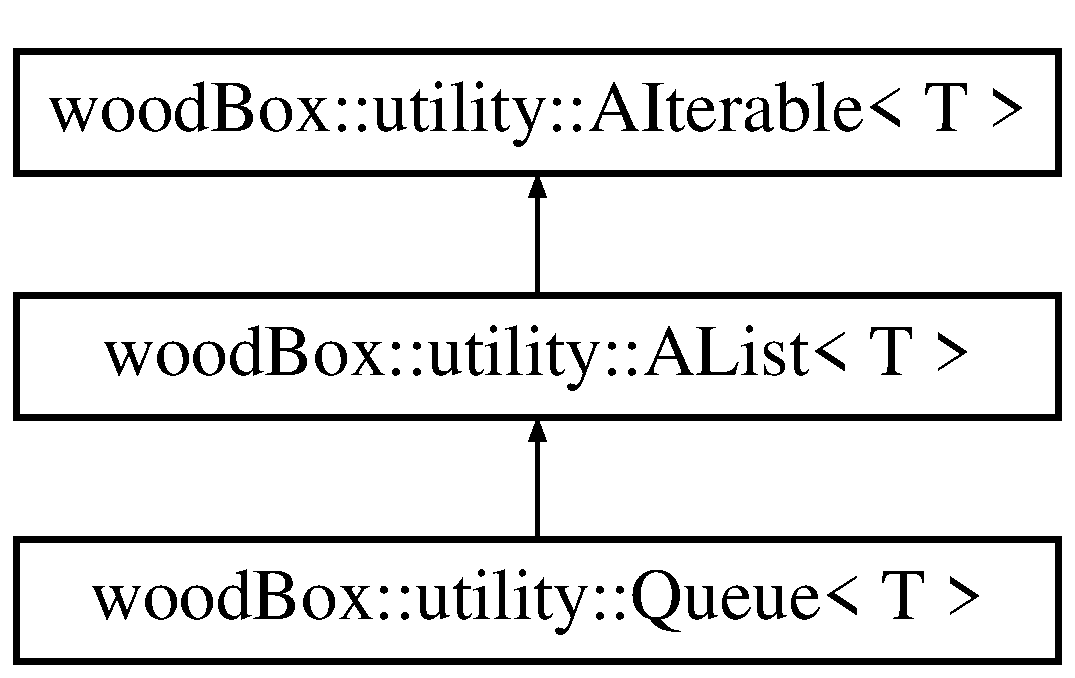
\includegraphics[height=3.000000cm]{classwood_box_1_1utility_1_1_a_iterable}
\end{center}
\end{figure}
\subsection*{Public Member Functions}
\begin{DoxyCompactItemize}
\item 
\mbox{\Hypertarget{classwood_box_1_1utility_1_1_a_iterable_aa8f6eb12adefa838343af8d8854ac7f6}\label{classwood_box_1_1utility_1_1_a_iterable_aa8f6eb12adefa838343af8d8854ac7f6}} 
{\bfseries A\+Iterable} (const \mbox{\hyperlink{classwood_box_1_1utility_1_1_a_iterable}{A\+Iterable}} \&other)=delete
\item 
\mbox{\Hypertarget{classwood_box_1_1utility_1_1_a_iterable_a9dfe1e1906628ef0892b50d12ba8696a}\label{classwood_box_1_1utility_1_1_a_iterable_a9dfe1e1906628ef0892b50d12ba8696a}} 
\mbox{\hyperlink{classwood_box_1_1utility_1_1_a_iterable}{A\+Iterable}} \& {\bfseries operator=} (const \mbox{\hyperlink{classwood_box_1_1utility_1_1_a_iterable}{A\+Iterable}} \&other)=delete
\item 
\mbox{\Hypertarget{classwood_box_1_1utility_1_1_a_iterable_a1ae4da148f184a6e95649c2e967389aa}\label{classwood_box_1_1utility_1_1_a_iterable_a1ae4da148f184a6e95649c2e967389aa}} 
T $\ast$ {\bfseries get} ()
\item 
\mbox{\Hypertarget{classwood_box_1_1utility_1_1_a_iterable_a675dfb37558f14704afeb50ab544f99f}\label{classwood_box_1_1utility_1_1_a_iterable_a675dfb37558f14704afeb50ab544f99f}} 
const T $\ast$ {\bfseries get} () const
\item 
\mbox{\Hypertarget{classwood_box_1_1utility_1_1_a_iterable_ae8978938416061fcfa2180ba2cd7f48c}\label{classwood_box_1_1utility_1_1_a_iterable_ae8978938416061fcfa2180ba2cd7f48c}} 
void {\bfseries set} (T $\ast$data)
\item 
\mbox{\Hypertarget{classwood_box_1_1utility_1_1_a_iterable_a3ddc252101ff34784456f0a3d712f4df}\label{classwood_box_1_1utility_1_1_a_iterable_a3ddc252101ff34784456f0a3d712f4df}} 
virtual \mbox{\hyperlink{classwood_box_1_1utility_1_1_a_iterable}{A\+Iterable}} $\ast$ {\bfseries next} ()=0
\item 
\mbox{\Hypertarget{classwood_box_1_1utility_1_1_a_iterable_a7d3afa98e4226f54e5b9671adec5d0ae}\label{classwood_box_1_1utility_1_1_a_iterable_a7d3afa98e4226f54e5b9671adec5d0ae}} 
virtual const \mbox{\hyperlink{classwood_box_1_1utility_1_1_a_iterable}{A\+Iterable}} $\ast$ {\bfseries next} () const =0
\end{DoxyCompactItemize}
\subsection*{Protected Member Functions}
\begin{DoxyCompactItemize}
\item 
\mbox{\Hypertarget{classwood_box_1_1utility_1_1_a_iterable_a9db8d4d69d94a3e0f230a6f9e8118c20}\label{classwood_box_1_1utility_1_1_a_iterable_a9db8d4d69d94a3e0f230a6f9e8118c20}} 
{\bfseries A\+Iterable} (T $\ast$data=nullptr)
\end{DoxyCompactItemize}


The documentation for this class was generated from the following file\+:\begin{DoxyCompactItemize}
\item 
A\+Iterable.\+hpp\end{DoxyCompactItemize}

\hypertarget{classwood_box_1_1utility_1_1_a_list}{}\section{wood\+Box\+:\+:utility\+:\+:A\+List$<$ T $>$ Class Template Reference}
\label{classwood_box_1_1utility_1_1_a_list}\index{wood\+Box\+::utility\+::\+A\+List$<$ T $>$@{wood\+Box\+::utility\+::\+A\+List$<$ T $>$}}


{\ttfamily \#include $<$A\+List.\+hpp$>$}

Inheritance diagram for wood\+Box\+:\+:utility\+:\+:A\+List$<$ T $>$\+:\begin{figure}[H]
\begin{center}
\leavevmode
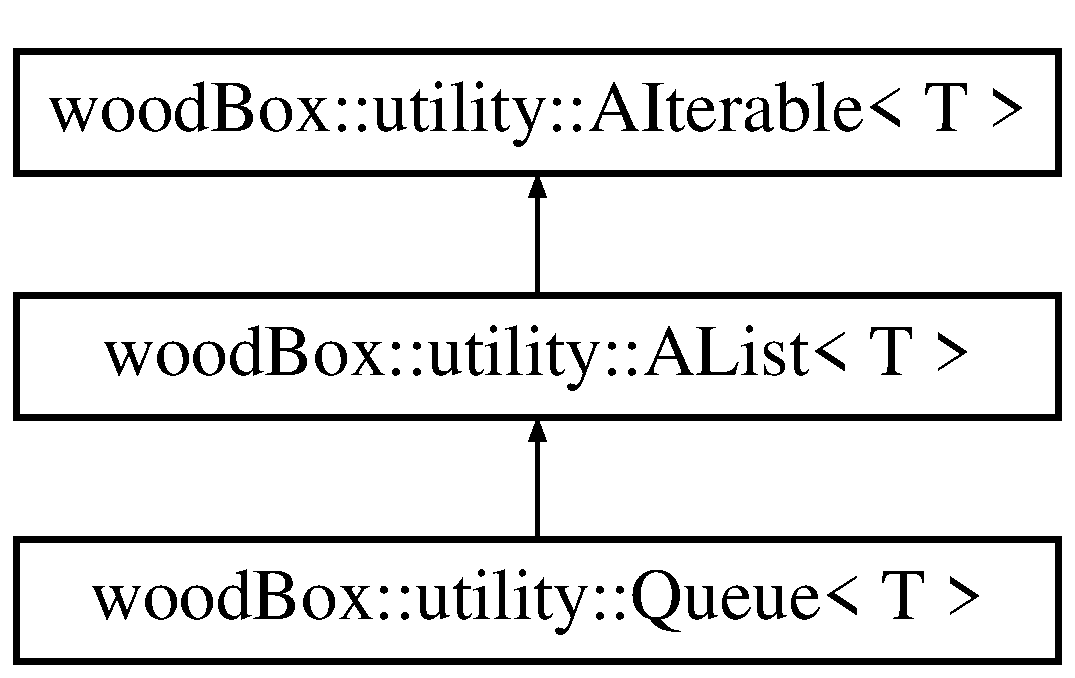
\includegraphics[height=3.000000cm]{classwood_box_1_1utility_1_1_a_list}
\end{center}
\end{figure}
\subsection*{Public Member Functions}
\begin{DoxyCompactItemize}
\item 
\mbox{\Hypertarget{classwood_box_1_1utility_1_1_a_list_a30c716d7e6462759801d1d3009ed5d13}\label{classwood_box_1_1utility_1_1_a_list_a30c716d7e6462759801d1d3009ed5d13}} 
\mbox{\hyperlink{classwood_box_1_1utility_1_1_a_list}{A\+List}} \& {\bfseries operator=} (const \mbox{\hyperlink{classwood_box_1_1utility_1_1_a_list}{A\+List}} \&other)=delete
\item 
\mbox{\Hypertarget{classwood_box_1_1utility_1_1_a_list_ae899fa889dc8909ee9cdffb2cdb0d2b4}\label{classwood_box_1_1utility_1_1_a_list_ae899fa889dc8909ee9cdffb2cdb0d2b4}} 
{\bfseries A\+List} (const \mbox{\hyperlink{classwood_box_1_1utility_1_1_a_list}{A\+List}} \&other)=delete
\item 
\mbox{\Hypertarget{classwood_box_1_1utility_1_1_a_list_ae3769cd3b298718c827026e8f17a2ece}\label{classwood_box_1_1utility_1_1_a_list_ae3769cd3b298718c827026e8f17a2ece}} 
virtual \mbox{\hyperlink{classwood_box_1_1utility_1_1_a_list}{A\+List}} $\ast$ {\bfseries next} ()
\item 
\mbox{\Hypertarget{classwood_box_1_1utility_1_1_a_list_a39e93ebf127847d1f8e7d99c8aa90c2e}\label{classwood_box_1_1utility_1_1_a_list_a39e93ebf127847d1f8e7d99c8aa90c2e}} 
virtual const \mbox{\hyperlink{classwood_box_1_1utility_1_1_a_list}{A\+List}} $\ast$ {\bfseries next} () const
\end{DoxyCompactItemize}
\subsection*{Protected Member Functions}
\begin{DoxyCompactItemize}
\item 
\mbox{\Hypertarget{classwood_box_1_1utility_1_1_a_list_a333eb2d9fa6833bba6675e2b5964ee4f}\label{classwood_box_1_1utility_1_1_a_list_a333eb2d9fa6833bba6675e2b5964ee4f}} 
{\bfseries A\+List} (\mbox{\hyperlink{classwood_box_1_1utility_1_1_a_list}{A\+List}} $\ast$next=nullptr, T $\ast$data=nullptr)
\item 
\mbox{\Hypertarget{classwood_box_1_1utility_1_1_a_list_adc24a832d3c7446cf1958eb9acfeb49b}\label{classwood_box_1_1utility_1_1_a_list_adc24a832d3c7446cf1958eb9acfeb49b}} 
void {\bfseries append} (\mbox{\hyperlink{classwood_box_1_1utility_1_1_a_list}{A\+List}} \&next)
\end{DoxyCompactItemize}
\subsection*{Protected Attributes}
\begin{DoxyCompactItemize}
\item 
\mbox{\Hypertarget{classwood_box_1_1utility_1_1_a_list_a843caa997ee9f3339b7e2b804acd11b7}\label{classwood_box_1_1utility_1_1_a_list_a843caa997ee9f3339b7e2b804acd11b7}} 
\mbox{\hyperlink{classwood_box_1_1utility_1_1_a_list}{A\+List}}$<$ T $>$ $\ast$ {\bfseries \+\_\+next}
\end{DoxyCompactItemize}


\subsection{Detailed Description}
\subsubsection*{template$<$typename T$>$\newline
class wood\+Box\+::utility\+::\+A\+List$<$ T $>$}

Class created for internal use of this library, but not used right now. Could be removed if considered useless. 

The documentation for this class was generated from the following file\+:\begin{DoxyCompactItemize}
\item 
A\+List.\+hpp\end{DoxyCompactItemize}

\hypertarget{classwood_box_1_1sensor_1_1_analog_sensor}{}\section{wood\+Box\+:\+:sensor\+:\+:Analog\+Sensor Class Reference}
\label{classwood_box_1_1sensor_1_1_analog_sensor}\index{wood\+Box\+::sensor\+::\+Analog\+Sensor@{wood\+Box\+::sensor\+::\+Analog\+Sensor}}
Inheritance diagram for wood\+Box\+:\+:sensor\+:\+:Analog\+Sensor\+:\begin{figure}[H]
\begin{center}
\leavevmode
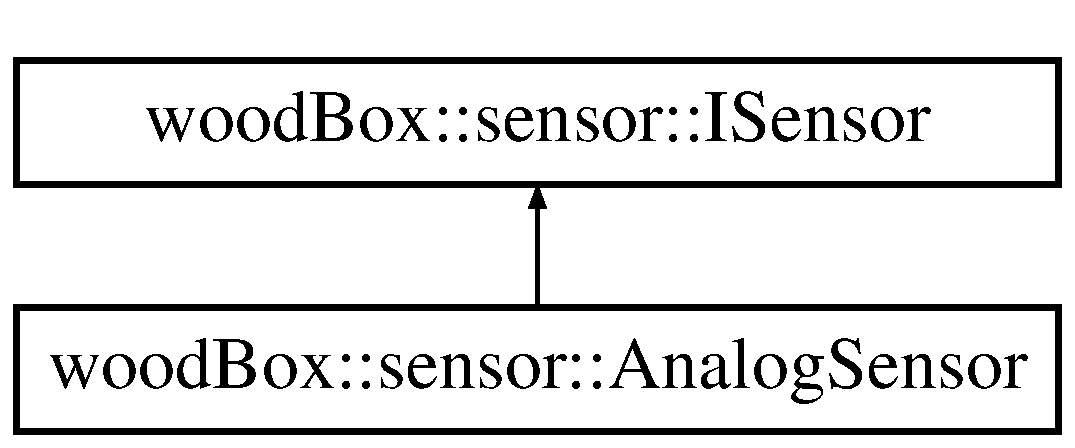
\includegraphics[height=2.000000cm]{classwood_box_1_1sensor_1_1_analog_sensor}
\end{center}
\end{figure}
\subsection*{Public Member Functions}
\begin{DoxyCompactItemize}
\item 
\mbox{\Hypertarget{classwood_box_1_1sensor_1_1_analog_sensor_a41d8ff91cf91d2bdbccffe8f1316421b}\label{classwood_box_1_1sensor_1_1_analog_sensor_a41d8ff91cf91d2bdbccffe8f1316421b}} 
{\bfseries Analog\+Sensor} (uint8\+\_\+t pin)
\item 
\mbox{\Hypertarget{classwood_box_1_1sensor_1_1_analog_sensor_a8ee0238d3fab4515b5286e67f1f92083}\label{classwood_box_1_1sensor_1_1_analog_sensor_a8ee0238d3fab4515b5286e67f1f92083}} 
{\bfseries Analog\+Sensor} (const \mbox{\hyperlink{classwood_box_1_1sensor_1_1_analog_sensor}{Analog\+Sensor}} \&)=delete
\item 
\mbox{\Hypertarget{classwood_box_1_1sensor_1_1_analog_sensor_a66111957aca931c1b1ea219749b03b3c}\label{classwood_box_1_1sensor_1_1_analog_sensor_a66111957aca931c1b1ea219749b03b3c}} 
\mbox{\hyperlink{classwood_box_1_1sensor_1_1_analog_sensor}{Analog\+Sensor}} \& {\bfseries operator=} (const \mbox{\hyperlink{classwood_box_1_1sensor_1_1_analog_sensor}{Analog\+Sensor}} \&)=delete
\item 
virtual uint8\+\_\+t $\ast$ \mbox{\hyperlink{classwood_box_1_1sensor_1_1_analog_sensor_ae78c25d8c01ba9acd03f90f278966189}{get\+Sample}} ()
\item 
virtual \mbox{\hyperlink{classwood_box_1_1sensor_1_1_i_sensor_aa377bda61ed0d4a1d7e1a7bffe459452}{I\+Sensor\+Scale}} \mbox{\hyperlink{classwood_box_1_1sensor_1_1_analog_sensor_a74ddcfe84f3f5b9d7010442f365c4eee}{get\+Estimate}} ()
\item 
\mbox{\Hypertarget{classwood_box_1_1sensor_1_1_analog_sensor_a5a7c67726db40be3edd48294910b117b}\label{classwood_box_1_1sensor_1_1_analog_sensor_a5a7c67726db40be3edd48294910b117b}} 
uint8\+\_\+t {\bfseries get\+Analogue\+Pin} ()
\end{DoxyCompactItemize}
\subsection*{Protected Attributes}
\begin{DoxyCompactItemize}
\item 
\mbox{\Hypertarget{classwood_box_1_1sensor_1_1_analog_sensor_a0377173a16668660f492c52694f96fab}\label{classwood_box_1_1sensor_1_1_analog_sensor_a0377173a16668660f492c52694f96fab}} 
uint8\+\_\+t {\bfseries \+\_\+analog\+\_\+pin}
\end{DoxyCompactItemize}
\subsection*{Additional Inherited Members}


\subsection{Member Function Documentation}
\mbox{\Hypertarget{classwood_box_1_1sensor_1_1_analog_sensor_a74ddcfe84f3f5b9d7010442f365c4eee}\label{classwood_box_1_1sensor_1_1_analog_sensor_a74ddcfe84f3f5b9d7010442f365c4eee}} 
\index{wood\+Box\+::sensor\+::\+Analog\+Sensor@{wood\+Box\+::sensor\+::\+Analog\+Sensor}!get\+Estimate@{get\+Estimate}}
\index{get\+Estimate@{get\+Estimate}!wood\+Box\+::sensor\+::\+Analog\+Sensor@{wood\+Box\+::sensor\+::\+Analog\+Sensor}}
\subsubsection{\texorpdfstring{get\+Estimate()}{getEstimate()}}
{\footnotesize\ttfamily \mbox{\hyperlink{classwood_box_1_1sensor_1_1_i_sensor_aa377bda61ed0d4a1d7e1a7bffe459452}{I\+Sensor\+::\+I\+Sensor\+Scale}} wood\+Box\+::sensor\+::\+Analog\+Sensor\+::get\+Estimate (\begin{DoxyParamCaption}{ }\end{DoxyParamCaption})\hspace{0.3cm}{\ttfamily [virtual]}}

Returns the estimation of safety from the current sensor value 

Implements \mbox{\hyperlink{classwood_box_1_1sensor_1_1_i_sensor_afb01c2473efc4a823bf5dada0048d2bc}{wood\+Box\+::sensor\+::\+I\+Sensor}}.

\mbox{\Hypertarget{classwood_box_1_1sensor_1_1_analog_sensor_ae78c25d8c01ba9acd03f90f278966189}\label{classwood_box_1_1sensor_1_1_analog_sensor_ae78c25d8c01ba9acd03f90f278966189}} 
\index{wood\+Box\+::sensor\+::\+Analog\+Sensor@{wood\+Box\+::sensor\+::\+Analog\+Sensor}!get\+Sample@{get\+Sample}}
\index{get\+Sample@{get\+Sample}!wood\+Box\+::sensor\+::\+Analog\+Sensor@{wood\+Box\+::sensor\+::\+Analog\+Sensor}}
\subsubsection{\texorpdfstring{get\+Sample()}{getSample()}}
{\footnotesize\ttfamily uint8\+\_\+t $\ast$ wood\+Box\+::sensor\+::\+Analog\+Sensor\+::get\+Sample (\begin{DoxyParamCaption}{ }\end{DoxyParamCaption})\hspace{0.3cm}{\ttfamily [virtual]}}

Returns a pointer on sensor sample raw memory, as an array of bytes 

Implements \mbox{\hyperlink{classwood_box_1_1sensor_1_1_i_sensor_a9de8041b991b76cc2f6fcc3b6a1bf363}{wood\+Box\+::sensor\+::\+I\+Sensor}}.



The documentation for this class was generated from the following files\+:\begin{DoxyCompactItemize}
\item 
Analog\+Sensor.\+hpp\item 
Analog\+Sensor.\+cpp\end{DoxyCompactItemize}

\hypertarget{classwood_box_1_1storage_1_1_arduino_e_e_p_r_o_m}{}\section{wood\+Box\+:\+:storage\+:\+:Arduino\+E\+E\+P\+R\+OM Class Reference}
\label{classwood_box_1_1storage_1_1_arduino_e_e_p_r_o_m}\index{wood\+Box\+::storage\+::\+Arduino\+E\+E\+P\+R\+OM@{wood\+Box\+::storage\+::\+Arduino\+E\+E\+P\+R\+OM}}


{\ttfamily \#include $<$Arduino\+E\+E\+P\+R\+O\+M.\+hpp$>$}

Inheritance diagram for wood\+Box\+:\+:storage\+:\+:Arduino\+E\+E\+P\+R\+OM\+:\begin{figure}[H]
\begin{center}
\leavevmode
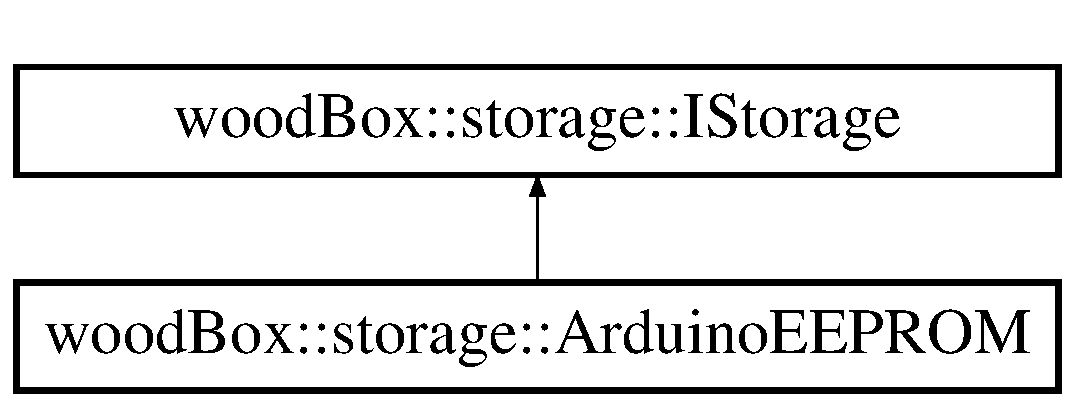
\includegraphics[height=2.000000cm]{classwood_box_1_1storage_1_1_arduino_e_e_p_r_o_m}
\end{center}
\end{figure}
\subsection*{Public Member Functions}
\begin{DoxyCompactItemize}
\item 
\mbox{\Hypertarget{classwood_box_1_1storage_1_1_arduino_e_e_p_r_o_m_aef3abecbf1f622d59dca7d3130292670}\label{classwood_box_1_1storage_1_1_arduino_e_e_p_r_o_m_aef3abecbf1f622d59dca7d3130292670}} 
{\bfseries Arduino\+E\+E\+P\+R\+OM} (const \mbox{\hyperlink{classwood_box_1_1storage_1_1_arduino_e_e_p_r_o_m}{Arduino\+E\+E\+P\+R\+OM}} \&)=delete
\item 
\mbox{\Hypertarget{classwood_box_1_1storage_1_1_arduino_e_e_p_r_o_m_a873dd773954d6813bc5b8005ef2405e3}\label{classwood_box_1_1storage_1_1_arduino_e_e_p_r_o_m_a873dd773954d6813bc5b8005ef2405e3}} 
\mbox{\hyperlink{classwood_box_1_1storage_1_1_arduino_e_e_p_r_o_m}{Arduino\+E\+E\+P\+R\+OM}} \& {\bfseries operator=} (const \mbox{\hyperlink{classwood_box_1_1storage_1_1_arduino_e_e_p_r_o_m}{Arduino\+E\+E\+P\+R\+OM}} \&)=delete
\item 
void \mbox{\hyperlink{classwood_box_1_1storage_1_1_arduino_e_e_p_r_o_m_a1b9deb25ea803456b5450f4e3782fd20}{read}} (size\+\_\+t, void $\ast$, size\+\_\+t)
\item 
void \mbox{\hyperlink{classwood_box_1_1storage_1_1_arduino_e_e_p_r_o_m_af78d2077806af7e1aac65d6890915d77}{write}} (size\+\_\+t, const void $\ast$, size\+\_\+t)
\end{DoxyCompactItemize}


\subsection{Detailed Description}
This class is only available on A\+VR platforms using Arduino, as it is a wrapper of Arduino E\+E\+P\+R\+OM library to implement non-\/volatile storage on A\+VR mcu.

Usage is simple, just create an instance of this object and set is as the storage interface of your module using its set\+Storage method\+:


\begin{DoxyCode}
\textcolor{preprocessor}{#include <woodBox.h>}

ArduinoEEPROM eeprom; \textcolor{comment}{// Create an ArduinoEEPROM instance}
WoodBoxModule<uint16\_t, 15> *module = WoodBoxModule<uint16\_t, 15>::getInstance();

\textcolor{keywordtype}{void} setup() \{
  module->setStorage(&eeprom);
\}

\textcolor{keywordtype}{void} loop() \{
\}
\end{DoxyCode}
 

\subsection{Member Function Documentation}
\mbox{\Hypertarget{classwood_box_1_1storage_1_1_arduino_e_e_p_r_o_m_a1b9deb25ea803456b5450f4e3782fd20}\label{classwood_box_1_1storage_1_1_arduino_e_e_p_r_o_m_a1b9deb25ea803456b5450f4e3782fd20}} 
\index{wood\+Box\+::storage\+::\+Arduino\+E\+E\+P\+R\+OM@{wood\+Box\+::storage\+::\+Arduino\+E\+E\+P\+R\+OM}!read@{read}}
\index{read@{read}!wood\+Box\+::storage\+::\+Arduino\+E\+E\+P\+R\+OM@{wood\+Box\+::storage\+::\+Arduino\+E\+E\+P\+R\+OM}}
\subsubsection{\texorpdfstring{read()}{read()}}
{\footnotesize\ttfamily void wood\+Box\+::storage\+::\+Arduino\+E\+E\+P\+R\+O\+M\+::read (\begin{DoxyParamCaption}\item[{size\+\_\+t}]{offset,  }\item[{void $\ast$}]{dest,  }\item[{size\+\_\+t}]{len }\end{DoxyParamCaption})\hspace{0.3cm}{\ttfamily [virtual]}}

See \mbox{\hyperlink{classwood_box_1_1storage_1_1_i_storage_a01bab924be0844e3866b27279caa506d}{wood\+Box\+::storage\+::\+I\+Storage\+::read}} for method documentation. 

Implements \mbox{\hyperlink{classwood_box_1_1storage_1_1_i_storage_a01bab924be0844e3866b27279caa506d}{wood\+Box\+::storage\+::\+I\+Storage}}.

\mbox{\Hypertarget{classwood_box_1_1storage_1_1_arduino_e_e_p_r_o_m_af78d2077806af7e1aac65d6890915d77}\label{classwood_box_1_1storage_1_1_arduino_e_e_p_r_o_m_af78d2077806af7e1aac65d6890915d77}} 
\index{wood\+Box\+::storage\+::\+Arduino\+E\+E\+P\+R\+OM@{wood\+Box\+::storage\+::\+Arduino\+E\+E\+P\+R\+OM}!write@{write}}
\index{write@{write}!wood\+Box\+::storage\+::\+Arduino\+E\+E\+P\+R\+OM@{wood\+Box\+::storage\+::\+Arduino\+E\+E\+P\+R\+OM}}
\subsubsection{\texorpdfstring{write()}{write()}}
{\footnotesize\ttfamily void wood\+Box\+::storage\+::\+Arduino\+E\+E\+P\+R\+O\+M\+::write (\begin{DoxyParamCaption}\item[{size\+\_\+t}]{offset,  }\item[{const void $\ast$}]{src,  }\item[{size\+\_\+t}]{len }\end{DoxyParamCaption})\hspace{0.3cm}{\ttfamily [virtual]}}

See \mbox{\hyperlink{classwood_box_1_1storage_1_1_i_storage_a5eb82c922e8a3147ddab510706be8e24}{wood\+Box\+::storage\+::\+I\+Storage\+::write}} for method documentation.

Content is written only if stored bytes in the E\+E\+P\+R\+OM are different from the one passed as parameter through the memory pointer, to increase E\+E\+P\+R\+OM lifespan. 

Implements \mbox{\hyperlink{classwood_box_1_1storage_1_1_i_storage_a5eb82c922e8a3147ddab510706be8e24}{wood\+Box\+::storage\+::\+I\+Storage}}.



The documentation for this class was generated from the following files\+:\begin{DoxyCompactItemize}
\item 
Arduino\+E\+E\+P\+R\+O\+M.\+hpp\item 
Arduino\+E\+E\+P\+R\+O\+M.\+cpp\end{DoxyCompactItemize}

\hypertarget{classwood_box_1_1display_1_1_a_r_g_b_led}{}\section{wood\+Box\+:\+:display\+:\+:A\+R\+G\+B\+Led Class Reference}
\label{classwood_box_1_1display_1_1_a_r_g_b_led}\index{wood\+Box\+::display\+::\+A\+R\+G\+B\+Led@{wood\+Box\+::display\+::\+A\+R\+G\+B\+Led}}


{\ttfamily \#include $<$A\+R\+G\+B\+Led.\+hpp$>$}

Inheritance diagram for wood\+Box\+:\+:display\+:\+:A\+R\+G\+B\+Led\+:\begin{figure}[H]
\begin{center}
\leavevmode
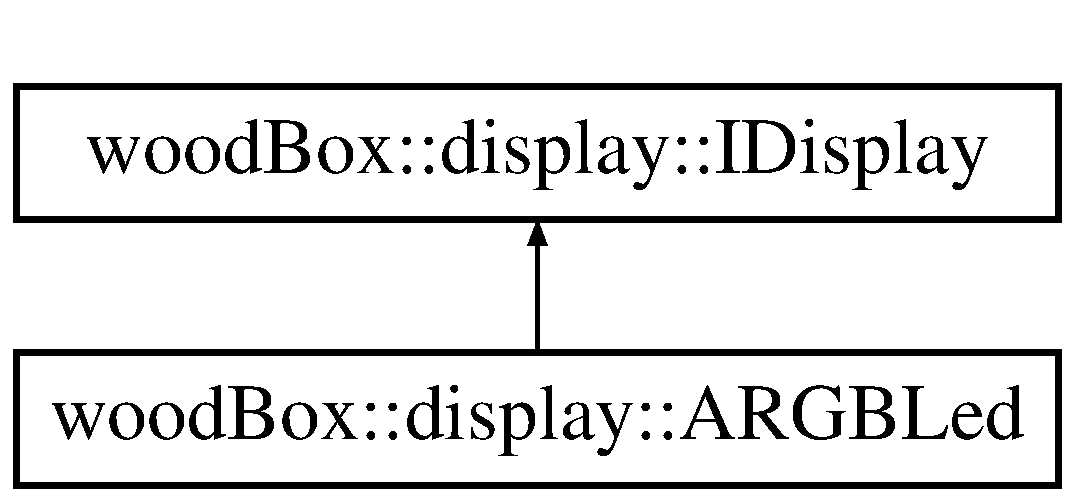
\includegraphics[height=2.121212cm]{classwood_box_1_1display_1_1_a_r_g_b_led}
\end{center}
\end{figure}
\subsection*{Classes}
\begin{DoxyCompactItemize}
\item 
struct \mbox{\hyperlink{structwood_box_1_1display_1_1_a_r_g_b_led_1_1_color}{Color}}
\end{DoxyCompactItemize}
\subsection*{Public Member Functions}
\begin{DoxyCompactItemize}
\item 
\mbox{\Hypertarget{classwood_box_1_1display_1_1_a_r_g_b_led_a9d09c3d236e0ff522f1c4057aee6e3a9}\label{classwood_box_1_1display_1_1_a_r_g_b_led_a9d09c3d236e0ff522f1c4057aee6e3a9}} 
{\bfseries A\+R\+G\+B\+Led} (\mbox{\hyperlink{classwood_box_1_1display_1_1_a_r_g_b_led}{A\+R\+G\+B\+Led}} const \&)=delete
\item 
\mbox{\Hypertarget{classwood_box_1_1display_1_1_a_r_g_b_led_acbc8bea5a3b1fe292d3ac37ab647d21b}\label{classwood_box_1_1display_1_1_a_r_g_b_led_acbc8bea5a3b1fe292d3ac37ab647d21b}} 
\mbox{\hyperlink{classwood_box_1_1display_1_1_a_r_g_b_led}{A\+R\+G\+B\+Led}} \& {\bfseries operator=} (\mbox{\hyperlink{classwood_box_1_1display_1_1_a_r_g_b_led}{A\+R\+G\+B\+Led}} const \&)=delete
\item 
void \mbox{\hyperlink{classwood_box_1_1display_1_1_a_r_g_b_led_a6639eef02bb6b70988d85c006f73eb72}{clear}} ()
\item 
virtual void \mbox{\hyperlink{classwood_box_1_1display_1_1_a_r_g_b_led_ab71f321d91e931f95b96d1f492a9454d}{update}} ()=0
\item 
const \mbox{\hyperlink{structwood_box_1_1display_1_1_a_r_g_b_led_1_1_color}{Color}} \& \mbox{\hyperlink{classwood_box_1_1display_1_1_a_r_g_b_led_ae0bd01eab303006612eb46058824b0c1}{get\+Color}} () const
\item 
void \mbox{\hyperlink{classwood_box_1_1display_1_1_a_r_g_b_led_ac06b3ee90d2f49785173e9142df47bb7}{set\+Color}} (const \mbox{\hyperlink{structwood_box_1_1display_1_1_a_r_g_b_led_1_1_color}{Color}} \&color)
\end{DoxyCompactItemize}


\subsection{Detailed Description}
Abstract class used to control R\+GB L\+E\+Ds (Common cathode/anode, Grove Chainable L\+E\+Ds, Neo\+Pixels, ...etc)

Example of use\+:


\begin{DoxyCode}
\textcolor{keywordtype}{void} my\_function\_changing\_led\_color(ARGBLed &led) \{
  Color red = \{255, 0, 0\}; \textcolor{comment}{// Create a Color structure with red fully on, green off and blue off}
  led.setColor(red); \textcolor{comment}{// Set the new color by calling setColor method}
  led.update(); \textcolor{comment}{// Display the new color on the LED}
\}
\end{DoxyCode}
 

\subsection{Member Function Documentation}
\mbox{\Hypertarget{classwood_box_1_1display_1_1_a_r_g_b_led_a6639eef02bb6b70988d85c006f73eb72}\label{classwood_box_1_1display_1_1_a_r_g_b_led_a6639eef02bb6b70988d85c006f73eb72}} 
\index{wood\+Box\+::display\+::\+A\+R\+G\+B\+Led@{wood\+Box\+::display\+::\+A\+R\+G\+B\+Led}!clear@{clear}}
\index{clear@{clear}!wood\+Box\+::display\+::\+A\+R\+G\+B\+Led@{wood\+Box\+::display\+::\+A\+R\+G\+B\+Led}}
\subsubsection{\texorpdfstring{clear()}{clear()}}
{\footnotesize\ttfamily void wood\+Box\+::display\+::\+A\+R\+G\+B\+Led\+::clear (\begin{DoxyParamCaption}{ }\end{DoxyParamCaption})\hspace{0.3cm}{\ttfamily [inline]}, {\ttfamily [virtual]}}

Remove display content 

Implements \mbox{\hyperlink{classwood_box_1_1display_1_1_i_display_a7030f0768c1ef15ce936a259406168dc}{wood\+Box\+::display\+::\+I\+Display}}.

\mbox{\Hypertarget{classwood_box_1_1display_1_1_a_r_g_b_led_ae0bd01eab303006612eb46058824b0c1}\label{classwood_box_1_1display_1_1_a_r_g_b_led_ae0bd01eab303006612eb46058824b0c1}} 
\index{wood\+Box\+::display\+::\+A\+R\+G\+B\+Led@{wood\+Box\+::display\+::\+A\+R\+G\+B\+Led}!get\+Color@{get\+Color}}
\index{get\+Color@{get\+Color}!wood\+Box\+::display\+::\+A\+R\+G\+B\+Led@{wood\+Box\+::display\+::\+A\+R\+G\+B\+Led}}
\subsubsection{\texorpdfstring{get\+Color()}{getColor()}}
{\footnotesize\ttfamily const \mbox{\hyperlink{structwood_box_1_1display_1_1_a_r_g_b_led_1_1_color}{Color}}\& wood\+Box\+::display\+::\+A\+R\+G\+B\+Led\+::get\+Color (\begin{DoxyParamCaption}{ }\end{DoxyParamCaption}) const\hspace{0.3cm}{\ttfamily [inline]}}

Return a reference on the \mbox{\hyperlink{structwood_box_1_1display_1_1_a_r_g_b_led_1_1_color}{Color}} structure representing the current color displayed (or next color, if L\+ED color hasn\textquotesingle{}t been updated since last change of color made by set\+Color)

Example\+:


\begin{DoxyCode}
\textcolor{keywordtype}{void} my\_function\_printing\_led\_color(\textcolor{keyword}{const} ARGBLed &led) \{
  \textcolor{keyword}{const} Color &color = led.getColor();
\textcolor{preprocessor}{#ifdef ARDUINO}
  Serial.print(\textcolor{stringliteral}{"Red: "});
  Serial.print(led.red);
  Serial.print(\textcolor{stringliteral}{", Green: "});
  Serial.print(led.green);
  Serial.print(\textcolor{stringliteral}{", Blue: "});
  Serial.println(led.blue);
\textcolor{preprocessor}{#else}
  printf(\textcolor{stringliteral}{"Red: %u, Green: %u, Blue: %u\(\backslash\)n"}, led.red, led.green, led.blue);
\textcolor{preprocessor}{#endif}
\textcolor{preprocessor}{\}}
\end{DoxyCode}
 \mbox{\Hypertarget{classwood_box_1_1display_1_1_a_r_g_b_led_ac06b3ee90d2f49785173e9142df47bb7}\label{classwood_box_1_1display_1_1_a_r_g_b_led_ac06b3ee90d2f49785173e9142df47bb7}} 
\index{wood\+Box\+::display\+::\+A\+R\+G\+B\+Led@{wood\+Box\+::display\+::\+A\+R\+G\+B\+Led}!set\+Color@{set\+Color}}
\index{set\+Color@{set\+Color}!wood\+Box\+::display\+::\+A\+R\+G\+B\+Led@{wood\+Box\+::display\+::\+A\+R\+G\+B\+Led}}
\subsubsection{\texorpdfstring{set\+Color()}{setColor()}}
{\footnotesize\ttfamily void wood\+Box\+::display\+::\+A\+R\+G\+B\+Led\+::set\+Color (\begin{DoxyParamCaption}\item[{const \mbox{\hyperlink{structwood_box_1_1display_1_1_a_r_g_b_led_1_1_color}{Color}} \&}]{color }\end{DoxyParamCaption})\hspace{0.3cm}{\ttfamily [inline]}}

Set the new color to display on the L\+ED.

Note\+: You need to call the \char`\"{}update\char`\"{} method after this one, as it doesn\textquotesingle{}t update automatically the new color on the L\+ED.

Example\+:


\begin{DoxyCode}
\textcolor{keyword}{const} Color red = \{255, 0, 0\};

\textcolor{keywordtype}{void} my\_function\_changing\_a\_led\_color\_to\_red(ARGBLed &led) \{
  led.setColor(red); \textcolor{comment}{// Set the new color in the LED object}
  led.update(); \textcolor{comment}{// You need to call this method if you want the new color to be displayed on the LED}
\}
\end{DoxyCode}
 \mbox{\Hypertarget{classwood_box_1_1display_1_1_a_r_g_b_led_ab71f321d91e931f95b96d1f492a9454d}\label{classwood_box_1_1display_1_1_a_r_g_b_led_ab71f321d91e931f95b96d1f492a9454d}} 
\index{wood\+Box\+::display\+::\+A\+R\+G\+B\+Led@{wood\+Box\+::display\+::\+A\+R\+G\+B\+Led}!update@{update}}
\index{update@{update}!wood\+Box\+::display\+::\+A\+R\+G\+B\+Led@{wood\+Box\+::display\+::\+A\+R\+G\+B\+Led}}
\subsubsection{\texorpdfstring{update()}{update()}}
{\footnotesize\ttfamily virtual void wood\+Box\+::display\+::\+A\+R\+G\+B\+Led\+::update (\begin{DoxyParamCaption}{ }\end{DoxyParamCaption})\hspace{0.3cm}{\ttfamily [pure virtual]}}

Update display content 

Implements \mbox{\hyperlink{classwood_box_1_1display_1_1_i_display_ad8c0811b8b807ce119a06c7806004de7}{wood\+Box\+::display\+::\+I\+Display}}.



Implemented in \mbox{\hyperlink{classwood_box_1_1display_1_1_grove_chainable_l_e_d_a650969665d0b5607465a63159c62e4ef}{wood\+Box\+::display\+::\+Grove\+Chainable\+L\+ED}}, \mbox{\hyperlink{classwood_box_1_1display_1_1_neo_pixel_ac2ec48825a10154e0ef99c4d8010aa6e}{wood\+Box\+::display\+::\+Neo\+Pixel}}, and \mbox{\hyperlink{classwood_box_1_1display_1_1_common_cathode_r_g_b_led_a597c7ae002c7f94431ccaafd160a857a}{wood\+Box\+::display\+::\+Common\+Cathode\+R\+G\+B\+Led}}.



The documentation for this class was generated from the following file\+:\begin{DoxyCompactItemize}
\item 
A\+R\+G\+B\+Led.\+hpp\end{DoxyCompactItemize}

\hypertarget{classwood_box_1_1communication_1_1wifi_1_1_a_wi_fi_communicator}{}\section{wood\+Box\+:\+:communication\+:\+:wifi\+:\+:A\+Wi\+Fi\+Communicator Class Reference}
\label{classwood_box_1_1communication_1_1wifi_1_1_a_wi_fi_communicator}\index{wood\+Box\+::communication\+::wifi\+::\+A\+Wi\+Fi\+Communicator@{wood\+Box\+::communication\+::wifi\+::\+A\+Wi\+Fi\+Communicator}}


{\ttfamily \#include $<$A\+Wi\+Fi\+Communicator.\+hpp$>$}

Inheritance diagram for wood\+Box\+:\+:communication\+:\+:wifi\+:\+:A\+Wi\+Fi\+Communicator\+:\begin{figure}[H]
\begin{center}
\leavevmode
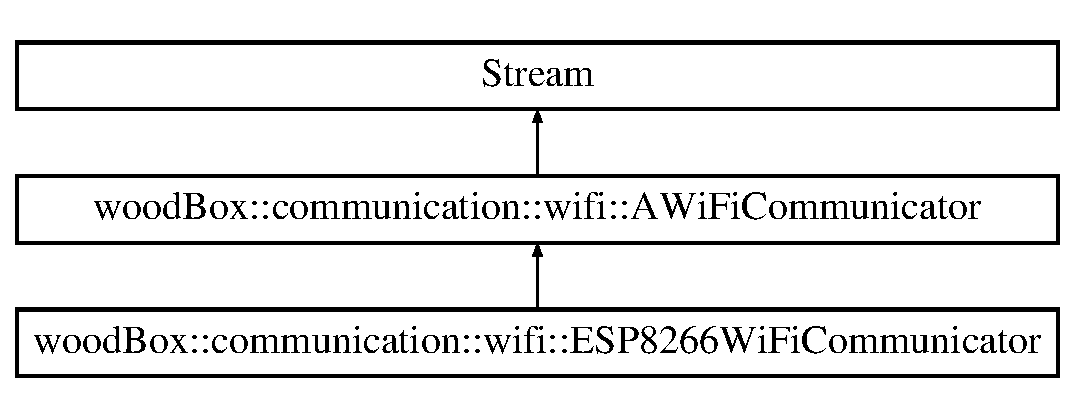
\includegraphics[height=3.000000cm]{classwood_box_1_1communication_1_1wifi_1_1_a_wi_fi_communicator}
\end{center}
\end{figure}
\subsection*{Public Member Functions}
\begin{DoxyCompactItemize}
\item 
\mbox{\hyperlink{classwood_box_1_1communication_1_1wifi_1_1_a_wi_fi_communicator_a9d1dc13ca9243170b04211bef2b86ed2}{A\+Wi\+Fi\+Communicator}} (const \mbox{\hyperlink{structwood_box_1_1communication_1_1wifi_1_1s__wifi__access__point}{Wi\+Fi\+\_\+ap}} $\ast$=nullptr, const \mbox{\hyperlink{structwood_box_1_1communication_1_1wifi_1_1s__wifi__client}{Wi\+Fi\+\_\+client}} $\ast$=nullptr, const wifi\+\_\+mode=S\+T\+A\+T\+I\+ON, Stream $\ast$=nullptr)
\item 
\mbox{\Hypertarget{classwood_box_1_1communication_1_1wifi_1_1_a_wi_fi_communicator_aef6faae3bf738776f0fb437a45c27883}\label{classwood_box_1_1communication_1_1wifi_1_1_a_wi_fi_communicator_aef6faae3bf738776f0fb437a45c27883}} 
{\bfseries A\+Wi\+Fi\+Communicator} (const \mbox{\hyperlink{classwood_box_1_1communication_1_1wifi_1_1_a_wi_fi_communicator}{A\+Wi\+Fi\+Communicator}} \&)=delete
\item 
\mbox{\Hypertarget{classwood_box_1_1communication_1_1wifi_1_1_a_wi_fi_communicator_a9f3c118a4268d09632f483aeb736a7c8}\label{classwood_box_1_1communication_1_1wifi_1_1_a_wi_fi_communicator_a9f3c118a4268d09632f483aeb736a7c8}} 
\mbox{\hyperlink{classwood_box_1_1communication_1_1wifi_1_1_a_wi_fi_communicator}{A\+Wi\+Fi\+Communicator}} \& {\bfseries operator=} (const \mbox{\hyperlink{classwood_box_1_1communication_1_1wifi_1_1_a_wi_fi_communicator}{A\+Wi\+Fi\+Communicator}} \&)=delete
\item 
virtual int \mbox{\hyperlink{classwood_box_1_1communication_1_1wifi_1_1_a_wi_fi_communicator_a541a26bf14cf77c13cc960963944ba1d}{available}} ()=0
\item 
virtual int \mbox{\hyperlink{classwood_box_1_1communication_1_1wifi_1_1_a_wi_fi_communicator_af4bc1adc96c124e769eb8c54d76476cf}{read}} ()=0
\item 
virtual int \mbox{\hyperlink{classwood_box_1_1communication_1_1wifi_1_1_a_wi_fi_communicator_ae0a1f2f1906f76a12dd5f9b7c10b1282}{peek}} ()=0
\item 
virtual size\+\_\+t \mbox{\hyperlink{classwood_box_1_1communication_1_1wifi_1_1_a_wi_fi_communicator_a7c40345fe59737b83bfee33ecb7be013}{write}} (uint8\+\_\+t)=0
\item 
virtual void \mbox{\hyperlink{classwood_box_1_1communication_1_1wifi_1_1_a_wi_fi_communicator_a1c74b8bc27a89604b4b7daa94c0168a6}{flush}} ()=0
\item 
virtual int \mbox{\hyperlink{classwood_box_1_1communication_1_1wifi_1_1_a_wi_fi_communicator_a7c4763c1594a4b934e5a39e90b271799}{connect}} ()=0
\item 
virtual int \mbox{\hyperlink{classwood_box_1_1communication_1_1wifi_1_1_a_wi_fi_communicator_ae0be1e1dd1e0508bdd2f348f0052f6e6}{disconnect}} ()=0
\item 
virtual int \mbox{\hyperlink{classwood_box_1_1communication_1_1wifi_1_1_a_wi_fi_communicator_ad8c31be391a58bfabe21c5ef99a94719}{connect\+To\+Host}} ()=0
\item 
virtual int \mbox{\hyperlink{classwood_box_1_1communication_1_1wifi_1_1_a_wi_fi_communicator_aeb87d8a22ad08c929c28191a4c725a5b}{disconnect\+From\+Host}} ()=0
\item 
virtual bool \mbox{\hyperlink{classwood_box_1_1communication_1_1wifi_1_1_a_wi_fi_communicator_afe42af0100dd483564995b8fc54b2e71}{is\+Connected}} ()=0
\item 
const \mbox{\hyperlink{structwood_box_1_1communication_1_1wifi_1_1s__wifi__access__point}{Wi\+Fi\+\_\+ap}} \& \mbox{\hyperlink{classwood_box_1_1communication_1_1wifi_1_1_a_wi_fi_communicator_abda6749593511b1acc44a999734b9bd6}{get\+Access\+Point}} () const
\item 
\mbox{\Hypertarget{classwood_box_1_1communication_1_1wifi_1_1_a_wi_fi_communicator_a9b0669461151786a0c70fbb1c1a07bc7}\label{classwood_box_1_1communication_1_1wifi_1_1_a_wi_fi_communicator_a9b0669461151786a0c70fbb1c1a07bc7}} 
const \mbox{\hyperlink{structwood_box_1_1communication_1_1wifi_1_1s__wifi__client}{Wi\+Fi\+\_\+client}} \& {\bfseries get\+Connection\+Addresses} () const
\item 
\mbox{\Hypertarget{classwood_box_1_1communication_1_1wifi_1_1_a_wi_fi_communicator_a6bd3193f145df44c577da0f0e7a8686a}\label{classwood_box_1_1communication_1_1wifi_1_1_a_wi_fi_communicator_a6bd3193f145df44c577da0f0e7a8686a}} 
const \mbox{\hyperlink{structwood_box_1_1communication_1_1ip_1_1s__host}{ip\+::tcp\+\_\+host}} \& {\bfseries get\+Host} () const
\item 
\mbox{\Hypertarget{classwood_box_1_1communication_1_1wifi_1_1_a_wi_fi_communicator_aa5b3e64e11585cb4ac16e7bd39fe565b}\label{classwood_box_1_1communication_1_1wifi_1_1_a_wi_fi_communicator_aa5b3e64e11585cb4ac16e7bd39fe565b}} 
wifi\+\_\+mode {\bfseries get\+Wi\+Fi\+Mode} () const
\item 
\mbox{\Hypertarget{classwood_box_1_1communication_1_1wifi_1_1_a_wi_fi_communicator_a6987322a622fab72d4a01de99da19491}\label{classwood_box_1_1communication_1_1wifi_1_1_a_wi_fi_communicator_a6987322a622fab72d4a01de99da19491}} 
void {\bfseries set\+Access\+Point} (const \mbox{\hyperlink{structwood_box_1_1communication_1_1wifi_1_1s__wifi__access__point}{Wi\+Fi\+\_\+ap}} \&)
\item 
\mbox{\Hypertarget{classwood_box_1_1communication_1_1wifi_1_1_a_wi_fi_communicator_ae0e96daf4cbeef3e646cc5af87eaa82d}\label{classwood_box_1_1communication_1_1wifi_1_1_a_wi_fi_communicator_ae0e96daf4cbeef3e646cc5af87eaa82d}} 
void {\bfseries set\+Connection\+Addresses} (const \mbox{\hyperlink{structwood_box_1_1communication_1_1wifi_1_1s__wifi__client}{Wi\+Fi\+\_\+client}} \&)
\item 
\mbox{\Hypertarget{classwood_box_1_1communication_1_1wifi_1_1_a_wi_fi_communicator_a1bbe3367296c647d6846b3c7d0313261}\label{classwood_box_1_1communication_1_1wifi_1_1_a_wi_fi_communicator_a1bbe3367296c647d6846b3c7d0313261}} 
void {\bfseries set\+Host} (const \mbox{\hyperlink{structwood_box_1_1communication_1_1ip_1_1s__host}{ip\+::tcp\+\_\+host}} \&)
\item 
\mbox{\Hypertarget{classwood_box_1_1communication_1_1wifi_1_1_a_wi_fi_communicator_a813fcffda64d86abfe0316a873f23f54}\label{classwood_box_1_1communication_1_1wifi_1_1_a_wi_fi_communicator_a813fcffda64d86abfe0316a873f23f54}} 
void {\bfseries set\+Wi\+Fi\+Mode} (wifi\+\_\+mode)
\item 
\mbox{\Hypertarget{classwood_box_1_1communication_1_1wifi_1_1_a_wi_fi_communicator_a526d2c9ece9000889fd40d9ab98acbdf}\label{classwood_box_1_1communication_1_1wifi_1_1_a_wi_fi_communicator_a526d2c9ece9000889fd40d9ab98acbdf}} 
void {\bfseries set\+Stream\+To\+Chipset} (Stream $\ast$)
\end{DoxyCompactItemize}
\subsection*{Protected Attributes}
\begin{DoxyCompactItemize}
\item 
\mbox{\Hypertarget{classwood_box_1_1communication_1_1wifi_1_1_a_wi_fi_communicator_ac07f090eb75730353a78f2d26f2095f1}\label{classwood_box_1_1communication_1_1wifi_1_1_a_wi_fi_communicator_ac07f090eb75730353a78f2d26f2095f1}} 
wifi\+\_\+mode {\bfseries \+\_\+mode}
\item 
\mbox{\Hypertarget{classwood_box_1_1communication_1_1wifi_1_1_a_wi_fi_communicator_a297970584d8120015f898afa1278eb46}\label{classwood_box_1_1communication_1_1wifi_1_1_a_wi_fi_communicator_a297970584d8120015f898afa1278eb46}} 
Stream $\ast$ {\bfseries \+\_\+stream}
\item 
\mbox{\Hypertarget{classwood_box_1_1communication_1_1wifi_1_1_a_wi_fi_communicator_a9d2cdaede0b5e5040867c3d428dd98f0}\label{classwood_box_1_1communication_1_1wifi_1_1_a_wi_fi_communicator_a9d2cdaede0b5e5040867c3d428dd98f0}} 
\mbox{\hyperlink{structwood_box_1_1communication_1_1wifi_1_1s__wifi__access__point}{Wi\+Fi\+\_\+ap}} {\bfseries \+\_\+ap}
\item 
\mbox{\Hypertarget{classwood_box_1_1communication_1_1wifi_1_1_a_wi_fi_communicator_afde4ef66d5296fbeeff2e1b333105bec}\label{classwood_box_1_1communication_1_1wifi_1_1_a_wi_fi_communicator_afde4ef66d5296fbeeff2e1b333105bec}} 
\mbox{\hyperlink{structwood_box_1_1communication_1_1wifi_1_1s__wifi__client}{Wi\+Fi\+\_\+client}} {\bfseries \+\_\+me}
\item 
\mbox{\Hypertarget{classwood_box_1_1communication_1_1wifi_1_1_a_wi_fi_communicator_ace744bc5d2c8f66dcd735029b129dea6}\label{classwood_box_1_1communication_1_1wifi_1_1_a_wi_fi_communicator_ace744bc5d2c8f66dcd735029b129dea6}} 
\mbox{\hyperlink{structwood_box_1_1communication_1_1ip_1_1s__host}{ip\+::tcp\+\_\+host}} {\bfseries \+\_\+host}
\end{DoxyCompactItemize}


\subsection{Detailed Description}
Abstract class derived from Stream, declaring some new Wi\+Fi common interface methods, and implementing some utility methods for these {\ttfamily Stream}s

Here\textquotesingle{}s a simple example of implementing a U\+A\+RT to Wi\+Fi chipset pre-\/configured to connect a Wi\+Fi network and transparently bridge the serial connection always connected to Serial Stream\+:


\begin{DoxyCode}
\textcolor{preprocessor}{#include <AWiFiCommunicator.hpp>}

\textcolor{keyword}{using} \mbox{\hyperlink{classwood_box_1_1communication_1_1wifi_1_1_a_wi_fi_communicator}{woodBox::communication::wifi::AWiFiCommunicator}};

\textcolor{keyword}{class }MyUARTBridge : \textcolor{keyword}{public} \mbox{\hyperlink{classwood_box_1_1communication_1_1wifi_1_1_a_wi_fi_communicator_a9d1dc13ca9243170b04211bef2b86ed2}{AWiFiCommunicator}} \{
  \textcolor{keyword}{public}:
    MyUARTBridge():\mbox{\hyperlink{classwood_box_1_1communication_1_1wifi_1_1_a_wi_fi_communicator_a9d1dc13ca9243170b04211bef2b86ed2}{AWiFiCommunicator}}() \{
      \_stream = &Serial;
    \}
    ~MyUARTBridge() \{\}

    \textcolor{keywordtype}{int} \mbox{\hyperlink{classwood_box_1_1communication_1_1wifi_1_1_a_wi_fi_communicator_a541a26bf14cf77c13cc960963944ba1d}{available}}() \{ \textcolor{keywordflow}{return} \_stream->available(); \}
    \textcolor{keywordtype}{int} \mbox{\hyperlink{classwood_box_1_1communication_1_1wifi_1_1_a_wi_fi_communicator_af4bc1adc96c124e769eb8c54d76476cf}{read}}() \{ \textcolor{keywordflow}{return} \_stream->return(); \}
    \textcolor{keywordtype}{int} \mbox{\hyperlink{classwood_box_1_1communication_1_1wifi_1_1_a_wi_fi_communicator_ae0a1f2f1906f76a12dd5f9b7c10b1282}{peek}}() \{ \textcolor{keywordflow}{return} \_stream->peek(); \}
    \textcolor{keywordtype}{size\_t} \mbox{\hyperlink{classwood_box_1_1communication_1_1wifi_1_1_a_wi_fi_communicator_a7c40345fe59737b83bfee33ecb7be013}{write}}(uint8\_t data) \{ \textcolor{keywordflow}{return} \_stream->write(data); \}
    \textcolor{keywordtype}{int} \mbox{\hyperlink{classwood_box_1_1communication_1_1wifi_1_1_a_wi_fi_communicator_a7c4763c1594a4b934e5a39e90b271799}{connect}}() \{ \textcolor{keywordflow}{return} 0; \}
    \textcolor{keywordtype}{int} \mbox{\hyperlink{classwood_box_1_1communication_1_1wifi_1_1_a_wi_fi_communicator_ae0be1e1dd1e0508bdd2f348f0052f6e6}{disconnect}}() \{ \textcolor{keywordflow}{return} 0; \}
    \textcolor{keywordtype}{int} \mbox{\hyperlink{classwood_box_1_1communication_1_1wifi_1_1_a_wi_fi_communicator_ad8c31be391a58bfabe21c5ef99a94719}{connectToHost}}() \{ \textcolor{keywordflow}{return} 0; \}
    \textcolor{keywordtype}{int} \mbox{\hyperlink{classwood_box_1_1communication_1_1wifi_1_1_a_wi_fi_communicator_aeb87d8a22ad08c929c28191a4c725a5b}{disconnectFromHost}}() \{ \textcolor{keywordflow}{return} 0; \}
    \textcolor{keywordtype}{bool} \mbox{\hyperlink{classwood_box_1_1communication_1_1wifi_1_1_a_wi_fi_communicator_afe42af0100dd483564995b8fc54b2e71}{isConnected}}() \{ \textcolor{keywordflow}{return} \textcolor{keyword}{true}; \}
\}
\end{DoxyCode}
 

\subsection{Constructor \& Destructor Documentation}
\mbox{\Hypertarget{classwood_box_1_1communication_1_1wifi_1_1_a_wi_fi_communicator_a9d1dc13ca9243170b04211bef2b86ed2}\label{classwood_box_1_1communication_1_1wifi_1_1_a_wi_fi_communicator_a9d1dc13ca9243170b04211bef2b86ed2}} 
\index{wood\+Box\+::communication\+::wifi\+::\+A\+Wi\+Fi\+Communicator@{wood\+Box\+::communication\+::wifi\+::\+A\+Wi\+Fi\+Communicator}!A\+Wi\+Fi\+Communicator@{A\+Wi\+Fi\+Communicator}}
\index{A\+Wi\+Fi\+Communicator@{A\+Wi\+Fi\+Communicator}!wood\+Box\+::communication\+::wifi\+::\+A\+Wi\+Fi\+Communicator@{wood\+Box\+::communication\+::wifi\+::\+A\+Wi\+Fi\+Communicator}}
\subsubsection{\texorpdfstring{A\+Wi\+Fi\+Communicator()}{AWiFiCommunicator()}}
{\footnotesize\ttfamily wood\+Box\+::communication\+::wifi\+::\+A\+Wi\+Fi\+Communicator\+::\+A\+Wi\+Fi\+Communicator (\begin{DoxyParamCaption}\item[{const \mbox{\hyperlink{structwood_box_1_1communication_1_1wifi_1_1s__wifi__access__point}{Wi\+Fi\+\_\+ap}} $\ast$}]{ap = {\ttfamily nullptr},  }\item[{const \mbox{\hyperlink{structwood_box_1_1communication_1_1wifi_1_1s__wifi__client}{Wi\+Fi\+\_\+client}} $\ast$}]{client = {\ttfamily nullptr},  }\item[{const wifi\+\_\+mode}]{mode = {\ttfamily STATION},  }\item[{Stream $\ast$}]{stream = {\ttfamily nullptr} }\end{DoxyParamCaption})}

Base constructor taking optional parameters to initialize instance attributes. 

\subsection{Member Function Documentation}
\mbox{\Hypertarget{classwood_box_1_1communication_1_1wifi_1_1_a_wi_fi_communicator_a541a26bf14cf77c13cc960963944ba1d}\label{classwood_box_1_1communication_1_1wifi_1_1_a_wi_fi_communicator_a541a26bf14cf77c13cc960963944ba1d}} 
\index{wood\+Box\+::communication\+::wifi\+::\+A\+Wi\+Fi\+Communicator@{wood\+Box\+::communication\+::wifi\+::\+A\+Wi\+Fi\+Communicator}!available@{available}}
\index{available@{available}!wood\+Box\+::communication\+::wifi\+::\+A\+Wi\+Fi\+Communicator@{wood\+Box\+::communication\+::wifi\+::\+A\+Wi\+Fi\+Communicator}}
\subsubsection{\texorpdfstring{available()}{available()}}
{\footnotesize\ttfamily virtual int wood\+Box\+::communication\+::wifi\+::\+A\+Wi\+Fi\+Communicator\+::available (\begin{DoxyParamCaption}{ }\end{DoxyParamCaption})\hspace{0.3cm}{\ttfamily [pure virtual]}}

Virtual method inherited from Stream interface. \href{https://www.arduino.cc/reference/en/language/functions/communication/stream/streamavailable/}{\tt See documentation on Arduino reference.} 

Implemented in \mbox{\hyperlink{classwood_box_1_1communication_1_1wifi_1_1_e_s_p8266_wi_fi_communicator_aa73f46aaaf5441b79dd4a15be293aeb4}{wood\+Box\+::communication\+::wifi\+::\+E\+S\+P8266\+Wi\+Fi\+Communicator}}.

\mbox{\Hypertarget{classwood_box_1_1communication_1_1wifi_1_1_a_wi_fi_communicator_a7c4763c1594a4b934e5a39e90b271799}\label{classwood_box_1_1communication_1_1wifi_1_1_a_wi_fi_communicator_a7c4763c1594a4b934e5a39e90b271799}} 
\index{wood\+Box\+::communication\+::wifi\+::\+A\+Wi\+Fi\+Communicator@{wood\+Box\+::communication\+::wifi\+::\+A\+Wi\+Fi\+Communicator}!connect@{connect}}
\index{connect@{connect}!wood\+Box\+::communication\+::wifi\+::\+A\+Wi\+Fi\+Communicator@{wood\+Box\+::communication\+::wifi\+::\+A\+Wi\+Fi\+Communicator}}
\subsubsection{\texorpdfstring{connect()}{connect()}}
{\footnotesize\ttfamily virtual int wood\+Box\+::communication\+::wifi\+::\+A\+Wi\+Fi\+Communicator\+::connect (\begin{DoxyParamCaption}{ }\end{DoxyParamCaption})\hspace{0.3cm}{\ttfamily [pure virtual]}}

Virtual method used to implement connection to Wi\+Fi network through the adapter.

A return value of 0 is expected to indicate the connection was successful, otherwise all other values are available for error codes.

Example\+:


\begin{DoxyCode}
\textcolor{preprocessor}{#include <string.h>}
\textcolor{preprocessor}{#include <woodBox.h>}

\textcolor{keyword}{using} \mbox{\hyperlink{structwood_box_1_1communication_1_1wifi_1_1s__wifi__access__point}{woodBox::communication::wifi::WiFi\_ap}}; \textcolor{comment}{// Use this to not have
       to write the full namespace names further}
\textcolor{keyword}{using} \mbox{\hyperlink{classwood_box_1_1communication_1_1wifi_1_1_a_wi_fi_communicator}{woodBox::communication::wifi::AWiFiCommunicator}};

\textcolor{keywordtype}{void} my\_function\_connecting\_wifi\_to\_network\_called\_foobar(\mbox{\hyperlink{classwood_box_1_1communication_1_1wifi_1_1_a_wi_fi_communicator_a9d1dc13ca9243170b04211bef2b86ed2}{AWiFiCommunicator}} &wifi) \{
  WiFi\_ap network; \textcolor{comment}{// Declare a WiFi\_ap structure}
  strcpy(network.ssid, \textcolor{stringliteral}{"foobar"}); \textcolor{comment}{// Copy "foobar" in the ssid field of the structure, as the SSID of a
       WiFi network is the name shown to humans}
  strcpy(network.password, \textcolor{stringliteral}{"12345678"}); \textcolor{comment}{// Copy "12345678" in the password field, to set the password used
       by the WiFi network}
  wifi.setAccessPoint(network); \textcolor{comment}{// Set the WiFi network parameters we created}
  \textcolor{keywordflow}{if} (!wifi.connect()) \{ \textcolor{comment}{// Connect to this network}
    Serial.println(\textcolor{stringliteral}{"Successfully connected to WiFi network"});
  \} \textcolor{keywordflow}{else} \{
    Serial.println(\textcolor{stringliteral}{"Connection to WiFi network failed"});
  \}
\}
\end{DoxyCode}
 

Implemented in \mbox{\hyperlink{classwood_box_1_1communication_1_1wifi_1_1_e_s_p8266_wi_fi_communicator_ab3e1f12a851dc3ed6eb487c39178cb6f}{wood\+Box\+::communication\+::wifi\+::\+E\+S\+P8266\+Wi\+Fi\+Communicator}}.

\mbox{\Hypertarget{classwood_box_1_1communication_1_1wifi_1_1_a_wi_fi_communicator_ad8c31be391a58bfabe21c5ef99a94719}\label{classwood_box_1_1communication_1_1wifi_1_1_a_wi_fi_communicator_ad8c31be391a58bfabe21c5ef99a94719}} 
\index{wood\+Box\+::communication\+::wifi\+::\+A\+Wi\+Fi\+Communicator@{wood\+Box\+::communication\+::wifi\+::\+A\+Wi\+Fi\+Communicator}!connect\+To\+Host@{connect\+To\+Host}}
\index{connect\+To\+Host@{connect\+To\+Host}!wood\+Box\+::communication\+::wifi\+::\+A\+Wi\+Fi\+Communicator@{wood\+Box\+::communication\+::wifi\+::\+A\+Wi\+Fi\+Communicator}}
\subsubsection{\texorpdfstring{connect\+To\+Host()}{connectToHost()}}
{\footnotesize\ttfamily virtual int wood\+Box\+::communication\+::wifi\+::\+A\+Wi\+Fi\+Communicator\+::connect\+To\+Host (\begin{DoxyParamCaption}{ }\end{DoxyParamCaption})\hspace{0.3cm}{\ttfamily [pure virtual]}}

Virtual method used to connect adapter to a socket on a host.

A return value of 0 is expected to indicate success, otherwise all other values are available for error codes.

Example\+:


\begin{DoxyCode}
\textcolor{preprocessor}{#include <woodBox.h>}

\textcolor{keyword}{using} \mbox{\hyperlink{structwood_box_1_1communication_1_1ip_1_1s__host}{woodBox::communication::ip::tcp\_host}}; \textcolor{comment}{// Use this to not have to
       write the full namespace names further}
\textcolor{keyword}{using} \mbox{\hyperlink{structwood_box_1_1communication_1_1wifi_1_1s__wifi__client}{woodBox::communication::wifi::WiFi\_client}};
\textcolor{keyword}{using} \mbox{\hyperlink{classwood_box_1_1communication_1_1wifi_1_1_a_wi_fi_communicator}{woodBox::communication::wifi::AWiFiCommunicator}};

\textcolor{keywordtype}{void} my\_function\_connecting\_to\_http\_port\_on\_router(\mbox{\hyperlink{classwood_box_1_1communication_1_1wifi_1_1_a_wi_fi_communicator_a9d1dc13ca9243170b04211bef2b86ed2}{AWiFiCommunicator}} &wifi) \{
  \textcolor{keyword}{const} WiFi\_client &my\_ip = wifi.getConnectionAddresses(); \textcolor{comment}{// Get our actual MAC and IP (IPv4 or IPv6)
       addresses}
  tcp\_host router = \{\{my\_ip.ipv4[0], my\_ip.ipv4[1], my\_ip.ipv4[2], 1\}, 80\}; \textcolor{comment}{// Use our current IPv4 address
       to deduce the one of the router, which often is the same as ours but ending with the value 1}
  wifi.setHost(router); \textcolor{comment}{// Set the new host to connect on, our structure tcp\_host is a couple IP + port}
  \textcolor{keywordflow}{if} (!wifi.connectToHost()) \{ \textcolor{comment}{// Connect to the socket on the host}
    Serial.println(\textcolor{stringliteral}{"Successfully connected to host"});
  \} \textcolor{keywordflow}{else} \{
    Serial.println(\textcolor{stringliteral}{"Failed to connect to host"});
  \}
\}
\end{DoxyCode}
 

Implemented in \mbox{\hyperlink{classwood_box_1_1communication_1_1wifi_1_1_e_s_p8266_wi_fi_communicator_a0875cf7209c48069d22270eaeb2cac0f}{wood\+Box\+::communication\+::wifi\+::\+E\+S\+P8266\+Wi\+Fi\+Communicator}}.

\mbox{\Hypertarget{classwood_box_1_1communication_1_1wifi_1_1_a_wi_fi_communicator_ae0be1e1dd1e0508bdd2f348f0052f6e6}\label{classwood_box_1_1communication_1_1wifi_1_1_a_wi_fi_communicator_ae0be1e1dd1e0508bdd2f348f0052f6e6}} 
\index{wood\+Box\+::communication\+::wifi\+::\+A\+Wi\+Fi\+Communicator@{wood\+Box\+::communication\+::wifi\+::\+A\+Wi\+Fi\+Communicator}!disconnect@{disconnect}}
\index{disconnect@{disconnect}!wood\+Box\+::communication\+::wifi\+::\+A\+Wi\+Fi\+Communicator@{wood\+Box\+::communication\+::wifi\+::\+A\+Wi\+Fi\+Communicator}}
\subsubsection{\texorpdfstring{disconnect()}{disconnect()}}
{\footnotesize\ttfamily virtual int wood\+Box\+::communication\+::wifi\+::\+A\+Wi\+Fi\+Communicator\+::disconnect (\begin{DoxyParamCaption}{ }\end{DoxyParamCaption})\hspace{0.3cm}{\ttfamily [pure virtual]}}

Virtual method used to implement disconnection of the current Wi\+Fi network through the adapter.

A return value of 0 is expected to indicate success, otherwise all other values are available for error codes.

Usage is as simple as this\+:


\begin{DoxyCode}
\textcolor{preprocessor}{#include <AWiFiCommunicator.hpp>}

\textcolor{keyword}{using} \mbox{\hyperlink{classwood_box_1_1communication_1_1wifi_1_1_a_wi_fi_communicator}{woodBox::communication::wifi::AWiFiCommunicator}};

\textcolor{keywordtype}{void} my\_function\_disconnecting\_wifi\_adapters(AWiFiCommuncator &wifi) \{
  \textcolor{keywordflow}{if} (!wifi.disconnect()) \{
    Serial.println(\textcolor{stringliteral}{"Successfully disconnected from WiFi network"});
  \} \textcolor{keywordflow}{else} \{
    Serial.println(\textcolor{stringliteral}{"Failed to disconnect from WiFi network"}); \textcolor{comment}{// Is that really possible? In case we're
       stuck, it's a problem where the "have you tried turning it off and on again?" rocks ;)}
\}
\end{DoxyCode}
 

Implemented in \mbox{\hyperlink{classwood_box_1_1communication_1_1wifi_1_1_e_s_p8266_wi_fi_communicator_af30a81a7f279c11241b3df0878289af0}{wood\+Box\+::communication\+::wifi\+::\+E\+S\+P8266\+Wi\+Fi\+Communicator}}.

\mbox{\Hypertarget{classwood_box_1_1communication_1_1wifi_1_1_a_wi_fi_communicator_aeb87d8a22ad08c929c28191a4c725a5b}\label{classwood_box_1_1communication_1_1wifi_1_1_a_wi_fi_communicator_aeb87d8a22ad08c929c28191a4c725a5b}} 
\index{wood\+Box\+::communication\+::wifi\+::\+A\+Wi\+Fi\+Communicator@{wood\+Box\+::communication\+::wifi\+::\+A\+Wi\+Fi\+Communicator}!disconnect\+From\+Host@{disconnect\+From\+Host}}
\index{disconnect\+From\+Host@{disconnect\+From\+Host}!wood\+Box\+::communication\+::wifi\+::\+A\+Wi\+Fi\+Communicator@{wood\+Box\+::communication\+::wifi\+::\+A\+Wi\+Fi\+Communicator}}
\subsubsection{\texorpdfstring{disconnect\+From\+Host()}{disconnectFromHost()}}
{\footnotesize\ttfamily virtual int wood\+Box\+::communication\+::wifi\+::\+A\+Wi\+Fi\+Communicator\+::disconnect\+From\+Host (\begin{DoxyParamCaption}{ }\end{DoxyParamCaption})\hspace{0.3cm}{\ttfamily [pure virtual]}}

Virtual method to disconnect from the current host, closing the socket.

A return value of 0 is expected to indicate success, otherwise all other values are available for error codes.

Example\+:


\begin{DoxyCode}
\textcolor{preprocessor}{#include <AWiFiCommunicator.hpp>}

\textcolor{keyword}{using} \mbox{\hyperlink{classwood_box_1_1communication_1_1wifi_1_1_a_wi_fi_communicator}{woodBox::communication::wifi::AWiFiCommunicator}};

\textcolor{keywordtype}{void} my\_function\_disconnecting\_an\_adapter\_from\_host(\mbox{\hyperlink{classwood_box_1_1communication_1_1wifi_1_1_a_wi_fi_communicator_a9d1dc13ca9243170b04211bef2b86ed2}{AWiFiCommunicator}} &wifi) \{
  \textcolor{keywordflow}{if} (!wifi.disconnectFromHost()) \{
    Serial.println(\textcolor{stringliteral}{"Successfully disconnected from host"});
  \} \textcolor{keywordflow}{else} \{
    Serial.println(\textcolor{stringliteral}{"Failed to disconnect from host"}); \textcolor{comment}{// If that happens, see the same scenario on
       disconnect method to have the solution ;)}
  \}
\}
\end{DoxyCode}
 

Implemented in \mbox{\hyperlink{classwood_box_1_1communication_1_1wifi_1_1_e_s_p8266_wi_fi_communicator_a5a407734df1ae47ac32575fa6346cfd4}{wood\+Box\+::communication\+::wifi\+::\+E\+S\+P8266\+Wi\+Fi\+Communicator}}.

\mbox{\Hypertarget{classwood_box_1_1communication_1_1wifi_1_1_a_wi_fi_communicator_a1c74b8bc27a89604b4b7daa94c0168a6}\label{classwood_box_1_1communication_1_1wifi_1_1_a_wi_fi_communicator_a1c74b8bc27a89604b4b7daa94c0168a6}} 
\index{wood\+Box\+::communication\+::wifi\+::\+A\+Wi\+Fi\+Communicator@{wood\+Box\+::communication\+::wifi\+::\+A\+Wi\+Fi\+Communicator}!flush@{flush}}
\index{flush@{flush}!wood\+Box\+::communication\+::wifi\+::\+A\+Wi\+Fi\+Communicator@{wood\+Box\+::communication\+::wifi\+::\+A\+Wi\+Fi\+Communicator}}
\subsubsection{\texorpdfstring{flush()}{flush()}}
{\footnotesize\ttfamily virtual void wood\+Box\+::communication\+::wifi\+::\+A\+Wi\+Fi\+Communicator\+::flush (\begin{DoxyParamCaption}{ }\end{DoxyParamCaption})\hspace{0.3cm}{\ttfamily [pure virtual]}}

Virtual method inherited from Stream interface. \href{https://www.arduino.cc/reference/en/language/functions/communication/stream/streamflush/}{\tt See documentation on Arduino reference.} 

Implemented in \mbox{\hyperlink{classwood_box_1_1communication_1_1wifi_1_1_e_s_p8266_wi_fi_communicator_a523aec958ef48fa917621a560d964f40}{wood\+Box\+::communication\+::wifi\+::\+E\+S\+P8266\+Wi\+Fi\+Communicator}}.

\mbox{\Hypertarget{classwood_box_1_1communication_1_1wifi_1_1_a_wi_fi_communicator_abda6749593511b1acc44a999734b9bd6}\label{classwood_box_1_1communication_1_1wifi_1_1_a_wi_fi_communicator_abda6749593511b1acc44a999734b9bd6}} 
\index{wood\+Box\+::communication\+::wifi\+::\+A\+Wi\+Fi\+Communicator@{wood\+Box\+::communication\+::wifi\+::\+A\+Wi\+Fi\+Communicator}!get\+Access\+Point@{get\+Access\+Point}}
\index{get\+Access\+Point@{get\+Access\+Point}!wood\+Box\+::communication\+::wifi\+::\+A\+Wi\+Fi\+Communicator@{wood\+Box\+::communication\+::wifi\+::\+A\+Wi\+Fi\+Communicator}}
\subsubsection{\texorpdfstring{get\+Access\+Point()}{getAccessPoint()}}
{\footnotesize\ttfamily const \mbox{\hyperlink{structwood_box_1_1communication_1_1wifi_1_1s__wifi__access__point}{Wi\+Fi\+\_\+ap}} \& wood\+Box\+::communication\+::wifi\+::\+A\+Wi\+Fi\+Communicator\+::get\+Access\+Point (\begin{DoxyParamCaption}{ }\end{DoxyParamCaption}) const}

Method returning a reference on the current configured access point into the instance of \mbox{\hyperlink{classwood_box_1_1communication_1_1wifi_1_1_a_wi_fi_communicator}{A\+Wi\+Fi\+Communicator}}.

See wood\+Box\+::communication\+::wifi\+::\+Wi\+Fi\+\_\+ap for more information on the content of this structure.

Example\+:


\begin{DoxyCode}
\textcolor{preprocessor}{#include <woodBox.h>}

\textcolor{keyword}{using} \mbox{\hyperlink{structwood_box_1_1communication_1_1wifi_1_1s__wifi__access__point}{woodBox::communication::wifi::WiFi\_ap}};
\textcolor{keyword}{using} \mbox{\hyperlink{classwood_box_1_1communication_1_1wifi_1_1_a_wi_fi_communicator}{woodBox::communication::wifi::AWiFiCommunicator}};

\textcolor{keywordtype}{void} my\_function\_printing\_current\_access\_point\_info(\mbox{\hyperlink{classwood_box_1_1communication_1_1wifi_1_1_a_wi_fi_communicator_a9d1dc13ca9243170b04211bef2b86ed2}{AWiFiCommunicator}} &wifi) \{
  \textcolor{keyword}{const} WiFi\_ap &access\_point = wifi.getAccessPoint;
  Serial.print(\textcolor{stringliteral}{"Network name: "});
  Serial.println(access\_point.ssid);
  Serial.print(\textcolor{stringliteral}{"Password: "});
  Serial.println(access\_point.password);
\}
\end{DoxyCode}
 \mbox{\Hypertarget{classwood_box_1_1communication_1_1wifi_1_1_a_wi_fi_communicator_afe42af0100dd483564995b8fc54b2e71}\label{classwood_box_1_1communication_1_1wifi_1_1_a_wi_fi_communicator_afe42af0100dd483564995b8fc54b2e71}} 
\index{wood\+Box\+::communication\+::wifi\+::\+A\+Wi\+Fi\+Communicator@{wood\+Box\+::communication\+::wifi\+::\+A\+Wi\+Fi\+Communicator}!is\+Connected@{is\+Connected}}
\index{is\+Connected@{is\+Connected}!wood\+Box\+::communication\+::wifi\+::\+A\+Wi\+Fi\+Communicator@{wood\+Box\+::communication\+::wifi\+::\+A\+Wi\+Fi\+Communicator}}
\subsubsection{\texorpdfstring{is\+Connected()}{isConnected()}}
{\footnotesize\ttfamily virtual bool wood\+Box\+::communication\+::wifi\+::\+A\+Wi\+Fi\+Communicator\+::is\+Connected (\begin{DoxyParamCaption}{ }\end{DoxyParamCaption})\hspace{0.3cm}{\ttfamily [pure virtual]}}

Virtual method to know if the adapter is connected to a Wi\+Fi network.

Return true if the adapter is connected, otherwise return false;

Example\+:


\begin{DoxyCode}
\textcolor{preprocessor}{#include <AWiFiCommunicator.hpp>}

\textcolor{keyword}{using} \mbox{\hyperlink{classwood_box_1_1communication_1_1wifi_1_1_a_wi_fi_communicator}{woodBox::communication::wifi::AWiFiCommunicator}};

\textcolor{keywordtype}{void} my\_function\_printing\_if\_adapter\_is\_connected\_to\_network\_or\_not(
      \mbox{\hyperlink{classwood_box_1_1communication_1_1wifi_1_1_a_wi_fi_communicator_a9d1dc13ca9243170b04211bef2b86ed2}{AWiFiCommunicator}} &wifi) \{
  Serial.println((wifi.isConnected) ? \textcolor{stringliteral}{"Adapter is connected to WiFi network"} : \textcolor{stringliteral}{"Adapter isn't connected to
       WiFi network"});
\}
\end{DoxyCode}
 

Implemented in \mbox{\hyperlink{classwood_box_1_1communication_1_1wifi_1_1_e_s_p8266_wi_fi_communicator_a66b7f8adaae85dbf94062b1cd472d98a}{wood\+Box\+::communication\+::wifi\+::\+E\+S\+P8266\+Wi\+Fi\+Communicator}}.

\mbox{\Hypertarget{classwood_box_1_1communication_1_1wifi_1_1_a_wi_fi_communicator_ae0a1f2f1906f76a12dd5f9b7c10b1282}\label{classwood_box_1_1communication_1_1wifi_1_1_a_wi_fi_communicator_ae0a1f2f1906f76a12dd5f9b7c10b1282}} 
\index{wood\+Box\+::communication\+::wifi\+::\+A\+Wi\+Fi\+Communicator@{wood\+Box\+::communication\+::wifi\+::\+A\+Wi\+Fi\+Communicator}!peek@{peek}}
\index{peek@{peek}!wood\+Box\+::communication\+::wifi\+::\+A\+Wi\+Fi\+Communicator@{wood\+Box\+::communication\+::wifi\+::\+A\+Wi\+Fi\+Communicator}}
\subsubsection{\texorpdfstring{peek()}{peek()}}
{\footnotesize\ttfamily virtual int wood\+Box\+::communication\+::wifi\+::\+A\+Wi\+Fi\+Communicator\+::peek (\begin{DoxyParamCaption}{ }\end{DoxyParamCaption})\hspace{0.3cm}{\ttfamily [pure virtual]}}

Virtual method inherited from Stream interface. \href{https://www.arduino.cc/reference/en/language/functions/communication/stream/streampeek/}{\tt See documentation on Arduino reference.} 

Implemented in \mbox{\hyperlink{classwood_box_1_1communication_1_1wifi_1_1_e_s_p8266_wi_fi_communicator_accc6832fa7351cb977b9e3a805dc8107}{wood\+Box\+::communication\+::wifi\+::\+E\+S\+P8266\+Wi\+Fi\+Communicator}}.

\mbox{\Hypertarget{classwood_box_1_1communication_1_1wifi_1_1_a_wi_fi_communicator_af4bc1adc96c124e769eb8c54d76476cf}\label{classwood_box_1_1communication_1_1wifi_1_1_a_wi_fi_communicator_af4bc1adc96c124e769eb8c54d76476cf}} 
\index{wood\+Box\+::communication\+::wifi\+::\+A\+Wi\+Fi\+Communicator@{wood\+Box\+::communication\+::wifi\+::\+A\+Wi\+Fi\+Communicator}!read@{read}}
\index{read@{read}!wood\+Box\+::communication\+::wifi\+::\+A\+Wi\+Fi\+Communicator@{wood\+Box\+::communication\+::wifi\+::\+A\+Wi\+Fi\+Communicator}}
\subsubsection{\texorpdfstring{read()}{read()}}
{\footnotesize\ttfamily virtual int wood\+Box\+::communication\+::wifi\+::\+A\+Wi\+Fi\+Communicator\+::read (\begin{DoxyParamCaption}{ }\end{DoxyParamCaption})\hspace{0.3cm}{\ttfamily [pure virtual]}}

Virtual method inherited from Stream interface. \href{https://www.arduino.cc/reference/en/language/functions/communication/stream/streamread/}{\tt See documentation on Arduino reference.} 

Implemented in \mbox{\hyperlink{classwood_box_1_1communication_1_1wifi_1_1_e_s_p8266_wi_fi_communicator_a3bd1c8f72256e92c6dbdab9272fd3543}{wood\+Box\+::communication\+::wifi\+::\+E\+S\+P8266\+Wi\+Fi\+Communicator}}.

\mbox{\Hypertarget{classwood_box_1_1communication_1_1wifi_1_1_a_wi_fi_communicator_a7c40345fe59737b83bfee33ecb7be013}\label{classwood_box_1_1communication_1_1wifi_1_1_a_wi_fi_communicator_a7c40345fe59737b83bfee33ecb7be013}} 
\index{wood\+Box\+::communication\+::wifi\+::\+A\+Wi\+Fi\+Communicator@{wood\+Box\+::communication\+::wifi\+::\+A\+Wi\+Fi\+Communicator}!write@{write}}
\index{write@{write}!wood\+Box\+::communication\+::wifi\+::\+A\+Wi\+Fi\+Communicator@{wood\+Box\+::communication\+::wifi\+::\+A\+Wi\+Fi\+Communicator}}
\subsubsection{\texorpdfstring{write()}{write()}}
{\footnotesize\ttfamily virtual size\+\_\+t wood\+Box\+::communication\+::wifi\+::\+A\+Wi\+Fi\+Communicator\+::write (\begin{DoxyParamCaption}\item[{uint8\+\_\+t}]{ }\end{DoxyParamCaption})\hspace{0.3cm}{\ttfamily [pure virtual]}}

Virtual method inherited from Stream interface. \href{https://www.arduino.cc/en/Serial/Write}{\tt See documentation on Arduino reference.} 

Implemented in \mbox{\hyperlink{classwood_box_1_1communication_1_1wifi_1_1_e_s_p8266_wi_fi_communicator_a6bb904e5302da7ec3fefc6e9a896f5f8}{wood\+Box\+::communication\+::wifi\+::\+E\+S\+P8266\+Wi\+Fi\+Communicator}}.



The documentation for this class was generated from the following files\+:\begin{DoxyCompactItemize}
\item 
A\+Wi\+Fi\+Communicator.\+hpp\item 
A\+Wi\+Fi\+Communicator.\+cpp\end{DoxyCompactItemize}

\hypertarget{classwood_box_1_1utility_1_1_buffer}{}\section{wood\+Box\+:\+:utility\+:\+:Buffer$<$ T, size $>$ Class Template Reference}
\label{classwood_box_1_1utility_1_1_buffer}\index{wood\+Box\+::utility\+::\+Buffer$<$ T, size $>$@{wood\+Box\+::utility\+::\+Buffer$<$ T, size $>$}}


{\ttfamily \#include $<$Buffer.\+hpp$>$}

\subsection*{Public Member Functions}
\begin{DoxyCompactItemize}
\item 
\mbox{\Hypertarget{classwood_box_1_1utility_1_1_buffer_aebdfb364cf6e64092a1553231adb7a85}\label{classwood_box_1_1utility_1_1_buffer_aebdfb364cf6e64092a1553231adb7a85}} 
{\bfseries Buffer} (const \mbox{\hyperlink{classwood_box_1_1utility_1_1_buffer}{Buffer}} \&other)
\item 
\mbox{\Hypertarget{classwood_box_1_1utility_1_1_buffer_a051d336a9ee59bc40b7723ec3a54521e}\label{classwood_box_1_1utility_1_1_buffer_a051d336a9ee59bc40b7723ec3a54521e}} 
\mbox{\hyperlink{classwood_box_1_1utility_1_1_buffer}{Buffer}} \& {\bfseries operator=} (const \mbox{\hyperlink{classwood_box_1_1utility_1_1_buffer}{Buffer}} \&other)
\item 
void \mbox{\hyperlink{classwood_box_1_1utility_1_1_buffer_a2d7857dc93d7e229941ca36a018587e9}{write}} (T data)
\item 
T \mbox{\hyperlink{classwood_box_1_1utility_1_1_buffer_a8832f6e544e23f738ee50216d805572d}{read}} ()
\item 
int \mbox{\hyperlink{classwood_box_1_1utility_1_1_buffer_a2bcef18ccdd923a401608a257e4283ca}{available}} ()
\item 
T \mbox{\hyperlink{classwood_box_1_1utility_1_1_buffer_a9aa51ab0987fdbcfb72fccc1c806ba50}{peek}} ()
\item 
void \mbox{\hyperlink{classwood_box_1_1utility_1_1_buffer_a747e6bb3cd527dcf1651aa6758233666}{flush}} ()
\end{DoxyCompactItemize}


\subsection{Detailed Description}
\subsubsection*{template$<$typename T, size\+\_\+t size$>$\newline
class wood\+Box\+::utility\+::\+Buffer$<$ T, size $>$}

Templated buffer, taking as template parameters the type of hold data and their numbers.

Example of use\+:


\begin{DoxyCode}
\textcolor{preprocessor}{#include <Buffer.hpp>}
\textcolor{preprocessor}{#include <String.h>}

\textcolor{keyword}{using} \mbox{\hyperlink{classwood_box_1_1utility_1_1_buffer}{woodBox::utility::Buffer}};

String my\_string1(\textcolor{stringliteral}{"Hello, World!"});
String my\_string2(\textcolor{stringliteral}{"foobar"});
String my\_string3(\textcolor{stringliteral}{"Philipe ! Je sais ou tu te caches !"}); \textcolor{comment}{// Sorry for non-french readers :)}

\textcolor{keywordtype}{void} my\_function\_using\_a\_buffer() \{
  Buffer<const String &, 2> my\_buffer; \textcolor{comment}{// Create a buffer able to store 2 references on constant String
       objects}
  my\_buffer.write(my\_string1); \textcolor{comment}{// Add a reference on constant my\_string1 to the buffer}
  my\_buffer.write(my\_string2); \textcolor{comment}{// Add a reference on constant my\_string2 to the buffer}
  my\_buffer.write(my\_string3); \textcolor{comment}{// Won't work! The buffer is full}
  Serial.println(my\_buffer.available()); \textcolor{comment}{// Will print 2}
  \textcolor{keyword}{const} String &re\_string1 = my\_buffer.read(); \textcolor{comment}{// Return a reference on constant String my\_string1 and free
       a space in the buffer}
  Serial.println(my\_buffer.available()); \textcolor{comment}{// Will print 1}
  \textcolor{keyword}{const} String &re\_string2 = my\_buffer.peek(); \textcolor{comment}{// Return a reference on constant String my\_string2, don't
       modify the buffer}
  Serial.println(my\_buffer.available()); \textcolor{comment}{// Will print 1}
  my\_buffer.write(my\_string3); \textcolor{comment}{// Add a reference on constant my\_string3 to the buffer, storing now
       references on my\_string2 and my\_string3}
  Serial.println(my\_buffer.available()); \textcolor{comment}{// Will print 2}
  my\_buffer.flush(); \textcolor{comment}{// Clear the buffer}
  Serial.println(my\_buffer.available()); \textcolor{comment}{// Will print 0}
\}
\end{DoxyCode}
 

\subsection{Member Function Documentation}
\mbox{\Hypertarget{classwood_box_1_1utility_1_1_buffer_a2bcef18ccdd923a401608a257e4283ca}\label{classwood_box_1_1utility_1_1_buffer_a2bcef18ccdd923a401608a257e4283ca}} 
\index{wood\+Box\+::utility\+::\+Buffer@{wood\+Box\+::utility\+::\+Buffer}!available@{available}}
\index{available@{available}!wood\+Box\+::utility\+::\+Buffer@{wood\+Box\+::utility\+::\+Buffer}}
\subsubsection{\texorpdfstring{available()}{available()}}
{\footnotesize\ttfamily template$<$typename T, size\+\_\+t size$>$ \\
int \mbox{\hyperlink{classwood_box_1_1utility_1_1_buffer}{wood\+Box\+::utility\+::\+Buffer}}$<$ T, size $>$\+::available (\begin{DoxyParamCaption}{ }\end{DoxyParamCaption})\hspace{0.3cm}{\ttfamily [inline]}}

This method return the number of elements stored in the buffer.

See class detailed documentation for example of usage. \mbox{\Hypertarget{classwood_box_1_1utility_1_1_buffer_a747e6bb3cd527dcf1651aa6758233666}\label{classwood_box_1_1utility_1_1_buffer_a747e6bb3cd527dcf1651aa6758233666}} 
\index{wood\+Box\+::utility\+::\+Buffer@{wood\+Box\+::utility\+::\+Buffer}!flush@{flush}}
\index{flush@{flush}!wood\+Box\+::utility\+::\+Buffer@{wood\+Box\+::utility\+::\+Buffer}}
\subsubsection{\texorpdfstring{flush()}{flush()}}
{\footnotesize\ttfamily template$<$typename T, size\+\_\+t size$>$ \\
void \mbox{\hyperlink{classwood_box_1_1utility_1_1_buffer}{wood\+Box\+::utility\+::\+Buffer}}$<$ T, size $>$\+::flush (\begin{DoxyParamCaption}{ }\end{DoxyParamCaption})\hspace{0.3cm}{\ttfamily [inline]}}

This method remove all elements from the buffer.

See class detailed documentation for example of usage. \mbox{\Hypertarget{classwood_box_1_1utility_1_1_buffer_a9aa51ab0987fdbcfb72fccc1c806ba50}\label{classwood_box_1_1utility_1_1_buffer_a9aa51ab0987fdbcfb72fccc1c806ba50}} 
\index{wood\+Box\+::utility\+::\+Buffer@{wood\+Box\+::utility\+::\+Buffer}!peek@{peek}}
\index{peek@{peek}!wood\+Box\+::utility\+::\+Buffer@{wood\+Box\+::utility\+::\+Buffer}}
\subsubsection{\texorpdfstring{peek()}{peek()}}
{\footnotesize\ttfamily template$<$typename T, size\+\_\+t size$>$ \\
T \mbox{\hyperlink{classwood_box_1_1utility_1_1_buffer}{wood\+Box\+::utility\+::\+Buffer}}$<$ T, size $>$\+::peek (\begin{DoxyParamCaption}{ }\end{DoxyParamCaption})\hspace{0.3cm}{\ttfamily [inline]}}

This method return the oldest stored element in the buffer and doesn\textquotesingle{}t remove it from the buffer.

See class detailed documentation for example of usage. \mbox{\Hypertarget{classwood_box_1_1utility_1_1_buffer_a8832f6e544e23f738ee50216d805572d}\label{classwood_box_1_1utility_1_1_buffer_a8832f6e544e23f738ee50216d805572d}} 
\index{wood\+Box\+::utility\+::\+Buffer@{wood\+Box\+::utility\+::\+Buffer}!read@{read}}
\index{read@{read}!wood\+Box\+::utility\+::\+Buffer@{wood\+Box\+::utility\+::\+Buffer}}
\subsubsection{\texorpdfstring{read()}{read()}}
{\footnotesize\ttfamily template$<$typename T, size\+\_\+t size$>$ \\
T \mbox{\hyperlink{classwood_box_1_1utility_1_1_buffer}{wood\+Box\+::utility\+::\+Buffer}}$<$ T, size $>$\+::read (\begin{DoxyParamCaption}{ }\end{DoxyParamCaption})\hspace{0.3cm}{\ttfamily [inline]}}

This method return the oldest stored element in the buffer and remove it from the buffer.

See class detailed documentation for example of usage. \mbox{\Hypertarget{classwood_box_1_1utility_1_1_buffer_a2d7857dc93d7e229941ca36a018587e9}\label{classwood_box_1_1utility_1_1_buffer_a2d7857dc93d7e229941ca36a018587e9}} 
\index{wood\+Box\+::utility\+::\+Buffer@{wood\+Box\+::utility\+::\+Buffer}!write@{write}}
\index{write@{write}!wood\+Box\+::utility\+::\+Buffer@{wood\+Box\+::utility\+::\+Buffer}}
\subsubsection{\texorpdfstring{write()}{write()}}
{\footnotesize\ttfamily template$<$typename T, size\+\_\+t size$>$ \\
void \mbox{\hyperlink{classwood_box_1_1utility_1_1_buffer}{wood\+Box\+::utility\+::\+Buffer}}$<$ T, size $>$\+::write (\begin{DoxyParamCaption}\item[{T}]{data }\end{DoxyParamCaption})\hspace{0.3cm}{\ttfamily [inline]}}

This method store the data passed as parameter into the buffer.

Note\+: if the buffer is already full, this method does nothing.

Check with the method \mbox{\hyperlink{classwood_box_1_1utility_1_1_buffer_a2bcef18ccdd923a401608a257e4283ca}{wood\+Box\+::utility\+::\+Buffer\+::available()}} if you\textquotesingle{}re unsure if the buffer has free space.

If the buffer has free space, the method \mbox{\hyperlink{classwood_box_1_1utility_1_1_buffer_a2bcef18ccdd923a401608a257e4283ca}{wood\+Box\+::utility\+::\+Buffer\+::available()}} should return an integer inferior to the size of the buffer.

See class detailed documentation for example of usage. 

The documentation for this class was generated from the following file\+:\begin{DoxyCompactItemize}
\item 
Buffer.\+hpp\end{DoxyCompactItemize}

\hypertarget{structwood_box_1_1display_1_1_a_r_g_b_led_1_1_color}{}\section{wood\+Box\+:\+:display\+:\+:A\+R\+G\+B\+Led\+:\+:Color Struct Reference}
\label{structwood_box_1_1display_1_1_a_r_g_b_led_1_1_color}\index{wood\+Box\+::display\+::\+A\+R\+G\+B\+Led\+::\+Color@{wood\+Box\+::display\+::\+A\+R\+G\+B\+Led\+::\+Color}}


{\ttfamily \#include $<$A\+R\+G\+B\+Led.\+hpp$>$}

\subsection*{Public Attributes}
\begin{DoxyCompactItemize}
\item 
\mbox{\Hypertarget{structwood_box_1_1display_1_1_a_r_g_b_led_1_1_color_a72c1bf60c1ed082f9abaf44fb0b585cd}\label{structwood_box_1_1display_1_1_a_r_g_b_led_1_1_color_a72c1bf60c1ed082f9abaf44fb0b585cd}} 
uint8\+\_\+t {\bfseries red}
\item 
\mbox{\Hypertarget{structwood_box_1_1display_1_1_a_r_g_b_led_1_1_color_a282da85a3c4f9795186f0bb2c4ca2073}\label{structwood_box_1_1display_1_1_a_r_g_b_led_1_1_color_a282da85a3c4f9795186f0bb2c4ca2073}} 
uint8\+\_\+t {\bfseries green}
\item 
\mbox{\Hypertarget{structwood_box_1_1display_1_1_a_r_g_b_led_1_1_color_a61eeae5c5896ee5ea3db56d5c124ee1a}\label{structwood_box_1_1display_1_1_a_r_g_b_led_1_1_color_a61eeae5c5896ee5ea3db56d5c124ee1a}} 
uint8\+\_\+t {\bfseries blue}
\end{DoxyCompactItemize}


\subsection{Detailed Description}
Structure used to represent the color displayed on a L\+ED, composed of 3 fields (red, green and blue) accepting a value between 0 (off) and 255 (fully on) for each field.

Examples of colors\+:


\begin{DoxyCode}
Color red = \{255, 0, 0\};
Color green = \{0, 255, 0\};
Color blue = \{0, 0, 255\};
Color white = \{255, 255, 255\};
Color off = \{0, 0, 0\}; \textcolor{comment}{// LED will be off, no light will be emit. If LED is behind a screen, it will appear
       black}
Color faint\_white = \{10, 10, 10\};
Color yellow = \{255, 255, 0\};
Color cyan = \{0, 255, 255\};
Color magenta = \{255, 0, 255\};
Color orange = \{255, 128, 0\};
\end{DoxyCode}
 

The documentation for this struct was generated from the following file\+:\begin{DoxyCompactItemize}
\item 
A\+R\+G\+B\+Led.\+hpp\end{DoxyCompactItemize}

\hypertarget{classwood_box_1_1display_1_1_common_cathode_r_g_b_led}{}\section{wood\+Box\+:\+:display\+:\+:Common\+Cathode\+R\+G\+B\+Led Class Reference}
\label{classwood_box_1_1display_1_1_common_cathode_r_g_b_led}\index{wood\+Box\+::display\+::\+Common\+Cathode\+R\+G\+B\+Led@{wood\+Box\+::display\+::\+Common\+Cathode\+R\+G\+B\+Led}}
Inheritance diagram for wood\+Box\+:\+:display\+:\+:Common\+Cathode\+R\+G\+B\+Led\+:\begin{figure}[H]
\begin{center}
\leavevmode
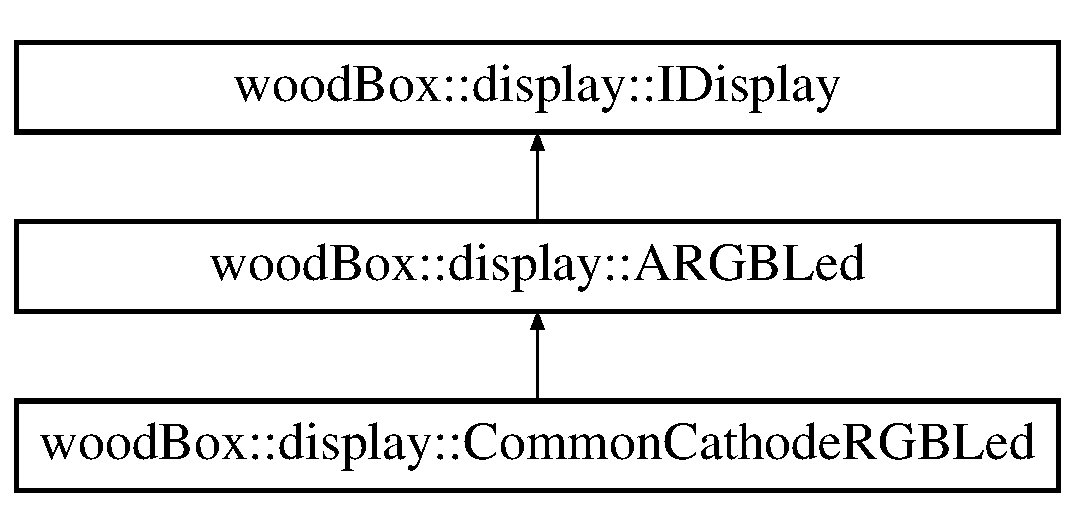
\includegraphics[height=3.000000cm]{classwood_box_1_1display_1_1_common_cathode_r_g_b_led}
\end{center}
\end{figure}
\subsection*{Public Member Functions}
\begin{DoxyCompactItemize}
\item 
\mbox{\Hypertarget{classwood_box_1_1display_1_1_common_cathode_r_g_b_led_ae80f49d3de90e4fa71c1a7b1d53c4860}\label{classwood_box_1_1display_1_1_common_cathode_r_g_b_led_ae80f49d3de90e4fa71c1a7b1d53c4860}} 
{\bfseries Common\+Cathode\+R\+G\+B\+Led} (uint8\+\_\+t, uint8\+\_\+t, uint8\+\_\+t)
\item 
\mbox{\Hypertarget{classwood_box_1_1display_1_1_common_cathode_r_g_b_led_ac51ed1f3b287d14ee7cb1bebd52dde9a}\label{classwood_box_1_1display_1_1_common_cathode_r_g_b_led_ac51ed1f3b287d14ee7cb1bebd52dde9a}} 
{\bfseries Common\+Cathode\+R\+G\+B\+Led} (const \mbox{\hyperlink{classwood_box_1_1display_1_1_common_cathode_r_g_b_led}{Common\+Cathode\+R\+G\+B\+Led}} \&)=delete
\item 
\mbox{\Hypertarget{classwood_box_1_1display_1_1_common_cathode_r_g_b_led_ac63439ba3808fb22cbcee7fb1c061b03}\label{classwood_box_1_1display_1_1_common_cathode_r_g_b_led_ac63439ba3808fb22cbcee7fb1c061b03}} 
\mbox{\hyperlink{classwood_box_1_1display_1_1_common_cathode_r_g_b_led}{Common\+Cathode\+R\+G\+B\+Led}} \& {\bfseries operator=} (const \mbox{\hyperlink{classwood_box_1_1display_1_1_common_cathode_r_g_b_led}{Common\+Cathode\+R\+G\+B\+Led}} \&)
\item 
void \mbox{\hyperlink{classwood_box_1_1display_1_1_common_cathode_r_g_b_led_a4ae3f4b7e03751dd6352adfa1b90fca0}{clear}} ()
\item 
void \mbox{\hyperlink{classwood_box_1_1display_1_1_common_cathode_r_g_b_led_a597c7ae002c7f94431ccaafd160a857a}{update}} ()
\end{DoxyCompactItemize}


\subsection{Member Function Documentation}
\mbox{\Hypertarget{classwood_box_1_1display_1_1_common_cathode_r_g_b_led_a4ae3f4b7e03751dd6352adfa1b90fca0}\label{classwood_box_1_1display_1_1_common_cathode_r_g_b_led_a4ae3f4b7e03751dd6352adfa1b90fca0}} 
\index{wood\+Box\+::display\+::\+Common\+Cathode\+R\+G\+B\+Led@{wood\+Box\+::display\+::\+Common\+Cathode\+R\+G\+B\+Led}!clear@{clear}}
\index{clear@{clear}!wood\+Box\+::display\+::\+Common\+Cathode\+R\+G\+B\+Led@{wood\+Box\+::display\+::\+Common\+Cathode\+R\+G\+B\+Led}}
\subsubsection{\texorpdfstring{clear()}{clear()}}
{\footnotesize\ttfamily void wood\+Box\+::display\+::\+Common\+Cathode\+R\+G\+B\+Led\+::clear (\begin{DoxyParamCaption}{ }\end{DoxyParamCaption})\hspace{0.3cm}{\ttfamily [virtual]}}

Remove display content 

Implements \mbox{\hyperlink{classwood_box_1_1display_1_1_a_r_g_b_led_a01eeaee1bbb439e81f5f9bc536c04df7}{wood\+Box\+::display\+::\+A\+R\+G\+B\+Led}}.

\mbox{\Hypertarget{classwood_box_1_1display_1_1_common_cathode_r_g_b_led_a597c7ae002c7f94431ccaafd160a857a}\label{classwood_box_1_1display_1_1_common_cathode_r_g_b_led_a597c7ae002c7f94431ccaafd160a857a}} 
\index{wood\+Box\+::display\+::\+Common\+Cathode\+R\+G\+B\+Led@{wood\+Box\+::display\+::\+Common\+Cathode\+R\+G\+B\+Led}!update@{update}}
\index{update@{update}!wood\+Box\+::display\+::\+Common\+Cathode\+R\+G\+B\+Led@{wood\+Box\+::display\+::\+Common\+Cathode\+R\+G\+B\+Led}}
\subsubsection{\texorpdfstring{update()}{update()}}
{\footnotesize\ttfamily void wood\+Box\+::display\+::\+Common\+Cathode\+R\+G\+B\+Led\+::update (\begin{DoxyParamCaption}{ }\end{DoxyParamCaption})\hspace{0.3cm}{\ttfamily [virtual]}}

Update display content 

Implements \mbox{\hyperlink{classwood_box_1_1display_1_1_a_r_g_b_led_ab71f321d91e931f95b96d1f492a9454d}{wood\+Box\+::display\+::\+A\+R\+G\+B\+Led}}.



The documentation for this class was generated from the following files\+:\begin{DoxyCompactItemize}
\item 
Common\+Cathode\+R\+G\+B\+Led.\+hpp\item 
Common\+Cathode\+R\+G\+B\+Led.\+cpp\end{DoxyCompactItemize}

\hypertarget{classwood_box_1_1communication_1_1wifi_1_1_e_s_p8266_wi_fi_communicator}{}\section{wood\+Box\+:\+:communication\+:\+:wifi\+:\+:E\+S\+P8266\+Wi\+Fi\+Communicator Class Reference}
\label{classwood_box_1_1communication_1_1wifi_1_1_e_s_p8266_wi_fi_communicator}\index{wood\+Box\+::communication\+::wifi\+::\+E\+S\+P8266\+Wi\+Fi\+Communicator@{wood\+Box\+::communication\+::wifi\+::\+E\+S\+P8266\+Wi\+Fi\+Communicator}}
Inheritance diagram for wood\+Box\+:\+:communication\+:\+:wifi\+:\+:E\+S\+P8266\+Wi\+Fi\+Communicator\+:\begin{figure}[H]
\begin{center}
\leavevmode
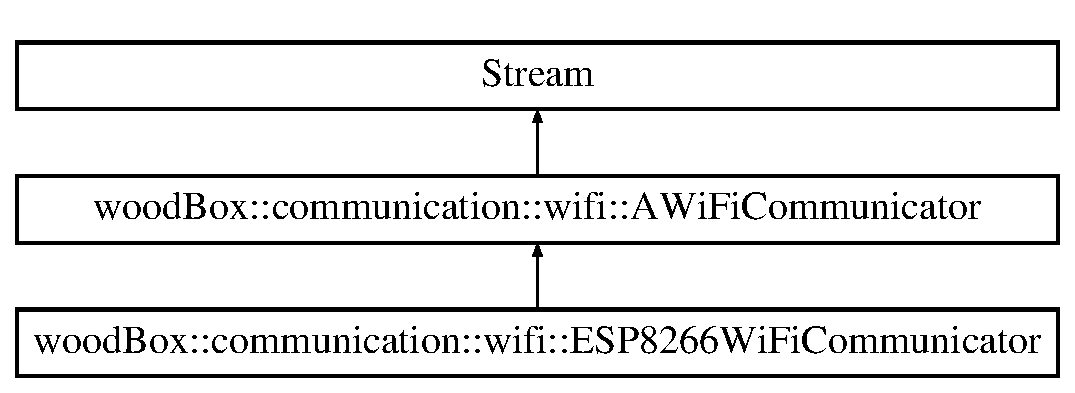
\includegraphics[height=3.000000cm]{classwood_box_1_1communication_1_1wifi_1_1_e_s_p8266_wi_fi_communicator}
\end{center}
\end{figure}
\subsection*{Public Member Functions}
\begin{DoxyCompactItemize}
\item 
\mbox{\Hypertarget{classwood_box_1_1communication_1_1wifi_1_1_e_s_p8266_wi_fi_communicator_a0af11f50c19c8d00112e61e7919294ef}\label{classwood_box_1_1communication_1_1wifi_1_1_e_s_p8266_wi_fi_communicator_a0af11f50c19c8d00112e61e7919294ef}} 
{\bfseries E\+S\+P8266\+Wi\+Fi\+Communicator} (int, int)
\item 
\mbox{\Hypertarget{classwood_box_1_1communication_1_1wifi_1_1_e_s_p8266_wi_fi_communicator_a7e7137815f9b6d8dc18adcef1ccb13cc}\label{classwood_box_1_1communication_1_1wifi_1_1_e_s_p8266_wi_fi_communicator_a7e7137815f9b6d8dc18adcef1ccb13cc}} 
{\bfseries E\+S\+P8266\+Wi\+Fi\+Communicator} (const \mbox{\hyperlink{classwood_box_1_1communication_1_1wifi_1_1_e_s_p8266_wi_fi_communicator}{E\+S\+P8266\+Wi\+Fi\+Communicator}} \&)=delete
\item 
\mbox{\Hypertarget{classwood_box_1_1communication_1_1wifi_1_1_e_s_p8266_wi_fi_communicator_a422e4ef0462beca6e66a5909b41966ef}\label{classwood_box_1_1communication_1_1wifi_1_1_e_s_p8266_wi_fi_communicator_a422e4ef0462beca6e66a5909b41966ef}} 
\mbox{\hyperlink{classwood_box_1_1communication_1_1wifi_1_1_e_s_p8266_wi_fi_communicator}{E\+S\+P8266\+Wi\+Fi\+Communicator}} \& {\bfseries operator=} (const \mbox{\hyperlink{classwood_box_1_1communication_1_1wifi_1_1_e_s_p8266_wi_fi_communicator}{E\+S\+P8266\+Wi\+Fi\+Communicator}} \&)=delete
\item 
\mbox{\Hypertarget{classwood_box_1_1communication_1_1wifi_1_1_e_s_p8266_wi_fi_communicator_aa73f46aaaf5441b79dd4a15be293aeb4}\label{classwood_box_1_1communication_1_1wifi_1_1_e_s_p8266_wi_fi_communicator_aa73f46aaaf5441b79dd4a15be293aeb4}} 
virtual int {\bfseries available} ()
\item 
\mbox{\Hypertarget{classwood_box_1_1communication_1_1wifi_1_1_e_s_p8266_wi_fi_communicator_a3bd1c8f72256e92c6dbdab9272fd3543}\label{classwood_box_1_1communication_1_1wifi_1_1_e_s_p8266_wi_fi_communicator_a3bd1c8f72256e92c6dbdab9272fd3543}} 
virtual int {\bfseries read} ()
\item 
\mbox{\Hypertarget{classwood_box_1_1communication_1_1wifi_1_1_e_s_p8266_wi_fi_communicator_accc6832fa7351cb977b9e3a805dc8107}\label{classwood_box_1_1communication_1_1wifi_1_1_e_s_p8266_wi_fi_communicator_accc6832fa7351cb977b9e3a805dc8107}} 
virtual int {\bfseries peek} ()
\item 
\mbox{\Hypertarget{classwood_box_1_1communication_1_1wifi_1_1_e_s_p8266_wi_fi_communicator_a6bb904e5302da7ec3fefc6e9a896f5f8}\label{classwood_box_1_1communication_1_1wifi_1_1_e_s_p8266_wi_fi_communicator_a6bb904e5302da7ec3fefc6e9a896f5f8}} 
virtual size\+\_\+t {\bfseries write} (uint8\+\_\+t)
\item 
\mbox{\Hypertarget{classwood_box_1_1communication_1_1wifi_1_1_e_s_p8266_wi_fi_communicator_a523aec958ef48fa917621a560d964f40}\label{classwood_box_1_1communication_1_1wifi_1_1_e_s_p8266_wi_fi_communicator_a523aec958ef48fa917621a560d964f40}} 
virtual void {\bfseries flush} ()
\item 
\mbox{\Hypertarget{classwood_box_1_1communication_1_1wifi_1_1_e_s_p8266_wi_fi_communicator_a8bf593dd2b78572988c240b57cc9c5c8}\label{classwood_box_1_1communication_1_1wifi_1_1_e_s_p8266_wi_fi_communicator_a8bf593dd2b78572988c240b57cc9c5c8}} 
void {\bfseries open} ()
\item 
\mbox{\Hypertarget{classwood_box_1_1communication_1_1wifi_1_1_e_s_p8266_wi_fi_communicator_ae8188b06891b3fd0e21312b3e69910d4}\label{classwood_box_1_1communication_1_1wifi_1_1_e_s_p8266_wi_fi_communicator_ae8188b06891b3fd0e21312b3e69910d4}} 
void {\bfseries close} ()
\item 
\mbox{\Hypertarget{classwood_box_1_1communication_1_1wifi_1_1_e_s_p8266_wi_fi_communicator_ab3e1f12a851dc3ed6eb487c39178cb6f}\label{classwood_box_1_1communication_1_1wifi_1_1_e_s_p8266_wi_fi_communicator_ab3e1f12a851dc3ed6eb487c39178cb6f}} 
virtual int {\bfseries connect} ()
\item 
\mbox{\Hypertarget{classwood_box_1_1communication_1_1wifi_1_1_e_s_p8266_wi_fi_communicator_af30a81a7f279c11241b3df0878289af0}\label{classwood_box_1_1communication_1_1wifi_1_1_e_s_p8266_wi_fi_communicator_af30a81a7f279c11241b3df0878289af0}} 
virtual int {\bfseries disconnect} ()
\item 
\mbox{\Hypertarget{classwood_box_1_1communication_1_1wifi_1_1_e_s_p8266_wi_fi_communicator_a0875cf7209c48069d22270eaeb2cac0f}\label{classwood_box_1_1communication_1_1wifi_1_1_e_s_p8266_wi_fi_communicator_a0875cf7209c48069d22270eaeb2cac0f}} 
virtual int {\bfseries connect\+To\+Host} ()
\item 
\mbox{\Hypertarget{classwood_box_1_1communication_1_1wifi_1_1_e_s_p8266_wi_fi_communicator_a5a407734df1ae47ac32575fa6346cfd4}\label{classwood_box_1_1communication_1_1wifi_1_1_e_s_p8266_wi_fi_communicator_a5a407734df1ae47ac32575fa6346cfd4}} 
virtual int {\bfseries disconnect\+From\+Host} ()
\item 
\mbox{\Hypertarget{classwood_box_1_1communication_1_1wifi_1_1_e_s_p8266_wi_fi_communicator_a66b7f8adaae85dbf94062b1cd472d98a}\label{classwood_box_1_1communication_1_1wifi_1_1_e_s_p8266_wi_fi_communicator_a66b7f8adaae85dbf94062b1cd472d98a}} 
virtual bool {\bfseries is\+Connected} ()
\end{DoxyCompactItemize}
\subsection*{Additional Inherited Members}


The documentation for this class was generated from the following files\+:\begin{DoxyCompactItemize}
\item 
E\+S\+P8266\+Wi\+Fi\+Communicator.\+hpp\item 
E\+S\+P8266\+Wi\+Fi\+Communicator.\+cpp\end{DoxyCompactItemize}

\hypertarget{classwood_box_1_1sensor_1_1_grove_air_quality_sensor}{}\section{wood\+Box\+:\+:sensor\+:\+:Grove\+Air\+Quality\+Sensor Class Reference}
\label{classwood_box_1_1sensor_1_1_grove_air_quality_sensor}\index{wood\+Box\+::sensor\+::\+Grove\+Air\+Quality\+Sensor@{wood\+Box\+::sensor\+::\+Grove\+Air\+Quality\+Sensor}}
Inheritance diagram for wood\+Box\+:\+:sensor\+:\+:Grove\+Air\+Quality\+Sensor\+:\begin{figure}[H]
\begin{center}
\leavevmode
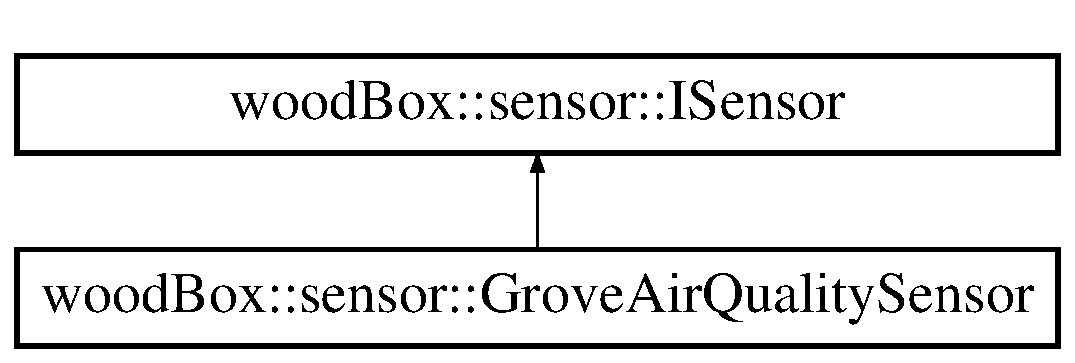
\includegraphics[height=2.000000cm]{classwood_box_1_1sensor_1_1_grove_air_quality_sensor}
\end{center}
\end{figure}
\subsection*{Public Member Functions}
\begin{DoxyCompactItemize}
\item 
\mbox{\Hypertarget{classwood_box_1_1sensor_1_1_grove_air_quality_sensor_a76692aa26d0f1debc9314faf97f3622e}\label{classwood_box_1_1sensor_1_1_grove_air_quality_sensor_a76692aa26d0f1debc9314faf97f3622e}} 
{\bfseries Grove\+Air\+Quality\+Sensor} (uint8\+\_\+t)
\item 
\mbox{\Hypertarget{classwood_box_1_1sensor_1_1_grove_air_quality_sensor_a06fcdbf2e5709b1a7936169b72c5963d}\label{classwood_box_1_1sensor_1_1_grove_air_quality_sensor_a06fcdbf2e5709b1a7936169b72c5963d}} 
{\bfseries Grove\+Air\+Quality\+Sensor} (const \mbox{\hyperlink{classwood_box_1_1sensor_1_1_grove_air_quality_sensor}{Grove\+Air\+Quality\+Sensor}} \&)=delete
\item 
\mbox{\Hypertarget{classwood_box_1_1sensor_1_1_grove_air_quality_sensor_a27e012b8973e48a28276957656fc444c}\label{classwood_box_1_1sensor_1_1_grove_air_quality_sensor_a27e012b8973e48a28276957656fc444c}} 
\mbox{\hyperlink{classwood_box_1_1sensor_1_1_grove_air_quality_sensor}{Grove\+Air\+Quality\+Sensor}} \& {\bfseries operator=} (\mbox{\hyperlink{classwood_box_1_1sensor_1_1_grove_air_quality_sensor}{Grove\+Air\+Quality\+Sensor}} \&)=delete
\item 
uint8\+\_\+t $\ast$ \mbox{\hyperlink{classwood_box_1_1sensor_1_1_grove_air_quality_sensor_a204d677110c9fe3c6b495bf9112e9afd}{get\+Sample}} ()
\item 
\mbox{\hyperlink{classwood_box_1_1sensor_1_1_i_sensor_aa377bda61ed0d4a1d7e1a7bffe459452}{I\+Sensor\+::\+I\+Sensor\+Scale}} \mbox{\hyperlink{classwood_box_1_1sensor_1_1_grove_air_quality_sensor_a457e99f530b79f14db1de00cba3e81ff}{get\+Estimate}} ()
\end{DoxyCompactItemize}
\subsection*{Additional Inherited Members}


\subsection{Member Function Documentation}
\mbox{\Hypertarget{classwood_box_1_1sensor_1_1_grove_air_quality_sensor_a457e99f530b79f14db1de00cba3e81ff}\label{classwood_box_1_1sensor_1_1_grove_air_quality_sensor_a457e99f530b79f14db1de00cba3e81ff}} 
\index{wood\+Box\+::sensor\+::\+Grove\+Air\+Quality\+Sensor@{wood\+Box\+::sensor\+::\+Grove\+Air\+Quality\+Sensor}!get\+Estimate@{get\+Estimate}}
\index{get\+Estimate@{get\+Estimate}!wood\+Box\+::sensor\+::\+Grove\+Air\+Quality\+Sensor@{wood\+Box\+::sensor\+::\+Grove\+Air\+Quality\+Sensor}}
\subsubsection{\texorpdfstring{get\+Estimate()}{getEstimate()}}
{\footnotesize\ttfamily \mbox{\hyperlink{classwood_box_1_1sensor_1_1_i_sensor_aa377bda61ed0d4a1d7e1a7bffe459452}{I\+Sensor\+::\+I\+Sensor\+Scale}} wood\+Box\+::sensor\+::\+Grove\+Air\+Quality\+Sensor\+::get\+Estimate (\begin{DoxyParamCaption}{ }\end{DoxyParamCaption})\hspace{0.3cm}{\ttfamily [virtual]}}

Returns the estimation of safety from the current sensor value

Example\+:


\begin{DoxyCode}
\textcolor{keywordtype}{void} my\_function\_telling\_if\_a\_sensor\_value\_is\_good\_or\_not(ISensor &my\_sensor) \{
  \mbox{\hyperlink{classwood_box_1_1sensor_1_1_i_sensor_aa377bda61ed0d4a1d7e1a7bffe459452}{ISensorScale}} sensor\_estimate = my\_sensor.getEstimate();
  \textcolor{keywordflow}{if} (sensor\_estimate == ISensor::ZERO) \{
    Serial.println(\textcolor{stringliteral}{"The sensor returned an invalid value"});
  \}
  \textcolor{keywordflow}{else} \textcolor{keywordflow}{if} (sensor\_estimate > ISensor::ZERO && sensor\_estimate < 6) \{
    Serial.println(\textcolor{stringliteral}{"Boouh, it's not good :("});
  \}
  \textcolor{keywordflow}{else} \{
    Serial.println(\textcolor{stringliteral}{"Yaaaay!"});
  \}
\}
\end{DoxyCode}
 

Implements \mbox{\hyperlink{classwood_box_1_1sensor_1_1_i_sensor_afb01c2473efc4a823bf5dada0048d2bc}{wood\+Box\+::sensor\+::\+I\+Sensor}}.

\mbox{\Hypertarget{classwood_box_1_1sensor_1_1_grove_air_quality_sensor_a204d677110c9fe3c6b495bf9112e9afd}\label{classwood_box_1_1sensor_1_1_grove_air_quality_sensor_a204d677110c9fe3c6b495bf9112e9afd}} 
\index{wood\+Box\+::sensor\+::\+Grove\+Air\+Quality\+Sensor@{wood\+Box\+::sensor\+::\+Grove\+Air\+Quality\+Sensor}!get\+Sample@{get\+Sample}}
\index{get\+Sample@{get\+Sample}!wood\+Box\+::sensor\+::\+Grove\+Air\+Quality\+Sensor@{wood\+Box\+::sensor\+::\+Grove\+Air\+Quality\+Sensor}}
\subsubsection{\texorpdfstring{get\+Sample()}{getSample()}}
{\footnotesize\ttfamily uint8\+\_\+t $\ast$ wood\+Box\+::sensor\+::\+Grove\+Air\+Quality\+Sensor\+::get\+Sample (\begin{DoxyParamCaption}{ }\end{DoxyParamCaption})\hspace{0.3cm}{\ttfamily [virtual]}}

Returns a pointer on sensor sample raw memory, as an array of bytes 

Implements \mbox{\hyperlink{classwood_box_1_1sensor_1_1_i_sensor_a9de8041b991b76cc2f6fcc3b6a1bf363}{wood\+Box\+::sensor\+::\+I\+Sensor}}.



The documentation for this class was generated from the following files\+:\begin{DoxyCompactItemize}
\item 
Grove\+Air\+Quality\+Sensor.\+hpp\item 
Grove\+Air\+Quality\+Sensor.\+cpp\end{DoxyCompactItemize}

\hypertarget{classwood_box_1_1display_1_1_grove_chainable_l_e_d}{}\section{wood\+Box\+:\+:display\+:\+:Grove\+Chainable\+L\+ED Class Reference}
\label{classwood_box_1_1display_1_1_grove_chainable_l_e_d}\index{wood\+Box\+::display\+::\+Grove\+Chainable\+L\+ED@{wood\+Box\+::display\+::\+Grove\+Chainable\+L\+ED}}
Inheritance diagram for wood\+Box\+:\+:display\+:\+:Grove\+Chainable\+L\+ED\+:\begin{figure}[H]
\begin{center}
\leavevmode
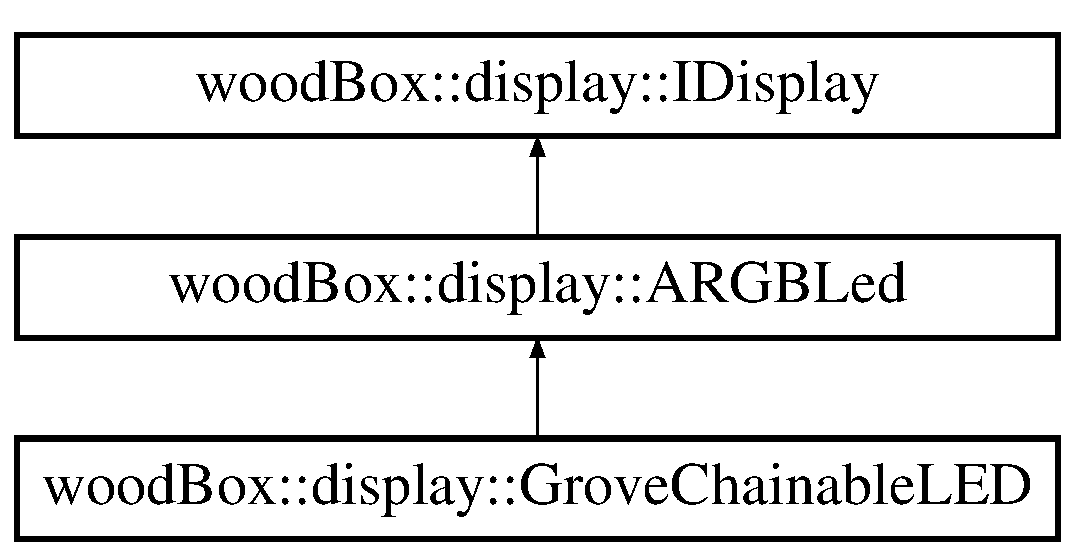
\includegraphics[height=3.000000cm]{classwood_box_1_1display_1_1_grove_chainable_l_e_d}
\end{center}
\end{figure}
\subsection*{Classes}
\begin{DoxyCompactItemize}
\item 
struct \mbox{\hyperlink{structwood_box_1_1display_1_1_grove_chainable_l_e_d_1_1_pins}{Pins}}
\end{DoxyCompactItemize}
\subsection*{Public Member Functions}
\begin{DoxyCompactItemize}
\item 
\mbox{\Hypertarget{classwood_box_1_1display_1_1_grove_chainable_l_e_d_a08c28797b0d3710c34639feb2daa5879}\label{classwood_box_1_1display_1_1_grove_chainable_l_e_d_a08c28797b0d3710c34639feb2daa5879}} 
{\bfseries Grove\+Chainable\+L\+ED} (const \mbox{\hyperlink{structwood_box_1_1display_1_1_grove_chainable_l_e_d_1_1_pins}{Pins}} $\ast$=nullptr)
\item 
\mbox{\Hypertarget{classwood_box_1_1display_1_1_grove_chainable_l_e_d_a12ecc3ce0f2316255f3d84f9ab940192}\label{classwood_box_1_1display_1_1_grove_chainable_l_e_d_a12ecc3ce0f2316255f3d84f9ab940192}} 
{\bfseries Grove\+Chainable\+L\+ED} (const \mbox{\hyperlink{structwood_box_1_1display_1_1_a_r_g_b_led_1_1_color}{A\+R\+G\+B\+Led\+::\+Color}} \&, const \mbox{\hyperlink{structwood_box_1_1display_1_1_grove_chainable_l_e_d_1_1_pins}{Pins}} $\ast$=nullptr)
\item 
\mbox{\Hypertarget{classwood_box_1_1display_1_1_grove_chainable_l_e_d_adbcc3b0c30f0f13c29d0020c053cb51b}\label{classwood_box_1_1display_1_1_grove_chainable_l_e_d_adbcc3b0c30f0f13c29d0020c053cb51b}} 
{\bfseries Grove\+Chainable\+L\+ED} (const \mbox{\hyperlink{classwood_box_1_1display_1_1_a_r_g_b_led}{A\+R\+G\+B\+Led}} \&, const \mbox{\hyperlink{structwood_box_1_1display_1_1_grove_chainable_l_e_d_1_1_pins}{Pins}} $\ast$=nullptr)
\item 
\mbox{\Hypertarget{classwood_box_1_1display_1_1_grove_chainable_l_e_d_a626699a65f024fb43a9e017bc75eae78}\label{classwood_box_1_1display_1_1_grove_chainable_l_e_d_a626699a65f024fb43a9e017bc75eae78}} 
\mbox{\hyperlink{classwood_box_1_1display_1_1_grove_chainable_l_e_d}{Grove\+Chainable\+L\+ED}} \& {\bfseries operator=} (const \mbox{\hyperlink{classwood_box_1_1display_1_1_a_r_g_b_led}{A\+R\+G\+B\+Led}} \&)
\item 
\mbox{\Hypertarget{classwood_box_1_1display_1_1_grove_chainable_l_e_d_adeb75f0b0d38e8aa842ec75b5944dc6f}\label{classwood_box_1_1display_1_1_grove_chainable_l_e_d_adeb75f0b0d38e8aa842ec75b5944dc6f}} 
\mbox{\hyperlink{classwood_box_1_1display_1_1_grove_chainable_l_e_d}{Grove\+Chainable\+L\+ED}} \& {\bfseries operator=} (const \mbox{\hyperlink{structwood_box_1_1display_1_1_a_r_g_b_led_1_1_color}{A\+R\+G\+B\+Led\+::\+Color}} \&)
\item 
virtual void \mbox{\hyperlink{classwood_box_1_1display_1_1_grove_chainable_l_e_d_a1c42c42ee9643aa914ab20a191e4adfd}{clear}} ()
\item 
virtual void \mbox{\hyperlink{classwood_box_1_1display_1_1_grove_chainable_l_e_d_a650969665d0b5607465a63159c62e4ef}{update}} ()
\end{DoxyCompactItemize}
\subsection*{Protected Attributes}
\begin{DoxyCompactItemize}
\item 
\mbox{\Hypertarget{classwood_box_1_1display_1_1_grove_chainable_l_e_d_a09907b1216ee2727c33e1c0a6e960b03}\label{classwood_box_1_1display_1_1_grove_chainable_l_e_d_a09907b1216ee2727c33e1c0a6e960b03}} 
Chainable\+L\+ED $\ast$ {\bfseries \+\_\+led}
\end{DoxyCompactItemize}


\subsection{Member Function Documentation}
\mbox{\Hypertarget{classwood_box_1_1display_1_1_grove_chainable_l_e_d_a1c42c42ee9643aa914ab20a191e4adfd}\label{classwood_box_1_1display_1_1_grove_chainable_l_e_d_a1c42c42ee9643aa914ab20a191e4adfd}} 
\index{wood\+Box\+::display\+::\+Grove\+Chainable\+L\+ED@{wood\+Box\+::display\+::\+Grove\+Chainable\+L\+ED}!clear@{clear}}
\index{clear@{clear}!wood\+Box\+::display\+::\+Grove\+Chainable\+L\+ED@{wood\+Box\+::display\+::\+Grove\+Chainable\+L\+ED}}
\subsubsection{\texorpdfstring{clear()}{clear()}}
{\footnotesize\ttfamily void wood\+Box\+::display\+::\+Grove\+Chainable\+L\+E\+D\+::clear (\begin{DoxyParamCaption}{ }\end{DoxyParamCaption})\hspace{0.3cm}{\ttfamily [virtual]}}

Remove display content 

Implements \mbox{\hyperlink{classwood_box_1_1display_1_1_a_r_g_b_led_a01eeaee1bbb439e81f5f9bc536c04df7}{wood\+Box\+::display\+::\+A\+R\+G\+B\+Led}}.

\mbox{\Hypertarget{classwood_box_1_1display_1_1_grove_chainable_l_e_d_a650969665d0b5607465a63159c62e4ef}\label{classwood_box_1_1display_1_1_grove_chainable_l_e_d_a650969665d0b5607465a63159c62e4ef}} 
\index{wood\+Box\+::display\+::\+Grove\+Chainable\+L\+ED@{wood\+Box\+::display\+::\+Grove\+Chainable\+L\+ED}!update@{update}}
\index{update@{update}!wood\+Box\+::display\+::\+Grove\+Chainable\+L\+ED@{wood\+Box\+::display\+::\+Grove\+Chainable\+L\+ED}}
\subsubsection{\texorpdfstring{update()}{update()}}
{\footnotesize\ttfamily void wood\+Box\+::display\+::\+Grove\+Chainable\+L\+E\+D\+::update (\begin{DoxyParamCaption}{ }\end{DoxyParamCaption})\hspace{0.3cm}{\ttfamily [virtual]}}

Update display content 

Implements \mbox{\hyperlink{classwood_box_1_1display_1_1_a_r_g_b_led_ab71f321d91e931f95b96d1f492a9454d}{wood\+Box\+::display\+::\+A\+R\+G\+B\+Led}}.



The documentation for this class was generated from the following files\+:\begin{DoxyCompactItemize}
\item 
Grove\+Chainable\+L\+E\+D.\+hpp\item 
Grove\+Chainable\+L\+E\+D.\+cpp\end{DoxyCompactItemize}

\hypertarget{classwood_box_1_1display_1_1_i_display}{}\section{wood\+Box\+:\+:display\+:\+:I\+Display Class Reference}
\label{classwood_box_1_1display_1_1_i_display}\index{wood\+Box\+::display\+::\+I\+Display@{wood\+Box\+::display\+::\+I\+Display}}
Inheritance diagram for wood\+Box\+:\+:display\+:\+:I\+Display\+:\begin{figure}[H]
\begin{center}
\leavevmode
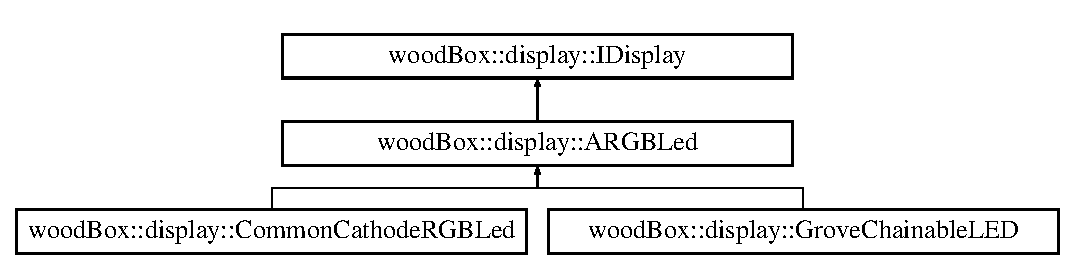
\includegraphics[height=2.000000cm]{classwood_box_1_1display_1_1_i_display}
\end{center}
\end{figure}
\subsection*{Public Member Functions}
\begin{DoxyCompactItemize}
\item 
\mbox{\Hypertarget{classwood_box_1_1display_1_1_i_display_a7030f0768c1ef15ce936a259406168dc}\label{classwood_box_1_1display_1_1_i_display_a7030f0768c1ef15ce936a259406168dc}} 
virtual void {\bfseries clear} ()=0
\item 
\mbox{\Hypertarget{classwood_box_1_1display_1_1_i_display_ad8c0811b8b807ce119a06c7806004de7}\label{classwood_box_1_1display_1_1_i_display_ad8c0811b8b807ce119a06c7806004de7}} 
virtual void {\bfseries update} ()=0
\end{DoxyCompactItemize}


The documentation for this class was generated from the following file\+:\begin{DoxyCompactItemize}
\item 
I\+Display.\+hpp\end{DoxyCompactItemize}

\hypertarget{classwood_box_1_1power_1_1_i_power}{}\section{wood\+Box\+:\+:power\+:\+:I\+Power Class Reference}
\label{classwood_box_1_1power_1_1_i_power}\index{wood\+Box\+::power\+::\+I\+Power@{wood\+Box\+::power\+::\+I\+Power}}
\subsection*{Public Member Functions}
\begin{DoxyCompactItemize}
\item 
\mbox{\Hypertarget{classwood_box_1_1power_1_1_i_power_a4645f7d9dbbaee583ba2446ef35a8635}\label{classwood_box_1_1power_1_1_i_power_a4645f7d9dbbaee583ba2446ef35a8635}} 
virtual bool {\bfseries is\+Working} ()=0
\item 
\mbox{\Hypertarget{classwood_box_1_1power_1_1_i_power_a67086e56aca8cb46033a441b3f4e11aa}\label{classwood_box_1_1power_1_1_i_power_a67086e56aca8cb46033a441b3f4e11aa}} 
virtual uint32\+\_\+t {\bfseries get\+Voltage} ()=0
\item 
\mbox{\Hypertarget{classwood_box_1_1power_1_1_i_power_a9b3e0363c22d3064bd7ccc8663f1a033}\label{classwood_box_1_1power_1_1_i_power_a9b3e0363c22d3064bd7ccc8663f1a033}} 
virtual uint32\+\_\+t {\bfseries get\+Current} ()=0
\end{DoxyCompactItemize}


The documentation for this class was generated from the following file\+:\begin{DoxyCompactItemize}
\item 
I\+Power.\+hpp\end{DoxyCompactItemize}

\hypertarget{classwood_box_1_1sensor_1_1_i_sensor}{}\section{wood\+Box\+:\+:sensor\+:\+:I\+Sensor Class Reference}
\label{classwood_box_1_1sensor_1_1_i_sensor}\index{wood\+Box\+::sensor\+::\+I\+Sensor@{wood\+Box\+::sensor\+::\+I\+Sensor}}
Inheritance diagram for wood\+Box\+:\+:sensor\+:\+:I\+Sensor\+:\begin{figure}[H]
\begin{center}
\leavevmode
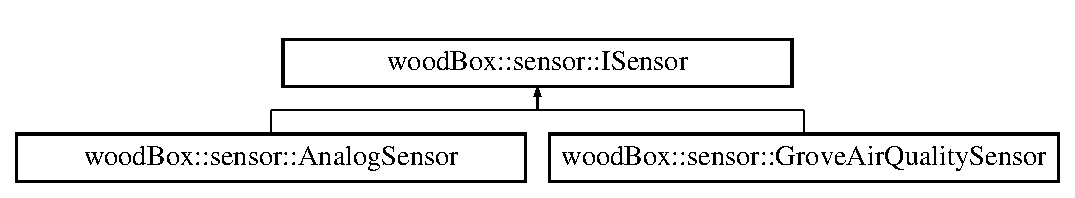
\includegraphics[height=2.000000cm]{classwood_box_1_1sensor_1_1_i_sensor}
\end{center}
\end{figure}
\subsection*{Public Member Functions}
\begin{DoxyCompactItemize}
\item 
\mbox{\Hypertarget{classwood_box_1_1sensor_1_1_i_sensor_ac772909aea9d8556cdda19841d3bbc40}\label{classwood_box_1_1sensor_1_1_i_sensor_ac772909aea9d8556cdda19841d3bbc40}} 
virtual void {\bfseries init} ()=0
\item 
\mbox{\Hypertarget{classwood_box_1_1sensor_1_1_i_sensor_a801f29792a0cd49bef0c54b346c570ad}\label{classwood_box_1_1sensor_1_1_i_sensor_a801f29792a0cd49bef0c54b346c570ad}} 
virtual void {\bfseries stop} ()=0
\item 
\mbox{\Hypertarget{classwood_box_1_1sensor_1_1_i_sensor_a9de8041b991b76cc2f6fcc3b6a1bf363}\label{classwood_box_1_1sensor_1_1_i_sensor_a9de8041b991b76cc2f6fcc3b6a1bf363}} 
virtual uint8\+\_\+t $\ast$ {\bfseries get\+Sample} ()=0
\end{DoxyCompactItemize}


The documentation for this class was generated from the following file\+:\begin{DoxyCompactItemize}
\item 
I\+Sensor.\+hpp\end{DoxyCompactItemize}

\hypertarget{classwood_box_1_1storage_1_1_i_storage}{}\section{wood\+Box\+:\+:storage\+:\+:I\+Storage Class Reference}
\label{classwood_box_1_1storage_1_1_i_storage}\index{wood\+Box\+::storage\+::\+I\+Storage@{wood\+Box\+::storage\+::\+I\+Storage}}


{\ttfamily \#include $<$I\+Storage.\+hpp$>$}

\subsection*{Public Member Functions}
\begin{DoxyCompactItemize}
\item 
virtual void \mbox{\hyperlink{classwood_box_1_1storage_1_1_i_storage_a01bab924be0844e3866b27279caa506d}{read}} (size\+\_\+t, void $\ast$, size\+\_\+t)=0
\item 
virtual void \mbox{\hyperlink{classwood_box_1_1storage_1_1_i_storage_a5eb82c922e8a3147ddab510706be8e24}{write}} (size\+\_\+t, const void $\ast$, size\+\_\+t)=0
\end{DoxyCompactItemize}


\subsection{Detailed Description}
Interface used to be able to store and read raw data from any source, by transferring memory buffers 

\subsection{Member Function Documentation}
\mbox{\Hypertarget{classwood_box_1_1storage_1_1_i_storage_a01bab924be0844e3866b27279caa506d}\label{classwood_box_1_1storage_1_1_i_storage_a01bab924be0844e3866b27279caa506d}} 
\index{wood\+Box\+::storage\+::\+I\+Storage@{wood\+Box\+::storage\+::\+I\+Storage}!read@{read}}
\index{read@{read}!wood\+Box\+::storage\+::\+I\+Storage@{wood\+Box\+::storage\+::\+I\+Storage}}
\subsubsection{\texorpdfstring{read()}{read()}}
{\footnotesize\ttfamily virtual void wood\+Box\+::storage\+::\+I\+Storage\+::read (\begin{DoxyParamCaption}\item[{size\+\_\+t}]{,  }\item[{void $\ast$}]{,  }\item[{size\+\_\+t}]{ }\end{DoxyParamCaption})\hspace{0.3cm}{\ttfamily [pure virtual]}}

Copy n bytes (3rd parameter) in dest (2nd parameter) from offset x (1st parameter) \mbox{\Hypertarget{classwood_box_1_1storage_1_1_i_storage_a5eb82c922e8a3147ddab510706be8e24}\label{classwood_box_1_1storage_1_1_i_storage_a5eb82c922e8a3147ddab510706be8e24}} 
\index{wood\+Box\+::storage\+::\+I\+Storage@{wood\+Box\+::storage\+::\+I\+Storage}!write@{write}}
\index{write@{write}!wood\+Box\+::storage\+::\+I\+Storage@{wood\+Box\+::storage\+::\+I\+Storage}}
\subsubsection{\texorpdfstring{write()}{write()}}
{\footnotesize\ttfamily virtual void wood\+Box\+::storage\+::\+I\+Storage\+::write (\begin{DoxyParamCaption}\item[{size\+\_\+t}]{,  }\item[{const void $\ast$}]{,  }\item[{size\+\_\+t}]{ }\end{DoxyParamCaption})\hspace{0.3cm}{\ttfamily [pure virtual]}}

Write n bytes (3rd parameter) in offset x (1st parameter) from src (2nd parameter) 

The documentation for this class was generated from the following file\+:\begin{DoxyCompactItemize}
\item 
I\+Storage.\+hpp\end{DoxyCompactItemize}

\hypertarget{classwood_box_1_1display_1_1_neo_pixel}{}\section{wood\+Box\+:\+:display\+:\+:Neo\+Pixel Class Reference}
\label{classwood_box_1_1display_1_1_neo_pixel}\index{wood\+Box\+::display\+::\+Neo\+Pixel@{wood\+Box\+::display\+::\+Neo\+Pixel}}
Inheritance diagram for wood\+Box\+:\+:display\+:\+:Neo\+Pixel\+:\begin{figure}[H]
\begin{center}
\leavevmode
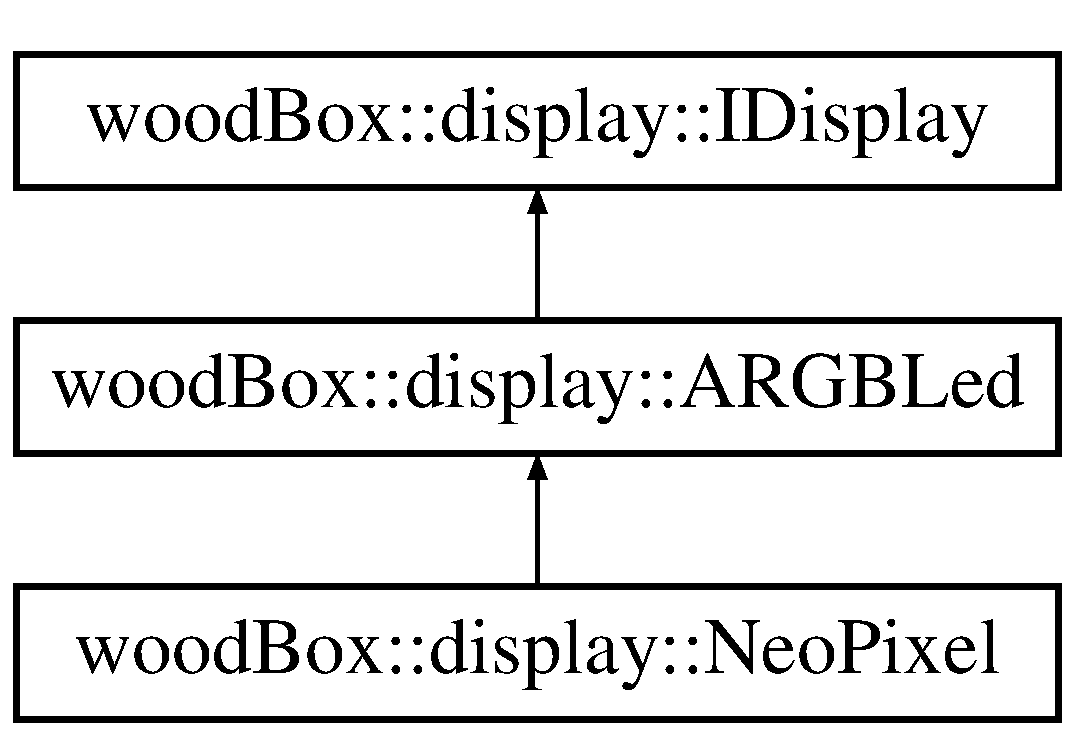
\includegraphics[height=3.000000cm]{classwood_box_1_1display_1_1_neo_pixel}
\end{center}
\end{figure}
\subsection*{Public Member Functions}
\begin{DoxyCompactItemize}
\item 
\mbox{\Hypertarget{classwood_box_1_1display_1_1_neo_pixel_a9ca8f40559e25bb7b4882bbe53764825}\label{classwood_box_1_1display_1_1_neo_pixel_a9ca8f40559e25bb7b4882bbe53764825}} 
{\bfseries Neo\+Pixel} (uint8\+\_\+t, neo\+Pixel\+Type=N\+E\+O\+\_\+\+G\+RB+N\+E\+O\+\_\+\+K\+H\+Z800)
\item 
\mbox{\Hypertarget{classwood_box_1_1display_1_1_neo_pixel_a2f2e2a778c2d365794daf4c232922035}\label{classwood_box_1_1display_1_1_neo_pixel_a2f2e2a778c2d365794daf4c232922035}} 
{\bfseries Neo\+Pixel} (const \mbox{\hyperlink{classwood_box_1_1display_1_1_neo_pixel}{Neo\+Pixel}} \&)=delete
\item 
\mbox{\Hypertarget{classwood_box_1_1display_1_1_neo_pixel_a82aa2f0f6c13db9b11126a0389e72936}\label{classwood_box_1_1display_1_1_neo_pixel_a82aa2f0f6c13db9b11126a0389e72936}} 
{\bfseries Neo\+Pixel} (uint8\+\_\+t, const \mbox{\hyperlink{classwood_box_1_1display_1_1_neo_pixel}{Neo\+Pixel}} \&)
\item 
\mbox{\Hypertarget{classwood_box_1_1display_1_1_neo_pixel_a5b187e7ce528d7da80568d627813595d}\label{classwood_box_1_1display_1_1_neo_pixel_a5b187e7ce528d7da80568d627813595d}} 
\mbox{\hyperlink{classwood_box_1_1display_1_1_neo_pixel}{Neo\+Pixel}} \& {\bfseries operator=} (const \mbox{\hyperlink{classwood_box_1_1display_1_1_neo_pixel}{Neo\+Pixel}} \&)
\item 
void \mbox{\hyperlink{classwood_box_1_1display_1_1_neo_pixel_ac2ec48825a10154e0ef99c4d8010aa6e}{update}} ()
\end{DoxyCompactItemize}


\subsection{Member Function Documentation}
\mbox{\Hypertarget{classwood_box_1_1display_1_1_neo_pixel_ac2ec48825a10154e0ef99c4d8010aa6e}\label{classwood_box_1_1display_1_1_neo_pixel_ac2ec48825a10154e0ef99c4d8010aa6e}} 
\index{wood\+Box\+::display\+::\+Neo\+Pixel@{wood\+Box\+::display\+::\+Neo\+Pixel}!update@{update}}
\index{update@{update}!wood\+Box\+::display\+::\+Neo\+Pixel@{wood\+Box\+::display\+::\+Neo\+Pixel}}
\subsubsection{\texorpdfstring{update()}{update()}}
{\footnotesize\ttfamily void wood\+Box\+::display\+::\+Neo\+Pixel\+::update (\begin{DoxyParamCaption}{ }\end{DoxyParamCaption})\hspace{0.3cm}{\ttfamily [virtual]}}

Update display content 

Implements \mbox{\hyperlink{classwood_box_1_1display_1_1_a_r_g_b_led_ab71f321d91e931f95b96d1f492a9454d}{wood\+Box\+::display\+::\+A\+R\+G\+B\+Led}}.



The documentation for this class was generated from the following files\+:\begin{DoxyCompactItemize}
\item 
Neo\+Pixel.\+hpp\item 
Neo\+Pixel.\+cpp\end{DoxyCompactItemize}

\hypertarget{structwood_box_1_1display_1_1_grove_chainable_l_e_d_1_1_pins}{}\section{wood\+Box\+:\+:display\+:\+:Grove\+Chainable\+L\+ED\+:\+:Pins Struct Reference}
\label{structwood_box_1_1display_1_1_grove_chainable_l_e_d_1_1_pins}\index{wood\+Box\+::display\+::\+Grove\+Chainable\+L\+E\+D\+::\+Pins@{wood\+Box\+::display\+::\+Grove\+Chainable\+L\+E\+D\+::\+Pins}}
\subsection*{Public Attributes}
\begin{DoxyCompactItemize}
\item 
\mbox{\Hypertarget{structwood_box_1_1display_1_1_grove_chainable_l_e_d_1_1_pins_a6cd497a670cf643e24c162c028ba437d}\label{structwood_box_1_1display_1_1_grove_chainable_l_e_d_1_1_pins_a6cd497a670cf643e24c162c028ba437d}} 
uint8\+\_\+t {\bfseries clock}
\item 
\mbox{\Hypertarget{structwood_box_1_1display_1_1_grove_chainable_l_e_d_1_1_pins_ad2d837c604afe7978b05e8fa4654e9b4}\label{structwood_box_1_1display_1_1_grove_chainable_l_e_d_1_1_pins_ad2d837c604afe7978b05e8fa4654e9b4}} 
uint8\+\_\+t {\bfseries data}
\end{DoxyCompactItemize}


The documentation for this struct was generated from the following file\+:\begin{DoxyCompactItemize}
\item 
Grove\+Chainable\+L\+E\+D.\+hpp\end{DoxyCompactItemize}

\hypertarget{classwood_box_1_1utility_1_1_queue}{}\section{wood\+Box\+:\+:utility\+:\+:Queue$<$ T $>$ Class Template Reference}
\label{classwood_box_1_1utility_1_1_queue}\index{wood\+Box\+::utility\+::\+Queue$<$ T $>$@{wood\+Box\+::utility\+::\+Queue$<$ T $>$}}
Inheritance diagram for wood\+Box\+:\+:utility\+:\+:Queue$<$ T $>$\+:\begin{figure}[H]
\begin{center}
\leavevmode
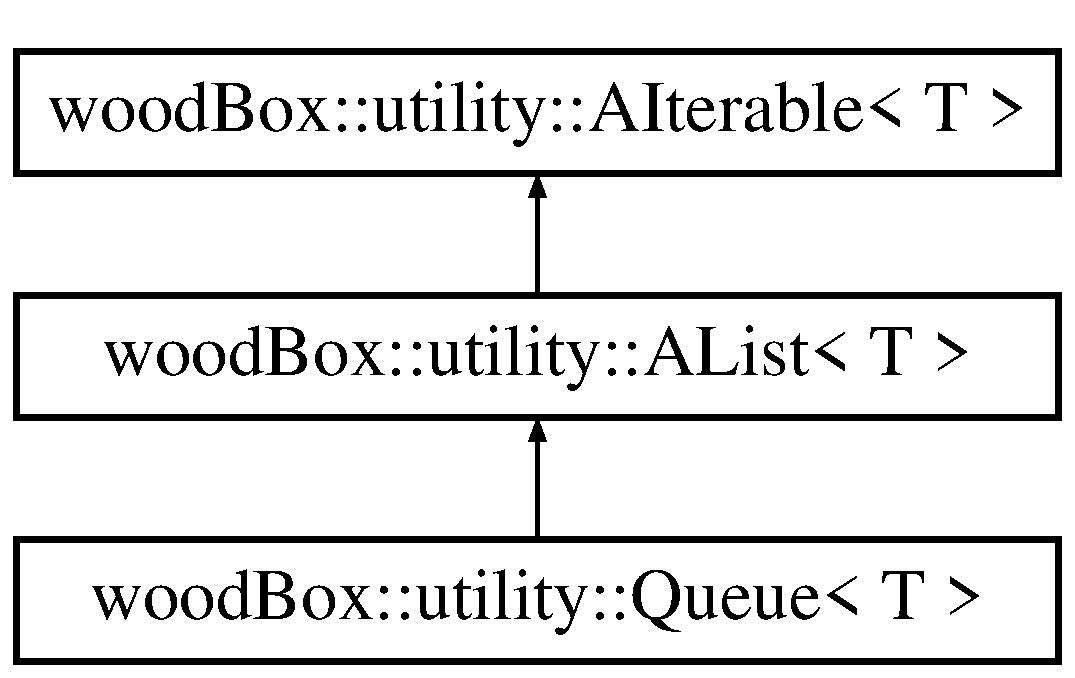
\includegraphics[height=3.000000cm]{classwood_box_1_1utility_1_1_queue}
\end{center}
\end{figure}
\subsection*{Public Member Functions}
\begin{DoxyCompactItemize}
\item 
\mbox{\Hypertarget{classwood_box_1_1utility_1_1_queue_a3fd68bd9b7d12606445926b4e26e763c}\label{classwood_box_1_1utility_1_1_queue_a3fd68bd9b7d12606445926b4e26e763c}} 
{\bfseries Queue} (T \&data)
\item 
\mbox{\Hypertarget{classwood_box_1_1utility_1_1_queue_a811d00da7a7cefd7e3551a1381396a96}\label{classwood_box_1_1utility_1_1_queue_a811d00da7a7cefd7e3551a1381396a96}} 
{\bfseries Queue} (const \mbox{\hyperlink{classwood_box_1_1utility_1_1_queue}{Queue}} \&)=delete
\item 
\mbox{\Hypertarget{classwood_box_1_1utility_1_1_queue_a2c9fea4bcd5ee866d5d81b80a4ff6c6d}\label{classwood_box_1_1utility_1_1_queue_a2c9fea4bcd5ee866d5d81b80a4ff6c6d}} 
\mbox{\hyperlink{classwood_box_1_1utility_1_1_queue}{Queue}} \& {\bfseries operator=} (const \mbox{\hyperlink{classwood_box_1_1utility_1_1_queue}{Queue}} \&)=delete
\item 
\mbox{\Hypertarget{classwood_box_1_1utility_1_1_queue_a027d2b2c9fe678f913ddaf462b37669c}\label{classwood_box_1_1utility_1_1_queue_a027d2b2c9fe678f913ddaf462b37669c}} 
\mbox{\hyperlink{classwood_box_1_1utility_1_1_queue}{Queue}} \& {\bfseries append} (T \&data)
\end{DoxyCompactItemize}
\subsection*{Additional Inherited Members}


The documentation for this class was generated from the following file\+:\begin{DoxyCompactItemize}
\item 
Queue.\+hpp\end{DoxyCompactItemize}

\hypertarget{structwood_box_1_1communication_1_1ip_1_1s__host}{}\section{wood\+Box\+:\+:communication\+:\+:ip\+:\+:s\+\_\+host Struct Reference}
\label{structwood_box_1_1communication_1_1ip_1_1s__host}\index{wood\+Box\+::communication\+::ip\+::s\+\_\+host@{wood\+Box\+::communication\+::ip\+::s\+\_\+host}}
\subsection*{Public Attributes}
\begin{DoxyCompactItemize}
\item 
\mbox{\Hypertarget{structwood_box_1_1communication_1_1ip_1_1s__host_ab867830a8b43080c199f4006067b2c22}\label{structwood_box_1_1communication_1_1ip_1_1s__host_ab867830a8b43080c199f4006067b2c22}} 
\begin{tabbing}
xx\=xx\=xx\=xx\=xx\=xx\=xx\=xx\=xx\=\kill
union \{\\
\>ipv6\_address {\bfseries ipv6}\\
\>ipv4\_address {\bfseries ipv4}\\
\}; \\

\end{tabbing}\item 
\mbox{\Hypertarget{structwood_box_1_1communication_1_1ip_1_1s__host_ae4df433233593fc00345f6372f78bd37}\label{structwood_box_1_1communication_1_1ip_1_1s__host_ae4df433233593fc00345f6372f78bd37}} 
port {\bfseries hport}
\end{DoxyCompactItemize}


The documentation for this struct was generated from the following file\+:\begin{DoxyCompactItemize}
\item 
network\+\_\+ip\+\_\+types.\+hpp\end{DoxyCompactItemize}

\hypertarget{structwood_box_1_1communication_1_1wifi_1_1s__wifi__access__point}{}\section{wood\+Box\+:\+:communication\+:\+:wifi\+:\+:s\+\_\+wifi\+\_\+access\+\_\+point Struct Reference}
\label{structwood_box_1_1communication_1_1wifi_1_1s__wifi__access__point}\index{wood\+Box\+::communication\+::wifi\+::s\+\_\+wifi\+\_\+access\+\_\+point@{wood\+Box\+::communication\+::wifi\+::s\+\_\+wifi\+\_\+access\+\_\+point}}
\subsection*{Public Attributes}
\begin{DoxyCompactItemize}
\item 
\mbox{\Hypertarget{structwood_box_1_1communication_1_1wifi_1_1s__wifi__access__point_ac5bbb7d91e2794c134b8e3f166c9d2ab}\label{structwood_box_1_1communication_1_1wifi_1_1s__wifi__access__point_ac5bbb7d91e2794c134b8e3f166c9d2ab}} 
wifi\+\_\+ssid {\bfseries ssid}
\item 
\mbox{\Hypertarget{structwood_box_1_1communication_1_1wifi_1_1s__wifi__access__point_a0a706e0c1992ea3b1ef539497a6d818e}\label{structwood_box_1_1communication_1_1wifi_1_1s__wifi__access__point_a0a706e0c1992ea3b1ef539497a6d818e}} 
wifi\+\_\+password {\bfseries password}
\item 
\mbox{\Hypertarget{structwood_box_1_1communication_1_1wifi_1_1s__wifi__access__point_a6729c2e3c331f4946a64120bc88032bc}\label{structwood_box_1_1communication_1_1wifi_1_1s__wifi__access__point_a6729c2e3c331f4946a64120bc88032bc}} 
wifi\+\_\+channel {\bfseries channel}
\item 
\mbox{\Hypertarget{structwood_box_1_1communication_1_1wifi_1_1s__wifi__access__point_a9a629ae193603ac7de1c846b7e093d7d}\label{structwood_box_1_1communication_1_1wifi_1_1s__wifi__access__point_a9a629ae193603ac7de1c846b7e093d7d}} 
wifi\+\_\+norm {\bfseries norm}
\item 
\mbox{\Hypertarget{structwood_box_1_1communication_1_1wifi_1_1s__wifi__access__point_a02c57a98f9ad2ada4a966ddd4cbc80c2}\label{structwood_box_1_1communication_1_1wifi_1_1s__wifi__access__point_a02c57a98f9ad2ada4a966ddd4cbc80c2}} 
wifi\+\_\+frequency\+\_\+band {\bfseries band}
\end{DoxyCompactItemize}


The documentation for this struct was generated from the following file\+:\begin{DoxyCompactItemize}
\item 
wifi\+\_\+types.\+hpp\end{DoxyCompactItemize}

\hypertarget{structwood_box_1_1communication_1_1wifi_1_1s__wifi__client}{}\section{wood\+Box\+:\+:communication\+:\+:wifi\+:\+:s\+\_\+wifi\+\_\+client Struct Reference}
\label{structwood_box_1_1communication_1_1wifi_1_1s__wifi__client}\index{wood\+Box\+::communication\+::wifi\+::s\+\_\+wifi\+\_\+client@{wood\+Box\+::communication\+::wifi\+::s\+\_\+wifi\+\_\+client}}
\subsection*{Public Attributes}
\begin{DoxyCompactItemize}
\item 
\mbox{\Hypertarget{structwood_box_1_1communication_1_1wifi_1_1s__wifi__client_a0c2a084f86b4588303015c0301bc8825}\label{structwood_box_1_1communication_1_1wifi_1_1s__wifi__client_a0c2a084f86b4588303015c0301bc8825}} 
ip\+::mac\+\_\+address {\bfseries mac}
\item 
\mbox{\Hypertarget{structwood_box_1_1communication_1_1wifi_1_1s__wifi__client_afe0ae3583e2155c21e14d2376581b6ed}\label{structwood_box_1_1communication_1_1wifi_1_1s__wifi__client_afe0ae3583e2155c21e14d2376581b6ed}} 
ip\+::ipv4\+\_\+address {\bfseries ipv4}
\item 
\mbox{\Hypertarget{structwood_box_1_1communication_1_1wifi_1_1s__wifi__client_a7a17a029a3d33f6d7f03ee6507d38d8d}\label{structwood_box_1_1communication_1_1wifi_1_1s__wifi__client_a7a17a029a3d33f6d7f03ee6507d38d8d}} 
ip\+::ipv6\+\_\+address {\bfseries ipv6}
\end{DoxyCompactItemize}


The documentation for this struct was generated from the following file\+:\begin{DoxyCompactItemize}
\item 
wifi\+\_\+types.\+hpp\end{DoxyCompactItemize}

\hypertarget{classwood_box_1_1module_1_1_wood_box_module}{}\section{wood\+Box\+:\+:module\+:\+:Wood\+Box\+Module$<$ T, n $>$ Class Template Reference}
\label{classwood_box_1_1module_1_1_wood_box_module}\index{wood\+Box\+::module\+::\+Wood\+Box\+Module$<$ T, n $>$@{wood\+Box\+::module\+::\+Wood\+Box\+Module$<$ T, n $>$}}


{\ttfamily \#include $<$Wood\+Box\+Module.\+hpp$>$}

Inheritance diagram for wood\+Box\+:\+:module\+:\+:Wood\+Box\+Module$<$ T, n $>$\+:\begin{figure}[H]
\begin{center}
\leavevmode
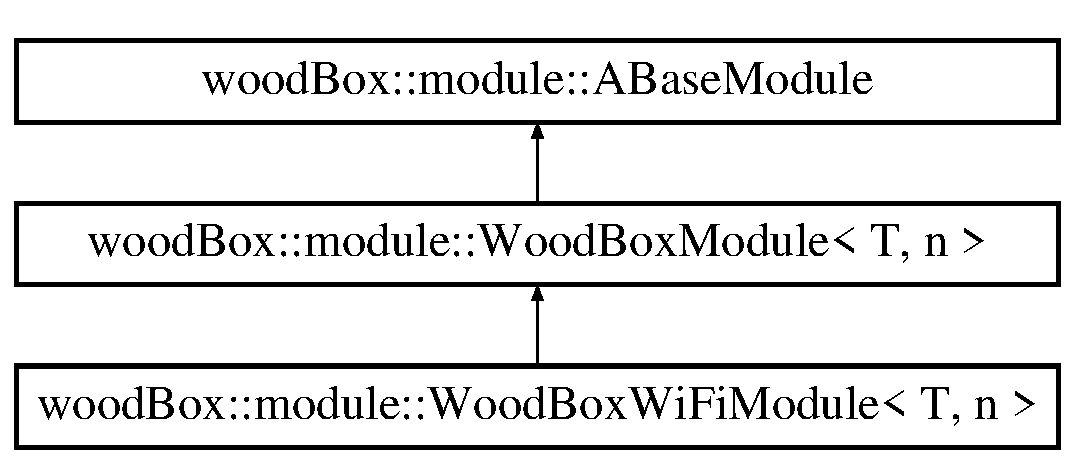
\includegraphics[height=3.000000cm]{classwood_box_1_1module_1_1_wood_box_module}
\end{center}
\end{figure}
\subsection*{Public Types}
\begin{DoxyCompactItemize}
\item 
enum \mbox{\hyperlink{classwood_box_1_1module_1_1_wood_box_module_af74476c8a785de7fe587c4fb68435673}{module\+Type}} \{ \newline
{\bfseries U\+N\+K\+N\+O\+WN}, 
{\bfseries A\+I\+R\+\_\+\+Q\+U\+A\+L\+I\+TY}, 
{\bfseries T\+E\+M\+P\+E\+R\+A\+T\+U\+RE}, 
{\bfseries H\+U\+M\+I\+D\+I\+TY}, 
\newline
{\bfseries L\+U\+M\+I\+N\+O\+S\+I\+TY}, 
{\bfseries N\+O\+I\+SE}, 
{\bfseries C\+A\+R\+B\+ON}, 
{\bfseries C\+A\+R\+B\+O\+N\+\_\+\+M\+O\+N\+O\+X\+Y\+DE}, 
\newline
{\bfseries E\+L\+E\+C\+T\+R\+O\+M\+A\+G\+N\+E\+T\+IC}, 
{\bfseries R\+A\+D\+I\+O\+A\+C\+T\+I\+V\+I\+TY}
 \}
\item 
typedef char \mbox{\hyperlink{classwood_box_1_1module_1_1_wood_box_module_adf5d59bae2980ff138284d0fa885df19}{module\+Vendor}}\mbox{[}33\mbox{]}
\item 
typedef char \mbox{\hyperlink{classwood_box_1_1module_1_1_wood_box_module_a3a6503bbd5147a06ba50081f97177b46}{module\+Serial}}\mbox{[}33\mbox{]}
\item 
typedef unsigned long \mbox{\hyperlink{classwood_box_1_1module_1_1_wood_box_module_ab03bf835ec02656605c3c0df0188dc28}{timestamp}}
\item 
typedef void($\ast$ \mbox{\hyperlink{classwood_box_1_1module_1_1_wood_box_module_ab6d400f05cc572fb9fd28dd0baf6d346}{custom\+Callback}}) ()
\item 
typedef void($\ast$ \mbox{\hyperlink{classwood_box_1_1module_1_1_wood_box_module_ab0e08bb82f5585fd357ce1881855d0e2}{Wood\+Box\+Command\+Plugin}}) (const String \&, Stream \&)
\item 
typedef void($\ast$ \mbox{\hyperlink{classwood_box_1_1module_1_1_wood_box_module_ac7fea0a06e9fcab2ffb63500f6cd6565}{Wood\+Box\+Storage\+Plugin}}) (size\+\_\+t, \mbox{\hyperlink{classwood_box_1_1storage_1_1_i_storage}{storage\+::\+I\+Storage}} \&)
\end{DoxyCompactItemize}
\subsection*{Public Member Functions}
\begin{DoxyCompactItemize}
\item 
\mbox{\hyperlink{classwood_box_1_1module_1_1_wood_box_module_ade3d82ff1e508da2ad37185c208f9333}{Wood\+Box\+Module}} (const \mbox{\hyperlink{classwood_box_1_1module_1_1_wood_box_module}{Wood\+Box\+Module}} \&)=delete
\item 
\mbox{\hyperlink{classwood_box_1_1module_1_1_wood_box_module}{Wood\+Box\+Module}} \& \mbox{\hyperlink{classwood_box_1_1module_1_1_wood_box_module_acdae18f8e9e685cdbce5a4fc99956ab3}{operator=}} (const \mbox{\hyperlink{classwood_box_1_1module_1_1_wood_box_module}{Wood\+Box\+Module}} \&)=delete
\item 
Scheduler \& \mbox{\hyperlink{classwood_box_1_1module_1_1_wood_box_module_a24b14dd95e7b1c5a7ba31107cd0c524d}{get\+Scheduler}} ()
\item 
void \mbox{\hyperlink{classwood_box_1_1module_1_1_wood_box_module_a610b2339bd0ff26d2cde59d2006a4aed}{setup}} ()
\item 
void \mbox{\hyperlink{classwood_box_1_1module_1_1_wood_box_module_ac65e58ab2338b1e3f57e4ce5d9e70c6c}{run}} ()
\item 
void \mbox{\hyperlink{classwood_box_1_1module_1_1_wood_box_module_abbc32e89fe1ace40f447539237c0b713}{stop}} ()
\item 
void \mbox{\hyperlink{classwood_box_1_1module_1_1_wood_box_module_aa5e44c8631ee30e85c16ffc0454c8210}{set\+Sensor\+Execution\+Interval}} (unsigned long ms)
\item 
void \mbox{\hyperlink{classwood_box_1_1module_1_1_wood_box_module_a0242f49765460d7c1e0528260ba1c26e}{set\+Communication\+Execution\+Interval}} (unsigned long ms)
\item 
void \mbox{\hyperlink{classwood_box_1_1module_1_1_wood_box_module_ada9e2ee4b4da9396c504c0d0217d0c2f}{set\+Upload\+Data\+Execution\+Interval}} (unsigned long ms)
\item 
unsigned long \mbox{\hyperlink{classwood_box_1_1module_1_1_wood_box_module_a4d5b8fd2ec5aeacb5704435bb6d961e7}{get\+Sensor\+Execution\+Interval}} () const
\item 
unsigned long \mbox{\hyperlink{classwood_box_1_1module_1_1_wood_box_module_ad4a7b447a617d9c6908ef624cfd2cab4}{get\+Communication\+Execution\+Interval}} () const
\item 
unsigned long \mbox{\hyperlink{classwood_box_1_1module_1_1_wood_box_module_a9582f3340d1aa35abfe278dec41f4313}{get\+Upload\+Data\+Execution\+Interval}} () const
\item 
void \mbox{\hyperlink{classwood_box_1_1module_1_1_wood_box_module_ab04481aafdcb9f3ff5ac9c9567f06006}{set\+Sensor\+Execution\+Callback}} (\mbox{\hyperlink{classwood_box_1_1module_1_1_wood_box_module_ab6d400f05cc572fb9fd28dd0baf6d346}{custom\+Callback}} f=nullptr)
\item 
void \mbox{\hyperlink{classwood_box_1_1module_1_1_wood_box_module_af75fdaa122bfa637b3c0273a699adaef}{set\+Communication\+Execution\+Callback}} (\mbox{\hyperlink{classwood_box_1_1module_1_1_wood_box_module_ab6d400f05cc572fb9fd28dd0baf6d346}{custom\+Callback}} f=nullptr)
\item 
void \mbox{\hyperlink{classwood_box_1_1module_1_1_wood_box_module_a1912f897cb51233fdfeb061211dee3d2}{set\+Upload\+Data\+Execution\+Callback}} (\mbox{\hyperlink{classwood_box_1_1module_1_1_wood_box_module_ab6d400f05cc572fb9fd28dd0baf6d346}{custom\+Callback}} f=nullptr)
\item 
void \mbox{\hyperlink{classwood_box_1_1module_1_1_wood_box_module_ad40df0835ac2ffcec83cfb96d12f9079}{set\+Command\+Plugin}} (\mbox{\hyperlink{classwood_box_1_1module_1_1_wood_box_module_ab0e08bb82f5585fd357ce1881855d0e2}{Wood\+Box\+Command\+Plugin}} plugin)
\item 
void \mbox{\hyperlink{classwood_box_1_1module_1_1_wood_box_module_a94cfcf71ecd1d715d14752001fbc7b6a}{set\+On\+Backup\+Plugin}} (\mbox{\hyperlink{classwood_box_1_1module_1_1_wood_box_module_ac7fea0a06e9fcab2ffb63500f6cd6565}{Wood\+Box\+Storage\+Plugin}} plugin)
\item 
void \mbox{\hyperlink{classwood_box_1_1module_1_1_wood_box_module_a85d4efff4708d41e3097479ab364faac}{set\+On\+Restore\+Plugin}} (\mbox{\hyperlink{classwood_box_1_1module_1_1_wood_box_module_ac7fea0a06e9fcab2ffb63500f6cd6565}{Wood\+Box\+Storage\+Plugin}} plugin)
\item 
\mbox{\hyperlink{classwood_box_1_1module_1_1_wood_box_module_af74476c8a785de7fe587c4fb68435673}{module\+Type}} \mbox{\hyperlink{classwood_box_1_1module_1_1_wood_box_module_ab2507312ea013ea5c95b8e1731ddc81d}{get\+Type}} () const
\item 
const \mbox{\hyperlink{classwood_box_1_1module_1_1_wood_box_module_adf5d59bae2980ff138284d0fa885df19}{module\+Vendor}} \& \mbox{\hyperlink{classwood_box_1_1module_1_1_wood_box_module_a2d3f18ce3df3d5fe3b6230fce2199958}{get\+Vendor}} () const
\item 
const \mbox{\hyperlink{classwood_box_1_1module_1_1_wood_box_module_a3a6503bbd5147a06ba50081f97177b46}{module\+Serial}} \& \mbox{\hyperlink{classwood_box_1_1module_1_1_wood_box_module_aa8fc11fbebc7904f144bc40b7654a215}{get\+Serial}} () const
\item 
void \mbox{\hyperlink{classwood_box_1_1module_1_1_wood_box_module_a807efbd90ccdd796bfc62c15bfbc81ab}{set\+Type}} (\mbox{\hyperlink{classwood_box_1_1module_1_1_wood_box_module_af74476c8a785de7fe587c4fb68435673}{module\+Type}} type)
\item 
void \mbox{\hyperlink{classwood_box_1_1module_1_1_wood_box_module_af19696ed5702e009a584065892ed1501}{set\+Vendor}} (const \mbox{\hyperlink{classwood_box_1_1module_1_1_wood_box_module_adf5d59bae2980ff138284d0fa885df19}{module\+Vendor}} \&vendor)
\item 
void \mbox{\hyperlink{classwood_box_1_1module_1_1_wood_box_module_affcbb54be4585637a88aade3e29b8a93}{set\+Serial}} (const \mbox{\hyperlink{classwood_box_1_1module_1_1_wood_box_module_a3a6503bbd5147a06ba50081f97177b46}{module\+Serial}} \&serial)
\end{DoxyCompactItemize}
\subsection*{Static Public Member Functions}
\begin{DoxyCompactItemize}
\item 
{\footnotesize template$<$typename U  = Wood\+Box\+Module$>$ }\\static U $\ast$ \mbox{\hyperlink{classwood_box_1_1module_1_1_wood_box_module_a3f13bd3a6318ddf2a7db84f86b198a49}{get\+Instance}} ()
\end{DoxyCompactItemize}
\subsection*{Protected Member Functions}
\begin{DoxyCompactItemize}
\item 
{\footnotesize template$<$typename U $>$ }\\void \mbox{\hyperlink{classwood_box_1_1module_1_1_wood_box_module_ac481cbb3ee83f192218a5943c59d74fe}{broadcast}} (const U \&data)
\item 
{\footnotesize template$<$typename U $>$ }\\void \mbox{\hyperlink{classwood_box_1_1module_1_1_wood_box_module_a5329c737b0a102851782b5d2a6019bc8}{broadcastln}} (const U \&data)
\item 
void \mbox{\hyperlink{classwood_box_1_1module_1_1_wood_box_module_a4fa136e3e3f29c71d12a8163b4c5a765}{upload\+Data}} ()
\item 
void \mbox{\hyperlink{classwood_box_1_1module_1_1_wood_box_module_a28c9b89bc3429d6e78fa38698c78d553}{on\+Backup\+On\+Storage}} ()
\item 
void \mbox{\hyperlink{classwood_box_1_1module_1_1_wood_box_module_a89395caa73cadc63c576931b45400c2d}{on\+Restore\+From\+Storage}} ()
\item 
void \mbox{\hyperlink{classwood_box_1_1module_1_1_wood_box_module_a227e8b23e8435f622f4d59eb6847e98b}{on\+Sample\+Sensor}} ()
\item 
void \mbox{\hyperlink{classwood_box_1_1module_1_1_wood_box_module_a1461bd1a53529065541c87fc03a28f57}{on\+Update\+Display}} ()
\item 
void \mbox{\hyperlink{classwood_box_1_1module_1_1_wood_box_module_acacb4ac748c70bd1f172d9a87e07dfbf}{on\+Communicate}} ()
\item 
void \mbox{\hyperlink{classwood_box_1_1module_1_1_wood_box_module_a240ad6ff3f905a531fcc62670a26a6fa}{flush\+Streams}} ()
\end{DoxyCompactItemize}
\subsection*{Additional Inherited Members}


\subsection{Detailed Description}
\subsubsection*{template$<$typename T, size\+\_\+t n$>$\newline
class wood\+Box\+::module\+::\+Wood\+Box\+Module$<$ T, n $>$}

Template class implementing base Wood\+Box Modules, taking the type representing a reading from the intended sensor to use and the number of readings to save in a buffer. 

\subsection{Member Typedef Documentation}
\mbox{\Hypertarget{classwood_box_1_1module_1_1_wood_box_module_ab6d400f05cc572fb9fd28dd0baf6d346}\label{classwood_box_1_1module_1_1_wood_box_module_ab6d400f05cc572fb9fd28dd0baf6d346}} 
\index{wood\+Box\+::module\+::\+Wood\+Box\+Module@{wood\+Box\+::module\+::\+Wood\+Box\+Module}!custom\+Callback@{custom\+Callback}}
\index{custom\+Callback@{custom\+Callback}!wood\+Box\+::module\+::\+Wood\+Box\+Module@{wood\+Box\+::module\+::\+Wood\+Box\+Module}}
\subsubsection{\texorpdfstring{custom\+Callback}{customCallback}}
{\footnotesize\ttfamily template$<$typename T , size\+\_\+t n$>$ \\
typedef void($\ast$ \mbox{\hyperlink{classwood_box_1_1module_1_1_wood_box_module}{wood\+Box\+::module\+::\+Wood\+Box\+Module}}$<$ T, n $>$\+::custom\+Callback) ()}

custom\+Callback type is used to pass a callback to call during various events. Functions used as callback must have a compatible prototype to this\+: void name() \mbox{\Hypertarget{classwood_box_1_1module_1_1_wood_box_module_a3a6503bbd5147a06ba50081f97177b46}\label{classwood_box_1_1module_1_1_wood_box_module_a3a6503bbd5147a06ba50081f97177b46}} 
\index{wood\+Box\+::module\+::\+Wood\+Box\+Module@{wood\+Box\+::module\+::\+Wood\+Box\+Module}!module\+Serial@{module\+Serial}}
\index{module\+Serial@{module\+Serial}!wood\+Box\+::module\+::\+Wood\+Box\+Module@{wood\+Box\+::module\+::\+Wood\+Box\+Module}}
\subsubsection{\texorpdfstring{module\+Serial}{moduleSerial}}
{\footnotesize\ttfamily template$<$typename T , size\+\_\+t n$>$ \\
typedef char \mbox{\hyperlink{classwood_box_1_1module_1_1_wood_box_module}{wood\+Box\+::module\+::\+Wood\+Box\+Module}}$<$ T, n $>$\+::module\+Serial\mbox{[}33\mbox{]}}

module\+Serial type represents a unique value used to identify a module from other \mbox{\Hypertarget{classwood_box_1_1module_1_1_wood_box_module_adf5d59bae2980ff138284d0fa885df19}\label{classwood_box_1_1module_1_1_wood_box_module_adf5d59bae2980ff138284d0fa885df19}} 
\index{wood\+Box\+::module\+::\+Wood\+Box\+Module@{wood\+Box\+::module\+::\+Wood\+Box\+Module}!module\+Vendor@{module\+Vendor}}
\index{module\+Vendor@{module\+Vendor}!wood\+Box\+::module\+::\+Wood\+Box\+Module@{wood\+Box\+::module\+::\+Wood\+Box\+Module}}
\subsubsection{\texorpdfstring{module\+Vendor}{moduleVendor}}
{\footnotesize\ttfamily template$<$typename T , size\+\_\+t n$>$ \\
typedef char \mbox{\hyperlink{classwood_box_1_1module_1_1_wood_box_module}{wood\+Box\+::module\+::\+Wood\+Box\+Module}}$<$ T, n $>$\+::module\+Vendor\mbox{[}33\mbox{]}}

module\+Vendor type represents a type holding the vendor name of a module (\char`\"{}\+Wood\+Box\char`\"{} when they are built by Wood\+Box team) \mbox{\Hypertarget{classwood_box_1_1module_1_1_wood_box_module_ab03bf835ec02656605c3c0df0188dc28}\label{classwood_box_1_1module_1_1_wood_box_module_ab03bf835ec02656605c3c0df0188dc28}} 
\index{wood\+Box\+::module\+::\+Wood\+Box\+Module@{wood\+Box\+::module\+::\+Wood\+Box\+Module}!timestamp@{timestamp}}
\index{timestamp@{timestamp}!wood\+Box\+::module\+::\+Wood\+Box\+Module@{wood\+Box\+::module\+::\+Wood\+Box\+Module}}
\subsubsection{\texorpdfstring{timestamp}{timestamp}}
{\footnotesize\ttfamily template$<$typename T , size\+\_\+t n$>$ \\
typedef unsigned long \mbox{\hyperlink{classwood_box_1_1module_1_1_wood_box_module}{wood\+Box\+::module\+::\+Wood\+Box\+Module}}$<$ T, n $>$\+::\mbox{\hyperlink{classwood_box_1_1module_1_1_wood_box_module_ab03bf835ec02656605c3c0df0188dc28}{timestamp}}}

timestamp type is used to represent sensor readings date \mbox{\Hypertarget{classwood_box_1_1module_1_1_wood_box_module_ab0e08bb82f5585fd357ce1881855d0e2}\label{classwood_box_1_1module_1_1_wood_box_module_ab0e08bb82f5585fd357ce1881855d0e2}} 
\index{wood\+Box\+::module\+::\+Wood\+Box\+Module@{wood\+Box\+::module\+::\+Wood\+Box\+Module}!Wood\+Box\+Command\+Plugin@{Wood\+Box\+Command\+Plugin}}
\index{Wood\+Box\+Command\+Plugin@{Wood\+Box\+Command\+Plugin}!wood\+Box\+::module\+::\+Wood\+Box\+Module@{wood\+Box\+::module\+::\+Wood\+Box\+Module}}
\subsubsection{\texorpdfstring{Wood\+Box\+Command\+Plugin}{WoodBoxCommandPlugin}}
{\footnotesize\ttfamily template$<$typename T , size\+\_\+t n$>$ \\
typedef void($\ast$ \mbox{\hyperlink{classwood_box_1_1module_1_1_wood_box_module}{wood\+Box\+::module\+::\+Wood\+Box\+Module}}$<$ T, n $>$\+::Wood\+Box\+Command\+Plugin) (const String \&, Stream \&)}

Wood\+Box\+Command\+Command\+Plugin callback is used to extend command interpreter and called when an unknown command is the received. Functions used as callback receive a reference on a String holding the actual command name and a reference on the Stream from which it has been received. These functions must have a prototype compatible to this one\+: void name(const String \&, Stream \&); \mbox{\Hypertarget{classwood_box_1_1module_1_1_wood_box_module_ac7fea0a06e9fcab2ffb63500f6cd6565}\label{classwood_box_1_1module_1_1_wood_box_module_ac7fea0a06e9fcab2ffb63500f6cd6565}} 
\index{wood\+Box\+::module\+::\+Wood\+Box\+Module@{wood\+Box\+::module\+::\+Wood\+Box\+Module}!Wood\+Box\+Storage\+Plugin@{Wood\+Box\+Storage\+Plugin}}
\index{Wood\+Box\+Storage\+Plugin@{Wood\+Box\+Storage\+Plugin}!wood\+Box\+::module\+::\+Wood\+Box\+Module@{wood\+Box\+::module\+::\+Wood\+Box\+Module}}
\subsubsection{\texorpdfstring{Wood\+Box\+Storage\+Plugin}{WoodBoxStoragePlugin}}
{\footnotesize\ttfamily template$<$typename T , size\+\_\+t n$>$ \\
typedef void($\ast$ \mbox{\hyperlink{classwood_box_1_1module_1_1_wood_box_module}{wood\+Box\+::module\+::\+Wood\+Box\+Module}}$<$ T, n $>$\+::Wood\+Box\+Storage\+Plugin) (size\+\_\+t, \mbox{\hyperlink{classwood_box_1_1storage_1_1_i_storage}{storage\+::\+I\+Storage}} \&)}

Wood\+Box\+Storage\+Plugin callback is used to save or restore additional data from actual storage. Functions used as callback will receive the current offset usable after the module read or saved data in the storage, and a reference to this storage interface. These functions must have a prototype compatible to this one\+: void name(size\+\_\+t, wood\+Box\+::storage\+::\+I\+Storage \&) 

\subsection{Member Enumeration Documentation}
\mbox{\Hypertarget{classwood_box_1_1module_1_1_wood_box_module_af74476c8a785de7fe587c4fb68435673}\label{classwood_box_1_1module_1_1_wood_box_module_af74476c8a785de7fe587c4fb68435673}} 
\index{wood\+Box\+::module\+::\+Wood\+Box\+Module@{wood\+Box\+::module\+::\+Wood\+Box\+Module}!module\+Type@{module\+Type}}
\index{module\+Type@{module\+Type}!wood\+Box\+::module\+::\+Wood\+Box\+Module@{wood\+Box\+::module\+::\+Wood\+Box\+Module}}
\subsubsection{\texorpdfstring{module\+Type}{moduleType}}
{\footnotesize\ttfamily template$<$typename T , size\+\_\+t n$>$ \\
enum \mbox{\hyperlink{classwood_box_1_1module_1_1_wood_box_module_af74476c8a785de7fe587c4fb68435673}{wood\+Box\+::module\+::\+Wood\+Box\+Module\+::module\+Type}}}

Enumeration representing the type of a module 

\subsection{Constructor \& Destructor Documentation}
\mbox{\Hypertarget{classwood_box_1_1module_1_1_wood_box_module_ade3d82ff1e508da2ad37185c208f9333}\label{classwood_box_1_1module_1_1_wood_box_module_ade3d82ff1e508da2ad37185c208f9333}} 
\index{wood\+Box\+::module\+::\+Wood\+Box\+Module@{wood\+Box\+::module\+::\+Wood\+Box\+Module}!Wood\+Box\+Module@{Wood\+Box\+Module}}
\index{Wood\+Box\+Module@{Wood\+Box\+Module}!wood\+Box\+::module\+::\+Wood\+Box\+Module@{wood\+Box\+::module\+::\+Wood\+Box\+Module}}
\subsubsection{\texorpdfstring{Wood\+Box\+Module()}{WoodBoxModule()}}
{\footnotesize\ttfamily template$<$typename T , size\+\_\+t n$>$ \\
\mbox{\hyperlink{classwood_box_1_1module_1_1_wood_box_module}{wood\+Box\+::module\+::\+Wood\+Box\+Module}}$<$ T, n $>$\+::\mbox{\hyperlink{classwood_box_1_1module_1_1_wood_box_module}{Wood\+Box\+Module}} (\begin{DoxyParamCaption}\item[{const \mbox{\hyperlink{classwood_box_1_1module_1_1_wood_box_module}{Wood\+Box\+Module}}$<$ T, n $>$ \&}]{ }\end{DoxyParamCaption})\hspace{0.3cm}{\ttfamily [delete]}}

\mbox{\hyperlink{classwood_box_1_1module_1_1_wood_box_module}{Wood\+Box\+Module}} and derived classes are singletons, duplication is not allowed 

\subsection{Member Function Documentation}
\mbox{\Hypertarget{classwood_box_1_1module_1_1_wood_box_module_ac481cbb3ee83f192218a5943c59d74fe}\label{classwood_box_1_1module_1_1_wood_box_module_ac481cbb3ee83f192218a5943c59d74fe}} 
\index{wood\+Box\+::module\+::\+Wood\+Box\+Module@{wood\+Box\+::module\+::\+Wood\+Box\+Module}!broadcast@{broadcast}}
\index{broadcast@{broadcast}!wood\+Box\+::module\+::\+Wood\+Box\+Module@{wood\+Box\+::module\+::\+Wood\+Box\+Module}}
\subsubsection{\texorpdfstring{broadcast()}{broadcast()}}
{\footnotesize\ttfamily template$<$typename T , size\+\_\+t n$>$ \\
template$<$typename U $>$ \\
void \mbox{\hyperlink{classwood_box_1_1module_1_1_wood_box_module}{wood\+Box\+::module\+::\+Wood\+Box\+Module}}$<$ T, n $>$\+::broadcast (\begin{DoxyParamCaption}\item[{const U \&}]{data }\end{DoxyParamCaption})\hspace{0.3cm}{\ttfamily [inline]}, {\ttfamily [protected]}}

Broadcast the data passed as parameter over all module streams. \mbox{\Hypertarget{classwood_box_1_1module_1_1_wood_box_module_a5329c737b0a102851782b5d2a6019bc8}\label{classwood_box_1_1module_1_1_wood_box_module_a5329c737b0a102851782b5d2a6019bc8}} 
\index{wood\+Box\+::module\+::\+Wood\+Box\+Module@{wood\+Box\+::module\+::\+Wood\+Box\+Module}!broadcastln@{broadcastln}}
\index{broadcastln@{broadcastln}!wood\+Box\+::module\+::\+Wood\+Box\+Module@{wood\+Box\+::module\+::\+Wood\+Box\+Module}}
\subsubsection{\texorpdfstring{broadcastln()}{broadcastln()}}
{\footnotesize\ttfamily template$<$typename T , size\+\_\+t n$>$ \\
template$<$typename U $>$ \\
void \mbox{\hyperlink{classwood_box_1_1module_1_1_wood_box_module}{wood\+Box\+::module\+::\+Wood\+Box\+Module}}$<$ T, n $>$\+::broadcastln (\begin{DoxyParamCaption}\item[{const U \&}]{data }\end{DoxyParamCaption})\hspace{0.3cm}{\ttfamily [inline]}, {\ttfamily [protected]}}

Broadcast the data passed as parameter over all module streams, followed by line return string \char`\"{}\textbackslash{}r\textbackslash{}n\char`\"{}. \mbox{\Hypertarget{classwood_box_1_1module_1_1_wood_box_module_a240ad6ff3f905a531fcc62670a26a6fa}\label{classwood_box_1_1module_1_1_wood_box_module_a240ad6ff3f905a531fcc62670a26a6fa}} 
\index{wood\+Box\+::module\+::\+Wood\+Box\+Module@{wood\+Box\+::module\+::\+Wood\+Box\+Module}!flush\+Streams@{flush\+Streams}}
\index{flush\+Streams@{flush\+Streams}!wood\+Box\+::module\+::\+Wood\+Box\+Module@{wood\+Box\+::module\+::\+Wood\+Box\+Module}}
\subsubsection{\texorpdfstring{flush\+Streams()}{flushStreams()}}
{\footnotesize\ttfamily template$<$typename T , size\+\_\+t n$>$ \\
void \mbox{\hyperlink{classwood_box_1_1module_1_1_wood_box_module}{wood\+Box\+::module\+::\+Wood\+Box\+Module}}$<$ T, n $>$\+::flush\+Streams (\begin{DoxyParamCaption}{ }\end{DoxyParamCaption})\hspace{0.3cm}{\ttfamily [inline]}, {\ttfamily [protected]}}

Flush all streams used by the module. \mbox{\Hypertarget{classwood_box_1_1module_1_1_wood_box_module_ad4a7b447a617d9c6908ef624cfd2cab4}\label{classwood_box_1_1module_1_1_wood_box_module_ad4a7b447a617d9c6908ef624cfd2cab4}} 
\index{wood\+Box\+::module\+::\+Wood\+Box\+Module@{wood\+Box\+::module\+::\+Wood\+Box\+Module}!get\+Communication\+Execution\+Interval@{get\+Communication\+Execution\+Interval}}
\index{get\+Communication\+Execution\+Interval@{get\+Communication\+Execution\+Interval}!wood\+Box\+::module\+::\+Wood\+Box\+Module@{wood\+Box\+::module\+::\+Wood\+Box\+Module}}
\subsubsection{\texorpdfstring{get\+Communication\+Execution\+Interval()}{getCommunicationExecutionInterval()}}
{\footnotesize\ttfamily template$<$typename T , size\+\_\+t n$>$ \\
unsigned long \mbox{\hyperlink{classwood_box_1_1module_1_1_wood_box_module}{wood\+Box\+::module\+::\+Wood\+Box\+Module}}$<$ T, n $>$\+::get\+Communication\+Execution\+Interval (\begin{DoxyParamCaption}{ }\end{DoxyParamCaption}) const\hspace{0.3cm}{\ttfamily [inline]}}

Get the interval between each time the module listens for received commands on its streams. \mbox{\Hypertarget{classwood_box_1_1module_1_1_wood_box_module_a3f13bd3a6318ddf2a7db84f86b198a49}\label{classwood_box_1_1module_1_1_wood_box_module_a3f13bd3a6318ddf2a7db84f86b198a49}} 
\index{wood\+Box\+::module\+::\+Wood\+Box\+Module@{wood\+Box\+::module\+::\+Wood\+Box\+Module}!get\+Instance@{get\+Instance}}
\index{get\+Instance@{get\+Instance}!wood\+Box\+::module\+::\+Wood\+Box\+Module@{wood\+Box\+::module\+::\+Wood\+Box\+Module}}
\subsubsection{\texorpdfstring{get\+Instance()}{getInstance()}}
{\footnotesize\ttfamily template$<$typename T , size\+\_\+t n$>$ \\
template$<$typename U  = Wood\+Box\+Module$>$ \\
static U$\ast$ \mbox{\hyperlink{classwood_box_1_1module_1_1_wood_box_module}{wood\+Box\+::module\+::\+Wood\+Box\+Module}}$<$ T, n $>$\+::get\+Instance (\begin{DoxyParamCaption}{ }\end{DoxyParamCaption})\hspace{0.3cm}{\ttfamily [inline]}, {\ttfamily [static]}}

Template function used to get the address of the current \mbox{\hyperlink{classwood_box_1_1module_1_1_wood_box_module}{Wood\+Box\+Module}} or derived class or instanciates it if there\textquotesingle{}s still no instances existing. The template parameter takes the class type (and of course it\textquotesingle{}s own template parameters if it\textquotesingle{}s a templated class). If no template parameter is given, it will create by default a \mbox{\hyperlink{classwood_box_1_1module_1_1_wood_box_module}{Wood\+Box\+Module}} instance with an array of 15 variables of 2 bytes, typically used to store analog values from a sensor. \mbox{\Hypertarget{classwood_box_1_1module_1_1_wood_box_module_a24b14dd95e7b1c5a7ba31107cd0c524d}\label{classwood_box_1_1module_1_1_wood_box_module_a24b14dd95e7b1c5a7ba31107cd0c524d}} 
\index{wood\+Box\+::module\+::\+Wood\+Box\+Module@{wood\+Box\+::module\+::\+Wood\+Box\+Module}!get\+Scheduler@{get\+Scheduler}}
\index{get\+Scheduler@{get\+Scheduler}!wood\+Box\+::module\+::\+Wood\+Box\+Module@{wood\+Box\+::module\+::\+Wood\+Box\+Module}}
\subsubsection{\texorpdfstring{get\+Scheduler()}{getScheduler()}}
{\footnotesize\ttfamily template$<$typename T , size\+\_\+t n$>$ \\
Scheduler\& \mbox{\hyperlink{classwood_box_1_1module_1_1_wood_box_module}{wood\+Box\+::module\+::\+Wood\+Box\+Module}}$<$ T, n $>$\+::get\+Scheduler (\begin{DoxyParamCaption}{ }\end{DoxyParamCaption})\hspace{0.3cm}{\ttfamily [inline]}}

Get a reference on the scheduler instance used to manage tasks used by the module or for the user to add new custom tasks to execute. It\textquotesingle{}s based on the Task\+Scheduler library, see here for the documentation\+: \href{https://github.com/arkhipenko/TaskScheduler/wiki}{\tt https\+://github.\+com/arkhipenko/\+Task\+Scheduler/wiki} See there for the license of this library\+: \href{https://github.com/arkhipenko/TaskScheduler/blob/master/LICENSE.txt}{\tt https\+://github.\+com/arkhipenko/\+Task\+Scheduler/blob/master/\+L\+I\+C\+E\+N\+S\+E.\+txt} \mbox{\Hypertarget{classwood_box_1_1module_1_1_wood_box_module_a4d5b8fd2ec5aeacb5704435bb6d961e7}\label{classwood_box_1_1module_1_1_wood_box_module_a4d5b8fd2ec5aeacb5704435bb6d961e7}} 
\index{wood\+Box\+::module\+::\+Wood\+Box\+Module@{wood\+Box\+::module\+::\+Wood\+Box\+Module}!get\+Sensor\+Execution\+Interval@{get\+Sensor\+Execution\+Interval}}
\index{get\+Sensor\+Execution\+Interval@{get\+Sensor\+Execution\+Interval}!wood\+Box\+::module\+::\+Wood\+Box\+Module@{wood\+Box\+::module\+::\+Wood\+Box\+Module}}
\subsubsection{\texorpdfstring{get\+Sensor\+Execution\+Interval()}{getSensorExecutionInterval()}}
{\footnotesize\ttfamily template$<$typename T , size\+\_\+t n$>$ \\
unsigned long \mbox{\hyperlink{classwood_box_1_1module_1_1_wood_box_module}{wood\+Box\+::module\+::\+Wood\+Box\+Module}}$<$ T, n $>$\+::get\+Sensor\+Execution\+Interval (\begin{DoxyParamCaption}{ }\end{DoxyParamCaption}) const\hspace{0.3cm}{\ttfamily [inline]}}

Get the interval between each time the module samples its sensor. \mbox{\Hypertarget{classwood_box_1_1module_1_1_wood_box_module_aa8fc11fbebc7904f144bc40b7654a215}\label{classwood_box_1_1module_1_1_wood_box_module_aa8fc11fbebc7904f144bc40b7654a215}} 
\index{wood\+Box\+::module\+::\+Wood\+Box\+Module@{wood\+Box\+::module\+::\+Wood\+Box\+Module}!get\+Serial@{get\+Serial}}
\index{get\+Serial@{get\+Serial}!wood\+Box\+::module\+::\+Wood\+Box\+Module@{wood\+Box\+::module\+::\+Wood\+Box\+Module}}
\subsubsection{\texorpdfstring{get\+Serial()}{getSerial()}}
{\footnotesize\ttfamily template$<$typename T , size\+\_\+t n$>$ \\
const \mbox{\hyperlink{classwood_box_1_1module_1_1_wood_box_module_a3a6503bbd5147a06ba50081f97177b46}{module\+Serial}}\& \mbox{\hyperlink{classwood_box_1_1module_1_1_wood_box_module}{wood\+Box\+::module\+::\+Wood\+Box\+Module}}$<$ T, n $>$\+::get\+Serial (\begin{DoxyParamCaption}{ }\end{DoxyParamCaption}) const\hspace{0.3cm}{\ttfamily [inline]}}

Return the unique serial of the module, used to identify it. \mbox{\Hypertarget{classwood_box_1_1module_1_1_wood_box_module_ab2507312ea013ea5c95b8e1731ddc81d}\label{classwood_box_1_1module_1_1_wood_box_module_ab2507312ea013ea5c95b8e1731ddc81d}} 
\index{wood\+Box\+::module\+::\+Wood\+Box\+Module@{wood\+Box\+::module\+::\+Wood\+Box\+Module}!get\+Type@{get\+Type}}
\index{get\+Type@{get\+Type}!wood\+Box\+::module\+::\+Wood\+Box\+Module@{wood\+Box\+::module\+::\+Wood\+Box\+Module}}
\subsubsection{\texorpdfstring{get\+Type()}{getType()}}
{\footnotesize\ttfamily template$<$typename T , size\+\_\+t n$>$ \\
\mbox{\hyperlink{classwood_box_1_1module_1_1_wood_box_module_af74476c8a785de7fe587c4fb68435673}{module\+Type}} \mbox{\hyperlink{classwood_box_1_1module_1_1_wood_box_module}{wood\+Box\+::module\+::\+Wood\+Box\+Module}}$<$ T, n $>$\+::get\+Type (\begin{DoxyParamCaption}{ }\end{DoxyParamCaption}) const\hspace{0.3cm}{\ttfamily [inline]}}

Return the type of the module, using \mbox{\hyperlink{classwood_box_1_1module_1_1_wood_box_module_af74476c8a785de7fe587c4fb68435673}{wood\+Box\+::module\+::\+Wood\+Box\+Module\+::module\+Type}} enumeration. \mbox{\Hypertarget{classwood_box_1_1module_1_1_wood_box_module_a9582f3340d1aa35abfe278dec41f4313}\label{classwood_box_1_1module_1_1_wood_box_module_a9582f3340d1aa35abfe278dec41f4313}} 
\index{wood\+Box\+::module\+::\+Wood\+Box\+Module@{wood\+Box\+::module\+::\+Wood\+Box\+Module}!get\+Upload\+Data\+Execution\+Interval@{get\+Upload\+Data\+Execution\+Interval}}
\index{get\+Upload\+Data\+Execution\+Interval@{get\+Upload\+Data\+Execution\+Interval}!wood\+Box\+::module\+::\+Wood\+Box\+Module@{wood\+Box\+::module\+::\+Wood\+Box\+Module}}
\subsubsection{\texorpdfstring{get\+Upload\+Data\+Execution\+Interval()}{getUploadDataExecutionInterval()}}
{\footnotesize\ttfamily template$<$typename T , size\+\_\+t n$>$ \\
unsigned long \mbox{\hyperlink{classwood_box_1_1module_1_1_wood_box_module}{wood\+Box\+::module\+::\+Wood\+Box\+Module}}$<$ T, n $>$\+::get\+Upload\+Data\+Execution\+Interval (\begin{DoxyParamCaption}{ }\end{DoxyParamCaption}) const\hspace{0.3cm}{\ttfamily [inline]}}

Get the interval between each time the module sends its stored sensor readings over its streams. \mbox{\Hypertarget{classwood_box_1_1module_1_1_wood_box_module_a2d3f18ce3df3d5fe3b6230fce2199958}\label{classwood_box_1_1module_1_1_wood_box_module_a2d3f18ce3df3d5fe3b6230fce2199958}} 
\index{wood\+Box\+::module\+::\+Wood\+Box\+Module@{wood\+Box\+::module\+::\+Wood\+Box\+Module}!get\+Vendor@{get\+Vendor}}
\index{get\+Vendor@{get\+Vendor}!wood\+Box\+::module\+::\+Wood\+Box\+Module@{wood\+Box\+::module\+::\+Wood\+Box\+Module}}
\subsubsection{\texorpdfstring{get\+Vendor()}{getVendor()}}
{\footnotesize\ttfamily template$<$typename T , size\+\_\+t n$>$ \\
const \mbox{\hyperlink{classwood_box_1_1module_1_1_wood_box_module_adf5d59bae2980ff138284d0fa885df19}{module\+Vendor}}\& \mbox{\hyperlink{classwood_box_1_1module_1_1_wood_box_module}{wood\+Box\+::module\+::\+Wood\+Box\+Module}}$<$ T, n $>$\+::get\+Vendor (\begin{DoxyParamCaption}{ }\end{DoxyParamCaption}) const\hspace{0.3cm}{\ttfamily [inline]}}

Return a reference to the vendor ID of the module (\char`\"{}\+Wood\+Box\char`\"{} for Wood\+Box modules). \mbox{\Hypertarget{classwood_box_1_1module_1_1_wood_box_module_a28c9b89bc3429d6e78fa38698c78d553}\label{classwood_box_1_1module_1_1_wood_box_module_a28c9b89bc3429d6e78fa38698c78d553}} 
\index{wood\+Box\+::module\+::\+Wood\+Box\+Module@{wood\+Box\+::module\+::\+Wood\+Box\+Module}!on\+Backup\+On\+Storage@{on\+Backup\+On\+Storage}}
\index{on\+Backup\+On\+Storage@{on\+Backup\+On\+Storage}!wood\+Box\+::module\+::\+Wood\+Box\+Module@{wood\+Box\+::module\+::\+Wood\+Box\+Module}}
\subsubsection{\texorpdfstring{on\+Backup\+On\+Storage()}{onBackupOnStorage()}}
{\footnotesize\ttfamily template$<$typename T , size\+\_\+t n$>$ \\
void \mbox{\hyperlink{classwood_box_1_1module_1_1_wood_box_module}{wood\+Box\+::module\+::\+Wood\+Box\+Module}}$<$ T, n $>$\+::on\+Backup\+On\+Storage (\begin{DoxyParamCaption}{ }\end{DoxyParamCaption})\hspace{0.3cm}{\ttfamily [inline]}, {\ttfamily [protected]}}

Called (or trigger if called) when module backup its data on a storage. \mbox{\Hypertarget{classwood_box_1_1module_1_1_wood_box_module_acacb4ac748c70bd1f172d9a87e07dfbf}\label{classwood_box_1_1module_1_1_wood_box_module_acacb4ac748c70bd1f172d9a87e07dfbf}} 
\index{wood\+Box\+::module\+::\+Wood\+Box\+Module@{wood\+Box\+::module\+::\+Wood\+Box\+Module}!on\+Communicate@{on\+Communicate}}
\index{on\+Communicate@{on\+Communicate}!wood\+Box\+::module\+::\+Wood\+Box\+Module@{wood\+Box\+::module\+::\+Wood\+Box\+Module}}
\subsubsection{\texorpdfstring{on\+Communicate()}{onCommunicate()}}
{\footnotesize\ttfamily template$<$typename T , size\+\_\+t n$>$ \\
void \mbox{\hyperlink{classwood_box_1_1module_1_1_wood_box_module}{wood\+Box\+::module\+::\+Wood\+Box\+Module}}$<$ T, n $>$\+::on\+Communicate (\begin{DoxyParamCaption}{ }\end{DoxyParamCaption})\hspace{0.3cm}{\ttfamily [inline]}, {\ttfamily [protected]}}

Called (or trigger if called) when a module listens for received commands. \mbox{\Hypertarget{classwood_box_1_1module_1_1_wood_box_module_a89395caa73cadc63c576931b45400c2d}\label{classwood_box_1_1module_1_1_wood_box_module_a89395caa73cadc63c576931b45400c2d}} 
\index{wood\+Box\+::module\+::\+Wood\+Box\+Module@{wood\+Box\+::module\+::\+Wood\+Box\+Module}!on\+Restore\+From\+Storage@{on\+Restore\+From\+Storage}}
\index{on\+Restore\+From\+Storage@{on\+Restore\+From\+Storage}!wood\+Box\+::module\+::\+Wood\+Box\+Module@{wood\+Box\+::module\+::\+Wood\+Box\+Module}}
\subsubsection{\texorpdfstring{on\+Restore\+From\+Storage()}{onRestoreFromStorage()}}
{\footnotesize\ttfamily template$<$typename T , size\+\_\+t n$>$ \\
void \mbox{\hyperlink{classwood_box_1_1module_1_1_wood_box_module}{wood\+Box\+::module\+::\+Wood\+Box\+Module}}$<$ T, n $>$\+::on\+Restore\+From\+Storage (\begin{DoxyParamCaption}{ }\end{DoxyParamCaption})\hspace{0.3cm}{\ttfamily [inline]}, {\ttfamily [protected]}}

Called (or trigger if called) when module restore data from a storage. \mbox{\Hypertarget{classwood_box_1_1module_1_1_wood_box_module_a227e8b23e8435f622f4d59eb6847e98b}\label{classwood_box_1_1module_1_1_wood_box_module_a227e8b23e8435f622f4d59eb6847e98b}} 
\index{wood\+Box\+::module\+::\+Wood\+Box\+Module@{wood\+Box\+::module\+::\+Wood\+Box\+Module}!on\+Sample\+Sensor@{on\+Sample\+Sensor}}
\index{on\+Sample\+Sensor@{on\+Sample\+Sensor}!wood\+Box\+::module\+::\+Wood\+Box\+Module@{wood\+Box\+::module\+::\+Wood\+Box\+Module}}
\subsubsection{\texorpdfstring{on\+Sample\+Sensor()}{onSampleSensor()}}
{\footnotesize\ttfamily template$<$typename T , size\+\_\+t n$>$ \\
void \mbox{\hyperlink{classwood_box_1_1module_1_1_wood_box_module}{wood\+Box\+::module\+::\+Wood\+Box\+Module}}$<$ T, n $>$\+::on\+Sample\+Sensor (\begin{DoxyParamCaption}{ }\end{DoxyParamCaption})\hspace{0.3cm}{\ttfamily [inline]}, {\ttfamily [protected]}}

Called (or trigger if called) when a module samples its sensor. \mbox{\Hypertarget{classwood_box_1_1module_1_1_wood_box_module_a1461bd1a53529065541c87fc03a28f57}\label{classwood_box_1_1module_1_1_wood_box_module_a1461bd1a53529065541c87fc03a28f57}} 
\index{wood\+Box\+::module\+::\+Wood\+Box\+Module@{wood\+Box\+::module\+::\+Wood\+Box\+Module}!on\+Update\+Display@{on\+Update\+Display}}
\index{on\+Update\+Display@{on\+Update\+Display}!wood\+Box\+::module\+::\+Wood\+Box\+Module@{wood\+Box\+::module\+::\+Wood\+Box\+Module}}
\subsubsection{\texorpdfstring{on\+Update\+Display()}{onUpdateDisplay()}}
{\footnotesize\ttfamily template$<$typename T , size\+\_\+t n$>$ \\
void \mbox{\hyperlink{classwood_box_1_1module_1_1_wood_box_module}{wood\+Box\+::module\+::\+Wood\+Box\+Module}}$<$ T, n $>$\+::on\+Update\+Display (\begin{DoxyParamCaption}{ }\end{DoxyParamCaption})\hspace{0.3cm}{\ttfamily [inline]}, {\ttfamily [protected]}}

Called (or trigger if called) when a module update its display. \mbox{\Hypertarget{classwood_box_1_1module_1_1_wood_box_module_acdae18f8e9e685cdbce5a4fc99956ab3}\label{classwood_box_1_1module_1_1_wood_box_module_acdae18f8e9e685cdbce5a4fc99956ab3}} 
\index{wood\+Box\+::module\+::\+Wood\+Box\+Module@{wood\+Box\+::module\+::\+Wood\+Box\+Module}!operator=@{operator=}}
\index{operator=@{operator=}!wood\+Box\+::module\+::\+Wood\+Box\+Module@{wood\+Box\+::module\+::\+Wood\+Box\+Module}}
\subsubsection{\texorpdfstring{operator=()}{operator=()}}
{\footnotesize\ttfamily template$<$typename T , size\+\_\+t n$>$ \\
\mbox{\hyperlink{classwood_box_1_1module_1_1_wood_box_module}{Wood\+Box\+Module}}\& \mbox{\hyperlink{classwood_box_1_1module_1_1_wood_box_module}{wood\+Box\+::module\+::\+Wood\+Box\+Module}}$<$ T, n $>$\+::operator= (\begin{DoxyParamCaption}\item[{const \mbox{\hyperlink{classwood_box_1_1module_1_1_wood_box_module}{Wood\+Box\+Module}}$<$ T, n $>$ \&}]{ }\end{DoxyParamCaption})\hspace{0.3cm}{\ttfamily [delete]}}

\mbox{\hyperlink{classwood_box_1_1module_1_1_wood_box_module}{Wood\+Box\+Module}} and derived classes are singletons, as only one instance can exist, copy is not possible \mbox{\Hypertarget{classwood_box_1_1module_1_1_wood_box_module_ac65e58ab2338b1e3f57e4ce5d9e70c6c}\label{classwood_box_1_1module_1_1_wood_box_module_ac65e58ab2338b1e3f57e4ce5d9e70c6c}} 
\index{wood\+Box\+::module\+::\+Wood\+Box\+Module@{wood\+Box\+::module\+::\+Wood\+Box\+Module}!run@{run}}
\index{run@{run}!wood\+Box\+::module\+::\+Wood\+Box\+Module@{wood\+Box\+::module\+::\+Wood\+Box\+Module}}
\subsubsection{\texorpdfstring{run()}{run()}}
{\footnotesize\ttfamily template$<$typename T , size\+\_\+t n$>$ \\
void \mbox{\hyperlink{classwood_box_1_1module_1_1_wood_box_module}{wood\+Box\+::module\+::\+Wood\+Box\+Module}}$<$ T, n $>$\+::run (\begin{DoxyParamCaption}{ }\end{DoxyParamCaption})\hspace{0.3cm}{\ttfamily [inline]}}

Main function used to execute the Module. It doesn\textquotesingle{}t use an infinite loop to allow user to execute code around each iterations of the module code, so it must be called in an infinite loop. \mbox{\Hypertarget{classwood_box_1_1module_1_1_wood_box_module_ad40df0835ac2ffcec83cfb96d12f9079}\label{classwood_box_1_1module_1_1_wood_box_module_ad40df0835ac2ffcec83cfb96d12f9079}} 
\index{wood\+Box\+::module\+::\+Wood\+Box\+Module@{wood\+Box\+::module\+::\+Wood\+Box\+Module}!set\+Command\+Plugin@{set\+Command\+Plugin}}
\index{set\+Command\+Plugin@{set\+Command\+Plugin}!wood\+Box\+::module\+::\+Wood\+Box\+Module@{wood\+Box\+::module\+::\+Wood\+Box\+Module}}
\subsubsection{\texorpdfstring{set\+Command\+Plugin()}{setCommandPlugin()}}
{\footnotesize\ttfamily template$<$typename T , size\+\_\+t n$>$ \\
void \mbox{\hyperlink{classwood_box_1_1module_1_1_wood_box_module}{wood\+Box\+::module\+::\+Wood\+Box\+Module}}$<$ T, n $>$\+::set\+Command\+Plugin (\begin{DoxyParamCaption}\item[{\mbox{\hyperlink{classwood_box_1_1module_1_1_wood_box_module_ab0e08bb82f5585fd357ce1881855d0e2}{Wood\+Box\+Command\+Plugin}}}]{plugin }\end{DoxyParamCaption})\hspace{0.3cm}{\ttfamily [inline]}}

Set a callback called after default command interpreter executed and wasn\textquotesingle{}t able to execute received input, passing the command string and a reference to the stream to the callback. \mbox{\Hypertarget{classwood_box_1_1module_1_1_wood_box_module_af75fdaa122bfa637b3c0273a699adaef}\label{classwood_box_1_1module_1_1_wood_box_module_af75fdaa122bfa637b3c0273a699adaef}} 
\index{wood\+Box\+::module\+::\+Wood\+Box\+Module@{wood\+Box\+::module\+::\+Wood\+Box\+Module}!set\+Communication\+Execution\+Callback@{set\+Communication\+Execution\+Callback}}
\index{set\+Communication\+Execution\+Callback@{set\+Communication\+Execution\+Callback}!wood\+Box\+::module\+::\+Wood\+Box\+Module@{wood\+Box\+::module\+::\+Wood\+Box\+Module}}
\subsubsection{\texorpdfstring{set\+Communication\+Execution\+Callback()}{setCommunicationExecutionCallback()}}
{\footnotesize\ttfamily template$<$typename T , size\+\_\+t n$>$ \\
void \mbox{\hyperlink{classwood_box_1_1module_1_1_wood_box_module}{wood\+Box\+::module\+::\+Wood\+Box\+Module}}$<$ T, n $>$\+::set\+Communication\+Execution\+Callback (\begin{DoxyParamCaption}\item[{\mbox{\hyperlink{classwood_box_1_1module_1_1_wood_box_module_ab6d400f05cc572fb9fd28dd0baf6d346}{custom\+Callback}}}]{f = {\ttfamily nullptr} }\end{DoxyParamCaption})\hspace{0.3cm}{\ttfamily [inline]}}

Set the callback called when the module listens for received inputs. By default, the module has already a callback for this task, but the user can change it by its own passed in parameter of this function. Calling this function passing no parameter or nullptr will restore the default callback of this class. \mbox{\Hypertarget{classwood_box_1_1module_1_1_wood_box_module_a0242f49765460d7c1e0528260ba1c26e}\label{classwood_box_1_1module_1_1_wood_box_module_a0242f49765460d7c1e0528260ba1c26e}} 
\index{wood\+Box\+::module\+::\+Wood\+Box\+Module@{wood\+Box\+::module\+::\+Wood\+Box\+Module}!set\+Communication\+Execution\+Interval@{set\+Communication\+Execution\+Interval}}
\index{set\+Communication\+Execution\+Interval@{set\+Communication\+Execution\+Interval}!wood\+Box\+::module\+::\+Wood\+Box\+Module@{wood\+Box\+::module\+::\+Wood\+Box\+Module}}
\subsubsection{\texorpdfstring{set\+Communication\+Execution\+Interval()}{setCommunicationExecutionInterval()}}
{\footnotesize\ttfamily template$<$typename T , size\+\_\+t n$>$ \\
void \mbox{\hyperlink{classwood_box_1_1module_1_1_wood_box_module}{wood\+Box\+::module\+::\+Wood\+Box\+Module}}$<$ T, n $>$\+::set\+Communication\+Execution\+Interval (\begin{DoxyParamCaption}\item[{unsigned long}]{ms }\end{DoxyParamCaption})\hspace{0.3cm}{\ttfamily [inline]}}

Set the interval between each time the module listen for received commands on its streams. \mbox{\Hypertarget{classwood_box_1_1module_1_1_wood_box_module_a94cfcf71ecd1d715d14752001fbc7b6a}\label{classwood_box_1_1module_1_1_wood_box_module_a94cfcf71ecd1d715d14752001fbc7b6a}} 
\index{wood\+Box\+::module\+::\+Wood\+Box\+Module@{wood\+Box\+::module\+::\+Wood\+Box\+Module}!set\+On\+Backup\+Plugin@{set\+On\+Backup\+Plugin}}
\index{set\+On\+Backup\+Plugin@{set\+On\+Backup\+Plugin}!wood\+Box\+::module\+::\+Wood\+Box\+Module@{wood\+Box\+::module\+::\+Wood\+Box\+Module}}
\subsubsection{\texorpdfstring{set\+On\+Backup\+Plugin()}{setOnBackupPlugin()}}
{\footnotesize\ttfamily template$<$typename T , size\+\_\+t n$>$ \\
void \mbox{\hyperlink{classwood_box_1_1module_1_1_wood_box_module}{wood\+Box\+::module\+::\+Wood\+Box\+Module}}$<$ T, n $>$\+::set\+On\+Backup\+Plugin (\begin{DoxyParamCaption}\item[{\mbox{\hyperlink{classwood_box_1_1module_1_1_wood_box_module_ac7fea0a06e9fcab2ffb63500f6cd6565}{Wood\+Box\+Storage\+Plugin}}}]{plugin }\end{DoxyParamCaption})\hspace{0.3cm}{\ttfamily [inline]}}

Set a callback called after module backup was executed on storage, passing the actual offset usable (after module owns data) and a reference to the storage interface used. \mbox{\Hypertarget{classwood_box_1_1module_1_1_wood_box_module_a85d4efff4708d41e3097479ab364faac}\label{classwood_box_1_1module_1_1_wood_box_module_a85d4efff4708d41e3097479ab364faac}} 
\index{wood\+Box\+::module\+::\+Wood\+Box\+Module@{wood\+Box\+::module\+::\+Wood\+Box\+Module}!set\+On\+Restore\+Plugin@{set\+On\+Restore\+Plugin}}
\index{set\+On\+Restore\+Plugin@{set\+On\+Restore\+Plugin}!wood\+Box\+::module\+::\+Wood\+Box\+Module@{wood\+Box\+::module\+::\+Wood\+Box\+Module}}
\subsubsection{\texorpdfstring{set\+On\+Restore\+Plugin()}{setOnRestorePlugin()}}
{\footnotesize\ttfamily template$<$typename T , size\+\_\+t n$>$ \\
void \mbox{\hyperlink{classwood_box_1_1module_1_1_wood_box_module}{wood\+Box\+::module\+::\+Wood\+Box\+Module}}$<$ T, n $>$\+::set\+On\+Restore\+Plugin (\begin{DoxyParamCaption}\item[{\mbox{\hyperlink{classwood_box_1_1module_1_1_wood_box_module_ac7fea0a06e9fcab2ffb63500f6cd6565}{Wood\+Box\+Storage\+Plugin}}}]{plugin }\end{DoxyParamCaption})\hspace{0.3cm}{\ttfamily [inline]}}

Set a callback called after module data loading was executed on storage, passing the actual offset usable (after module owns data) and a reference to the storage interface used. \mbox{\Hypertarget{classwood_box_1_1module_1_1_wood_box_module_ab04481aafdcb9f3ff5ac9c9567f06006}\label{classwood_box_1_1module_1_1_wood_box_module_ab04481aafdcb9f3ff5ac9c9567f06006}} 
\index{wood\+Box\+::module\+::\+Wood\+Box\+Module@{wood\+Box\+::module\+::\+Wood\+Box\+Module}!set\+Sensor\+Execution\+Callback@{set\+Sensor\+Execution\+Callback}}
\index{set\+Sensor\+Execution\+Callback@{set\+Sensor\+Execution\+Callback}!wood\+Box\+::module\+::\+Wood\+Box\+Module@{wood\+Box\+::module\+::\+Wood\+Box\+Module}}
\subsubsection{\texorpdfstring{set\+Sensor\+Execution\+Callback()}{setSensorExecutionCallback()}}
{\footnotesize\ttfamily template$<$typename T , size\+\_\+t n$>$ \\
void \mbox{\hyperlink{classwood_box_1_1module_1_1_wood_box_module}{wood\+Box\+::module\+::\+Wood\+Box\+Module}}$<$ T, n $>$\+::set\+Sensor\+Execution\+Callback (\begin{DoxyParamCaption}\item[{\mbox{\hyperlink{classwood_box_1_1module_1_1_wood_box_module_ab6d400f05cc572fb9fd28dd0baf6d346}{custom\+Callback}}}]{f = {\ttfamily nullptr} }\end{DoxyParamCaption})\hspace{0.3cm}{\ttfamily [inline]}}

Set the callback called when the module sample a sensor. By default, the module has already a callback for this task, but the user can change it by its own passed in parameter of this function. Calling this function passing no parameter or nullptr will restore the default callback of this class. \mbox{\Hypertarget{classwood_box_1_1module_1_1_wood_box_module_aa5e44c8631ee30e85c16ffc0454c8210}\label{classwood_box_1_1module_1_1_wood_box_module_aa5e44c8631ee30e85c16ffc0454c8210}} 
\index{wood\+Box\+::module\+::\+Wood\+Box\+Module@{wood\+Box\+::module\+::\+Wood\+Box\+Module}!set\+Sensor\+Execution\+Interval@{set\+Sensor\+Execution\+Interval}}
\index{set\+Sensor\+Execution\+Interval@{set\+Sensor\+Execution\+Interval}!wood\+Box\+::module\+::\+Wood\+Box\+Module@{wood\+Box\+::module\+::\+Wood\+Box\+Module}}
\subsubsection{\texorpdfstring{set\+Sensor\+Execution\+Interval()}{setSensorExecutionInterval()}}
{\footnotesize\ttfamily template$<$typename T , size\+\_\+t n$>$ \\
void \mbox{\hyperlink{classwood_box_1_1module_1_1_wood_box_module}{wood\+Box\+::module\+::\+Wood\+Box\+Module}}$<$ T, n $>$\+::set\+Sensor\+Execution\+Interval (\begin{DoxyParamCaption}\item[{unsigned long}]{ms }\end{DoxyParamCaption})\hspace{0.3cm}{\ttfamily [inline]}}

Set the interval between each sensor sampling in milliseconds. \mbox{\Hypertarget{classwood_box_1_1module_1_1_wood_box_module_affcbb54be4585637a88aade3e29b8a93}\label{classwood_box_1_1module_1_1_wood_box_module_affcbb54be4585637a88aade3e29b8a93}} 
\index{wood\+Box\+::module\+::\+Wood\+Box\+Module@{wood\+Box\+::module\+::\+Wood\+Box\+Module}!set\+Serial@{set\+Serial}}
\index{set\+Serial@{set\+Serial}!wood\+Box\+::module\+::\+Wood\+Box\+Module@{wood\+Box\+::module\+::\+Wood\+Box\+Module}}
\subsubsection{\texorpdfstring{set\+Serial()}{setSerial()}}
{\footnotesize\ttfamily template$<$typename T , size\+\_\+t n$>$ \\
void \mbox{\hyperlink{classwood_box_1_1module_1_1_wood_box_module}{wood\+Box\+::module\+::\+Wood\+Box\+Module}}$<$ T, n $>$\+::set\+Serial (\begin{DoxyParamCaption}\item[{const \mbox{\hyperlink{classwood_box_1_1module_1_1_wood_box_module_a3a6503bbd5147a06ba50081f97177b46}{module\+Serial}} \&}]{serial }\end{DoxyParamCaption})\hspace{0.3cm}{\ttfamily [inline]}}

Set the unique serial used to identify the module. \mbox{\Hypertarget{classwood_box_1_1module_1_1_wood_box_module_a807efbd90ccdd796bfc62c15bfbc81ab}\label{classwood_box_1_1module_1_1_wood_box_module_a807efbd90ccdd796bfc62c15bfbc81ab}} 
\index{wood\+Box\+::module\+::\+Wood\+Box\+Module@{wood\+Box\+::module\+::\+Wood\+Box\+Module}!set\+Type@{set\+Type}}
\index{set\+Type@{set\+Type}!wood\+Box\+::module\+::\+Wood\+Box\+Module@{wood\+Box\+::module\+::\+Wood\+Box\+Module}}
\subsubsection{\texorpdfstring{set\+Type()}{setType()}}
{\footnotesize\ttfamily template$<$typename T , size\+\_\+t n$>$ \\
void \mbox{\hyperlink{classwood_box_1_1module_1_1_wood_box_module}{wood\+Box\+::module\+::\+Wood\+Box\+Module}}$<$ T, n $>$\+::set\+Type (\begin{DoxyParamCaption}\item[{\mbox{\hyperlink{classwood_box_1_1module_1_1_wood_box_module_af74476c8a785de7fe587c4fb68435673}{module\+Type}}}]{type }\end{DoxyParamCaption})\hspace{0.3cm}{\ttfamily [inline]}}

Set the type of the module, passing a \mbox{\hyperlink{classwood_box_1_1module_1_1_wood_box_module_af74476c8a785de7fe587c4fb68435673}{wood\+Box\+::module\+::\+Wood\+Box\+Module\+::module\+Type}} enumeration value as parameter. \mbox{\Hypertarget{classwood_box_1_1module_1_1_wood_box_module_a610b2339bd0ff26d2cde59d2006a4aed}\label{classwood_box_1_1module_1_1_wood_box_module_a610b2339bd0ff26d2cde59d2006a4aed}} 
\index{wood\+Box\+::module\+::\+Wood\+Box\+Module@{wood\+Box\+::module\+::\+Wood\+Box\+Module}!setup@{setup}}
\index{setup@{setup}!wood\+Box\+::module\+::\+Wood\+Box\+Module@{wood\+Box\+::module\+::\+Wood\+Box\+Module}}
\subsubsection{\texorpdfstring{setup()}{setup()}}
{\footnotesize\ttfamily template$<$typename T , size\+\_\+t n$>$ \\
void \mbox{\hyperlink{classwood_box_1_1module_1_1_wood_box_module}{wood\+Box\+::module\+::\+Wood\+Box\+Module}}$<$ T, n $>$\+::setup (\begin{DoxyParamCaption}{ }\end{DoxyParamCaption})\hspace{0.3cm}{\ttfamily [inline]}}

Initialize (or reinitialize) Module \mbox{\Hypertarget{classwood_box_1_1module_1_1_wood_box_module_a1912f897cb51233fdfeb061211dee3d2}\label{classwood_box_1_1module_1_1_wood_box_module_a1912f897cb51233fdfeb061211dee3d2}} 
\index{wood\+Box\+::module\+::\+Wood\+Box\+Module@{wood\+Box\+::module\+::\+Wood\+Box\+Module}!set\+Upload\+Data\+Execution\+Callback@{set\+Upload\+Data\+Execution\+Callback}}
\index{set\+Upload\+Data\+Execution\+Callback@{set\+Upload\+Data\+Execution\+Callback}!wood\+Box\+::module\+::\+Wood\+Box\+Module@{wood\+Box\+::module\+::\+Wood\+Box\+Module}}
\subsubsection{\texorpdfstring{set\+Upload\+Data\+Execution\+Callback()}{setUploadDataExecutionCallback()}}
{\footnotesize\ttfamily template$<$typename T , size\+\_\+t n$>$ \\
void \mbox{\hyperlink{classwood_box_1_1module_1_1_wood_box_module}{wood\+Box\+::module\+::\+Wood\+Box\+Module}}$<$ T, n $>$\+::set\+Upload\+Data\+Execution\+Callback (\begin{DoxyParamCaption}\item[{\mbox{\hyperlink{classwood_box_1_1module_1_1_wood_box_module_ab6d400f05cc572fb9fd28dd0baf6d346}{custom\+Callback}}}]{f = {\ttfamily nullptr} }\end{DoxyParamCaption})\hspace{0.3cm}{\ttfamily [inline]}}

Set the callback called when the module sends its stored sensor readings over its streams.. By default, the module has already a callback for this task, but the user can change it by its own passed in parameter of this function. Calling this function passing no parameter or nullptr will restore the default callback of this class. \mbox{\Hypertarget{classwood_box_1_1module_1_1_wood_box_module_ada9e2ee4b4da9396c504c0d0217d0c2f}\label{classwood_box_1_1module_1_1_wood_box_module_ada9e2ee4b4da9396c504c0d0217d0c2f}} 
\index{wood\+Box\+::module\+::\+Wood\+Box\+Module@{wood\+Box\+::module\+::\+Wood\+Box\+Module}!set\+Upload\+Data\+Execution\+Interval@{set\+Upload\+Data\+Execution\+Interval}}
\index{set\+Upload\+Data\+Execution\+Interval@{set\+Upload\+Data\+Execution\+Interval}!wood\+Box\+::module\+::\+Wood\+Box\+Module@{wood\+Box\+::module\+::\+Wood\+Box\+Module}}
\subsubsection{\texorpdfstring{set\+Upload\+Data\+Execution\+Interval()}{setUploadDataExecutionInterval()}}
{\footnotesize\ttfamily template$<$typename T , size\+\_\+t n$>$ \\
void \mbox{\hyperlink{classwood_box_1_1module_1_1_wood_box_module}{wood\+Box\+::module\+::\+Wood\+Box\+Module}}$<$ T, n $>$\+::set\+Upload\+Data\+Execution\+Interval (\begin{DoxyParamCaption}\item[{unsigned long}]{ms }\end{DoxyParamCaption})\hspace{0.3cm}{\ttfamily [inline]}}

Set the interval between each time the module sends its stored sensor readings over streams. \mbox{\Hypertarget{classwood_box_1_1module_1_1_wood_box_module_af19696ed5702e009a584065892ed1501}\label{classwood_box_1_1module_1_1_wood_box_module_af19696ed5702e009a584065892ed1501}} 
\index{wood\+Box\+::module\+::\+Wood\+Box\+Module@{wood\+Box\+::module\+::\+Wood\+Box\+Module}!set\+Vendor@{set\+Vendor}}
\index{set\+Vendor@{set\+Vendor}!wood\+Box\+::module\+::\+Wood\+Box\+Module@{wood\+Box\+::module\+::\+Wood\+Box\+Module}}
\subsubsection{\texorpdfstring{set\+Vendor()}{setVendor()}}
{\footnotesize\ttfamily template$<$typename T , size\+\_\+t n$>$ \\
void \mbox{\hyperlink{classwood_box_1_1module_1_1_wood_box_module}{wood\+Box\+::module\+::\+Wood\+Box\+Module}}$<$ T, n $>$\+::set\+Vendor (\begin{DoxyParamCaption}\item[{const \mbox{\hyperlink{classwood_box_1_1module_1_1_wood_box_module_adf5d59bae2980ff138284d0fa885df19}{module\+Vendor}} \&}]{vendor }\end{DoxyParamCaption})\hspace{0.3cm}{\ttfamily [inline]}}

Set the vendor ID of the module. \mbox{\Hypertarget{classwood_box_1_1module_1_1_wood_box_module_abbc32e89fe1ace40f447539237c0b713}\label{classwood_box_1_1module_1_1_wood_box_module_abbc32e89fe1ace40f447539237c0b713}} 
\index{wood\+Box\+::module\+::\+Wood\+Box\+Module@{wood\+Box\+::module\+::\+Wood\+Box\+Module}!stop@{stop}}
\index{stop@{stop}!wood\+Box\+::module\+::\+Wood\+Box\+Module@{wood\+Box\+::module\+::\+Wood\+Box\+Module}}
\subsubsection{\texorpdfstring{stop()}{stop()}}
{\footnotesize\ttfamily template$<$typename T , size\+\_\+t n$>$ \\
void \mbox{\hyperlink{classwood_box_1_1module_1_1_wood_box_module}{wood\+Box\+::module\+::\+Wood\+Box\+Module}}$<$ T, n $>$\+::stop (\begin{DoxyParamCaption}{ }\end{DoxyParamCaption})\hspace{0.3cm}{\ttfamily [inline]}}

Stop the module features and deinitialize it. \mbox{\Hypertarget{classwood_box_1_1module_1_1_wood_box_module_a4fa136e3e3f29c71d12a8163b4c5a765}\label{classwood_box_1_1module_1_1_wood_box_module_a4fa136e3e3f29c71d12a8163b4c5a765}} 
\index{wood\+Box\+::module\+::\+Wood\+Box\+Module@{wood\+Box\+::module\+::\+Wood\+Box\+Module}!upload\+Data@{upload\+Data}}
\index{upload\+Data@{upload\+Data}!wood\+Box\+::module\+::\+Wood\+Box\+Module@{wood\+Box\+::module\+::\+Wood\+Box\+Module}}
\subsubsection{\texorpdfstring{upload\+Data()}{uploadData()}}
{\footnotesize\ttfamily template$<$typename T , size\+\_\+t n$>$ \\
void \mbox{\hyperlink{classwood_box_1_1module_1_1_wood_box_module}{wood\+Box\+::module\+::\+Wood\+Box\+Module}}$<$ T, n $>$\+::upload\+Data (\begin{DoxyParamCaption}{ }\end{DoxyParamCaption})\hspace{0.3cm}{\ttfamily [inline]}, {\ttfamily [protected]}}

Sends stored sensor readings over module streams. 

The documentation for this class was generated from the following file\+:\begin{DoxyCompactItemize}
\item 
Wood\+Box\+Module.\+hpp\end{DoxyCompactItemize}

\hypertarget{classwood_box_1_1module_1_1_wood_box_wi_fi_module}{}\section{wood\+Box\+:\+:module\+:\+:Wood\+Box\+Wi\+Fi\+Module$<$ T, n $>$ Class Template Reference}
\label{classwood_box_1_1module_1_1_wood_box_wi_fi_module}\index{wood\+Box\+::module\+::\+Wood\+Box\+Wi\+Fi\+Module$<$ T, n $>$@{wood\+Box\+::module\+::\+Wood\+Box\+Wi\+Fi\+Module$<$ T, n $>$}}
Inheritance diagram for wood\+Box\+:\+:module\+:\+:Wood\+Box\+Wi\+Fi\+Module$<$ T, n $>$\+:\begin{figure}[H]
\begin{center}
\leavevmode
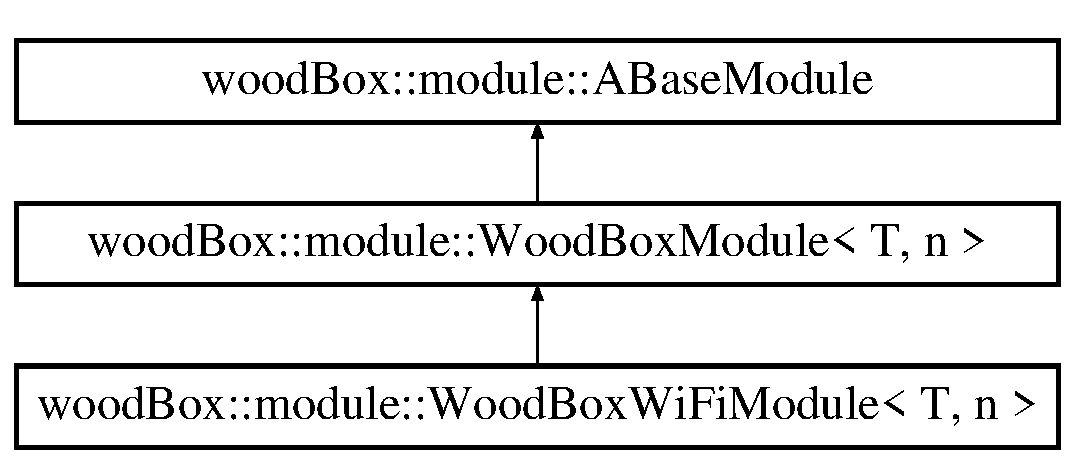
\includegraphics[height=3.000000cm]{classwood_box_1_1module_1_1_wood_box_wi_fi_module}
\end{center}
\end{figure}
\subsection*{Public Member Functions}
\begin{DoxyCompactItemize}
\item 
\mbox{\Hypertarget{classwood_box_1_1module_1_1_wood_box_wi_fi_module_aac99d548520fa9c5f5a29aa99bdc241d}\label{classwood_box_1_1module_1_1_wood_box_wi_fi_module_aac99d548520fa9c5f5a29aa99bdc241d}} 
{\bfseries Wood\+Box\+Wi\+Fi\+Module} (const \mbox{\hyperlink{classwood_box_1_1module_1_1_wood_box_wi_fi_module}{Wood\+Box\+Wi\+Fi\+Module}} \&)=delete
\item 
\mbox{\Hypertarget{classwood_box_1_1module_1_1_wood_box_wi_fi_module_aba3f7e5c892542d70db28130eddb3084}\label{classwood_box_1_1module_1_1_wood_box_wi_fi_module_aba3f7e5c892542d70db28130eddb3084}} 
\mbox{\hyperlink{classwood_box_1_1module_1_1_wood_box_wi_fi_module}{Wood\+Box\+Wi\+Fi\+Module}} \& {\bfseries operator=} (const \mbox{\hyperlink{classwood_box_1_1module_1_1_wood_box_wi_fi_module}{Wood\+Box\+Wi\+Fi\+Module}} \&)=delete
\item 
\mbox{\Hypertarget{classwood_box_1_1module_1_1_wood_box_wi_fi_module_ad1fa85749c0e194c9e589261dfb2433d}\label{classwood_box_1_1module_1_1_wood_box_wi_fi_module_ad1fa85749c0e194c9e589261dfb2433d}} 
void {\bfseries set\+Wi\+Fi\+Communicator} (\mbox{\hyperlink{classwood_box_1_1communication_1_1wifi_1_1_a_wi_fi_communicator}{communication\+::wifi\+::\+A\+Wi\+Fi\+Communicator}} \&wifi)
\end{DoxyCompactItemize}
\subsection*{Friends}
\begin{DoxyCompactItemize}
\item 
\mbox{\Hypertarget{classwood_box_1_1module_1_1_wood_box_wi_fi_module_a63a1b80c5bfd6525d93f1b3dc9dab20b}\label{classwood_box_1_1module_1_1_wood_box_wi_fi_module_a63a1b80c5bfd6525d93f1b3dc9dab20b}} 
class {\bfseries Wood\+Box\+Module$<$ T, n $>$}
\end{DoxyCompactItemize}
\subsection*{Additional Inherited Members}


The documentation for this class was generated from the following file\+:\begin{DoxyCompactItemize}
\item 
Wood\+Box\+Wi\+Fi\+Module.\+hpp\end{DoxyCompactItemize}

%--- End generated contents ---

% Index
\backmatter
\newpage
\phantomsection
\clearemptydoublepage
\addcontentsline{toc}{chapter}{Index}
\printindex

\end{document}
